\chapter{Hadronic recoil calibration}\label{sec:HadrCalib}
\minitoc

\etmiss affects significantly the W boson measurement, so it is important to have a solid understanding  of possible of sources differences in the hadron recoil reconstruction in data and Monte Carlo. This chapter describes the procedure of calibration bias and resolution mismodelling in a hadron recoil, that was adapted for 2.76 TeV data. 

\section{Introduction}
\begin{figure}[!bp]
\centering
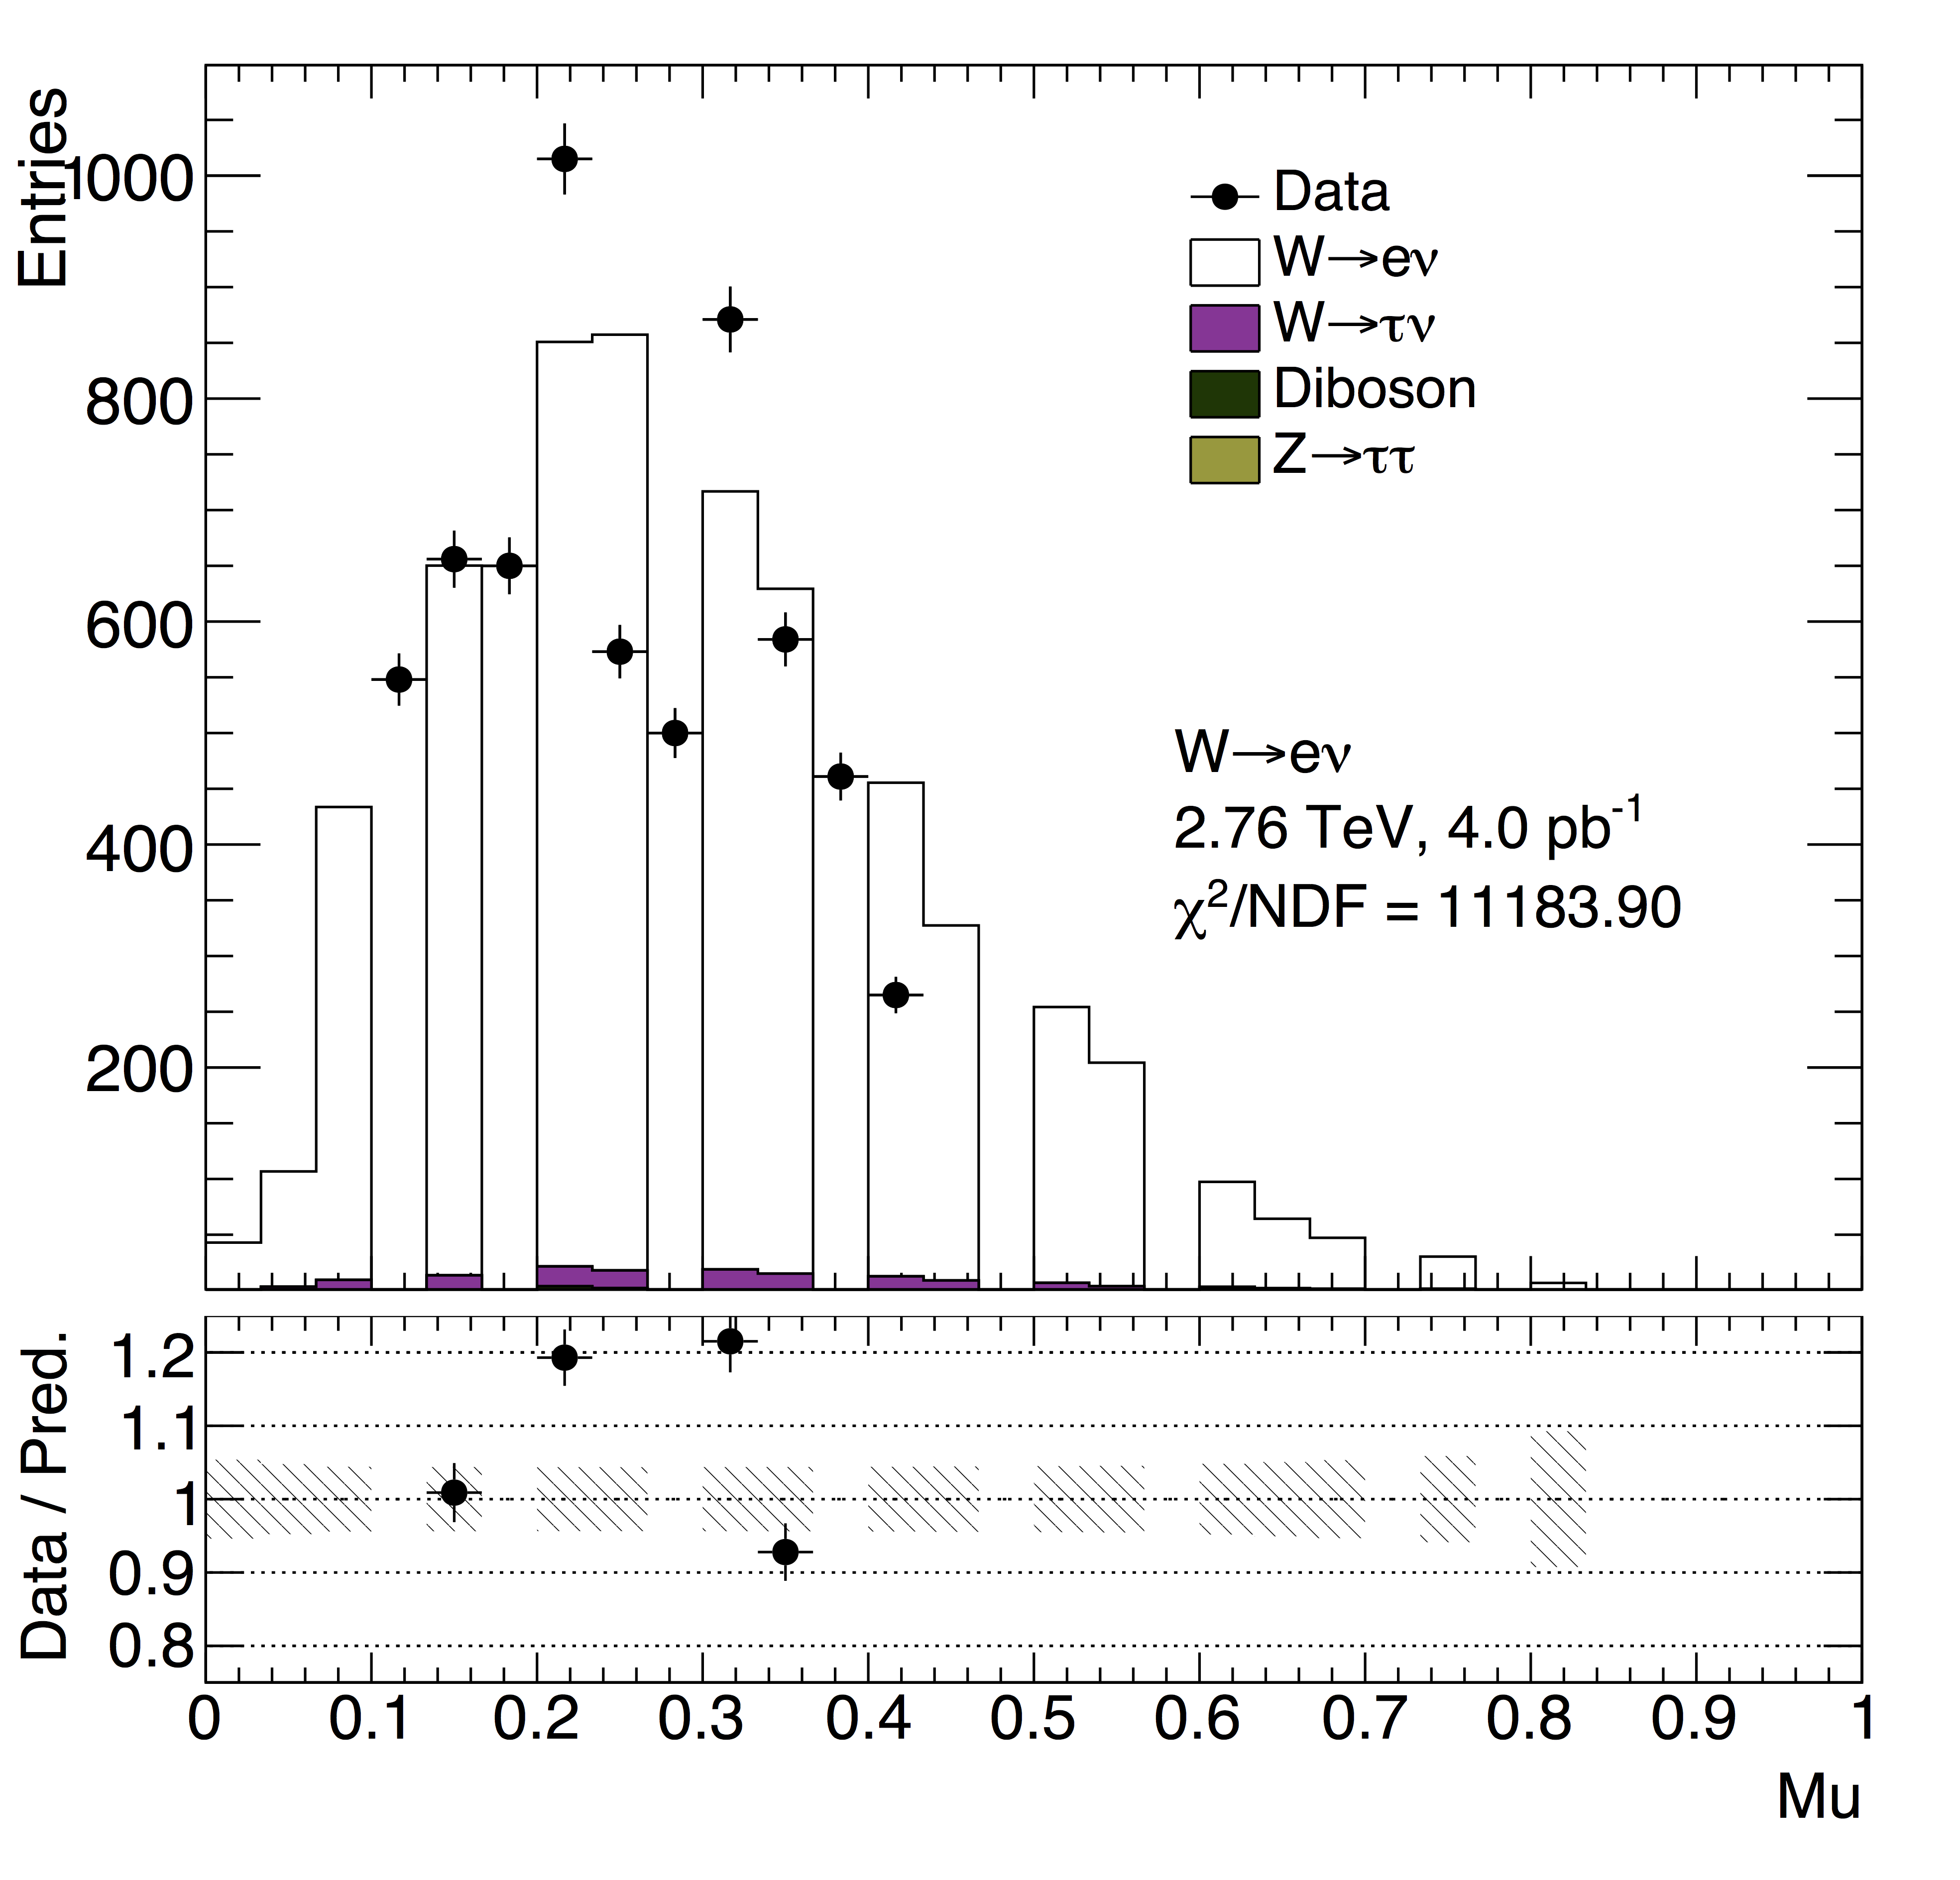
\includegraphics[width=0.5\textwidth]{HadronRecoil/W_Event_Mu.png}
\caption{Mean number of interactions per bunch crossing from the \wenu selection. MC modelled pileup discretelly, that makes a standard data to MC reweighting procedure not feasible.}
\label{HadrRecoil:mu}
\end{figure} 

\begin{figure}[!tbp]
\begin{center}
\begin{minipage}[h]{0.49\linewidth}
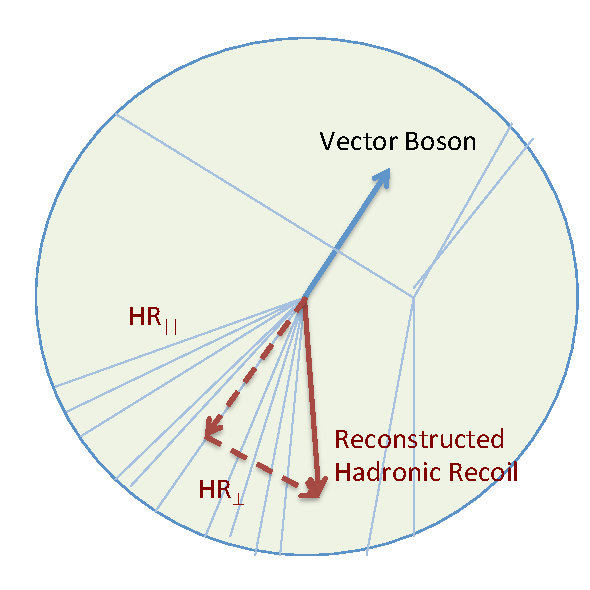
\includegraphics[width=1\textwidth]{HadronRecoil/RecoHRParPerp.pdf}
\end{minipage}
\caption{Parallel and perpendicular projections of the hadronic recoil with respect to the transverse momentum of the vector boson \cite{HRPlots}}
\label{ris:HadrRecoilTruthPt}
\end{center}
\end{figure}

This analysis uses a standard hadronic recoil calibration procedure, described in \cite{HRCorrections}, that was modified and adapted for the low statistics 2.76 TeV case. The standart procedure consist of the 3 main steps. 

The first step in a hadronic recoil calibration procedure aim to correct differences in a pile-up modeling in the event. Additional interactions can have a significant effect on a \etmiss and \sumet distributions. This discrepancies are usually corrected by reweighting average number of interactions per bunch crossing in MC to match the data. However, \atlas simulation is suited for high pile-up runs, so this quantity is modelled discretly in case of 2.76 TeV analysis (Fig. \ref{HadrRecoil:mu}), what makes the precises reweighting impossible. However, since the mean number is below 1, effect of these discrepancies on \etmiss distributions can be neglected. 

On the second and third step possible discrepancies in a resolution and scale of hadroninc recoil respectively are corrected. The hadronic recoil algorithm performance can be studied in MC through the projection of $\vec{HR}$ on the direction of the transverse momentum of the vector boson, as shown in Fig. \ref{ris:HadrRecoilTruthPt}. This projection can be divided into perpendicular \uperp and parallel \upar component as follows:
\begin{equation}
\upar=\vec{v_{xy}}\cdot\vec{HR}
\end{equation}
\begin{equation}
\uperp=v_x\cdot HR_y - v_y \cdot HR_x,
\end{equation}
where $\vec{v_{xy}}$ is a unitary vector along the transverse component of a vector boson momentum and $v_x$ and $v_y$ are its projections on x and y axis respectively. In the case of the true kinematics $\upar=p_T^{bos}$ and $\uperp = 0$. However the calorimeter resolution is causing relatively wide distributions for these projections. The parallel component \upar is sensitive to a possible bias in the hadron recoil, while the perpendicular \uperp can be used for determination of the resolution discrepancies. The mean and the width of these distributions can depend on different variables, such as a mean number of interactions in event, hadronic activity, boson $P_{T}^{bos}$ etc. 

It is convinient to use Z boson decays for a hadron recoil calibration, since its transverse momentum $P_T^Z$ can be determined not only from the hadronic recoil, but also from its decay products.  The $P_T^Z$ resolution coming from a lepton reconstruction is 3-4 times more precise, than the one extracted from a hadronic recoil. This allows to treat leptonically reconstructed $P_T^{Z}$ as a reference $P_T$ of the boson and to compare directly \uperp and \upar in data and MC. However, small size of the Z sample in 2.76TeV data leads to a high statistics error for these distributions. The calibration constants can also be  derived from W boson decays. In order to exclude possible bias from $P_T^W$ mismodelling these calibration constants can be derived through data vs MC comparison of $P_T^{W}$ independent distributions (such as \mtw). The combined Z and W boson determination procedure has been used. 

\section{Hadronic recoil resolution correction}

\begin{figure}[!tbp]
\begin{center}

\begin{minipage}[h]{0.7\linewidth}
\center{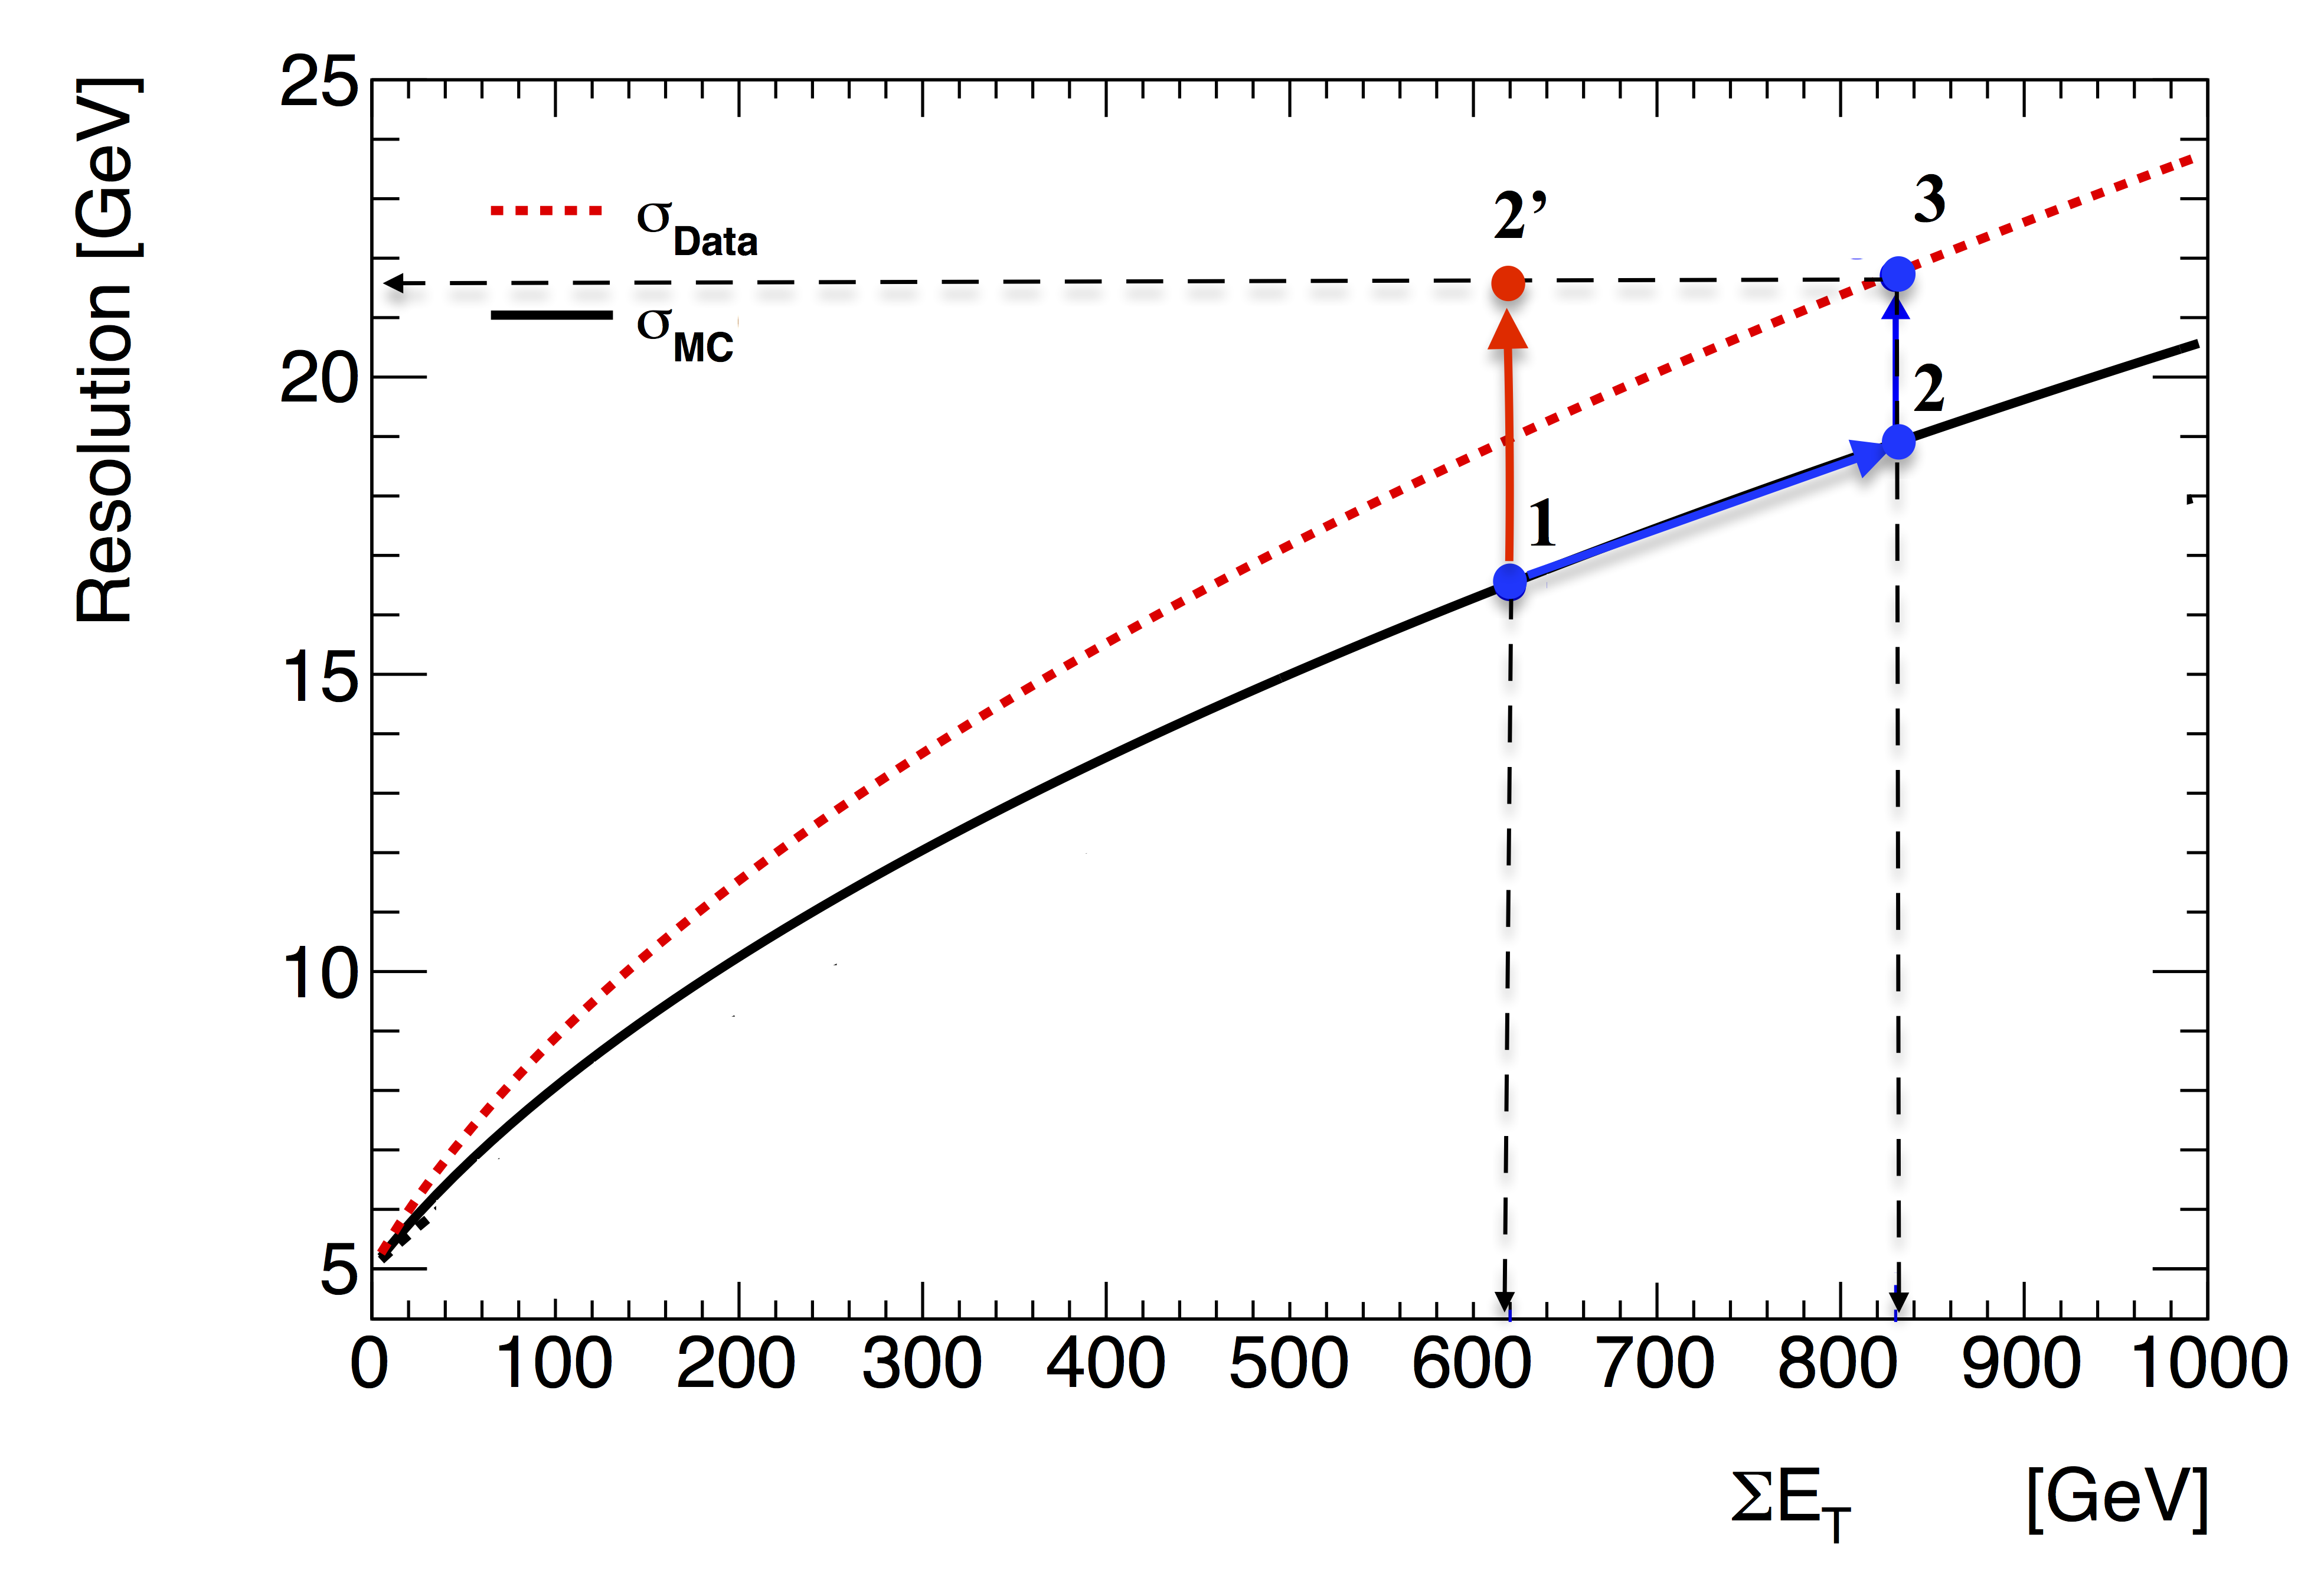
\includegraphics[width=1.\linewidth]{HadronRecoil/sumet.png}}
\end{minipage}

\end{center}
\caption{Schematic view of the correction procedure: this figure illustrates the resolution of \uperp as a function of \sumet. The dotted curve represents data resolution ($\sigma_{data}$), solid black is a nominal MC ($\sigma_{MC}$). Blue line from point 1 to point 2 corresponds to a \sumet correction discussed in Sec.\ref{sec:SumetCor}. Red line from point 1 to point 2' corresponds to a direct correction of resolution mismodelling discussed in Sec. \ref{sec:ZperpSmear}. Modified from \cite{HRCorrections}}

\label{ris:sumetCor}
\end{figure}


The event activity plays an important role in the \etmiss reconstruction. Since \sumet and the hadronic recoil resolution values are correlated, the possible mismodelling of the event activity can lead to differences between the data and Monte Carlo \etmiss resolutions (Fig. \ref{ris:sumetCor}). There are two ways of resolution correction in the 2.76 TeV data:
\begin{itemize}
\item As a two step procedure, shown as path 1-2-3 in Fig. \ref{ris:sumetCor}. The first step is to correct sumet distribution to match the data using reweighting of the events. Remaining differences in resolution are corrected at the second step. This method is discussed Sec. \ref{sec:SumetCor}. 
\item The second order effects on \etmiss coming from \sumet modelling are neglected and the resolution differences between data and MC corrected directly. This procedure matched to the path 1-2' in Fig. \ref{ris:sumetCor} and described in Sec. \ref{sec:ZperpSmear}.
\end{itemize}


\subsection{\sumet distribution correction}\label{sec:SumetCor}



\begin{figure}[!tbp]
\begin{minipage}[h]{0.5\linewidth}
\center{\includegraphics[width=1.\linewidth]{HadronRecoil/UncorrSumet/W_EtMiss_CorRecoilSumet.pdf} \\ a)}
\end{minipage}
\hfill
\begin{minipage}[h]{0.5\linewidth}
\center{\includegraphics[width=1.\linewidth]{HadronRecoil/UncorrSumet/Wmu_EtMiss_CorRecoilSumet.pdf} \\ b)}
\end{minipage}
\caption{Event activity \sumet distribution from a) the \wenu selection and b) the \wmunu selection. There is a clear sign of the event activity mismodelling in both channels, that should be corrected.}
\label{HadrRecoil:UncorrSumet}
\end{figure}

\begin{figure}[!tbp]
\begin{minipage}[h]{0.5\linewidth}
\center{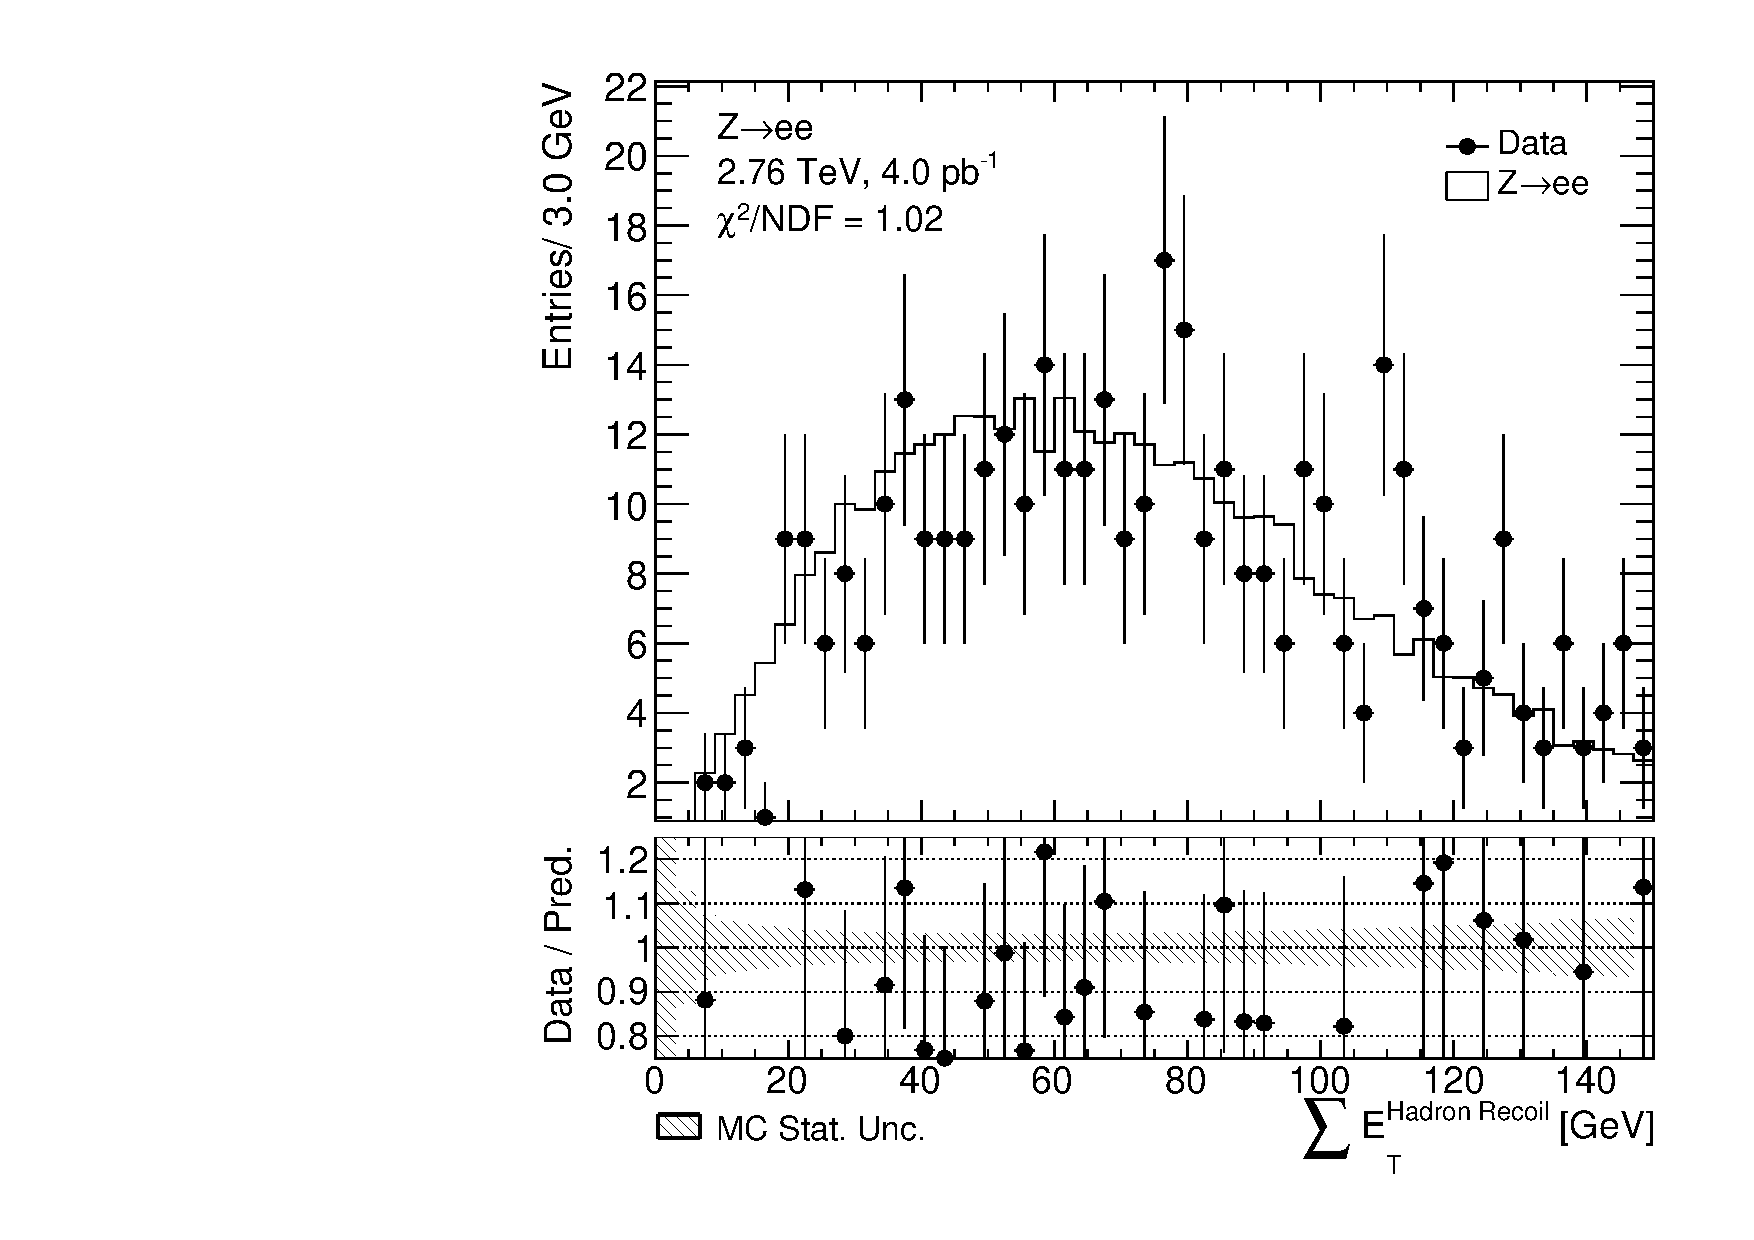
\includegraphics[width=1.\linewidth]{HadronRecoil/ZeeSumet.pdf} \\ a)}
\end{minipage}
\hfill
\begin{minipage}[h]{0.5\linewidth}
\center{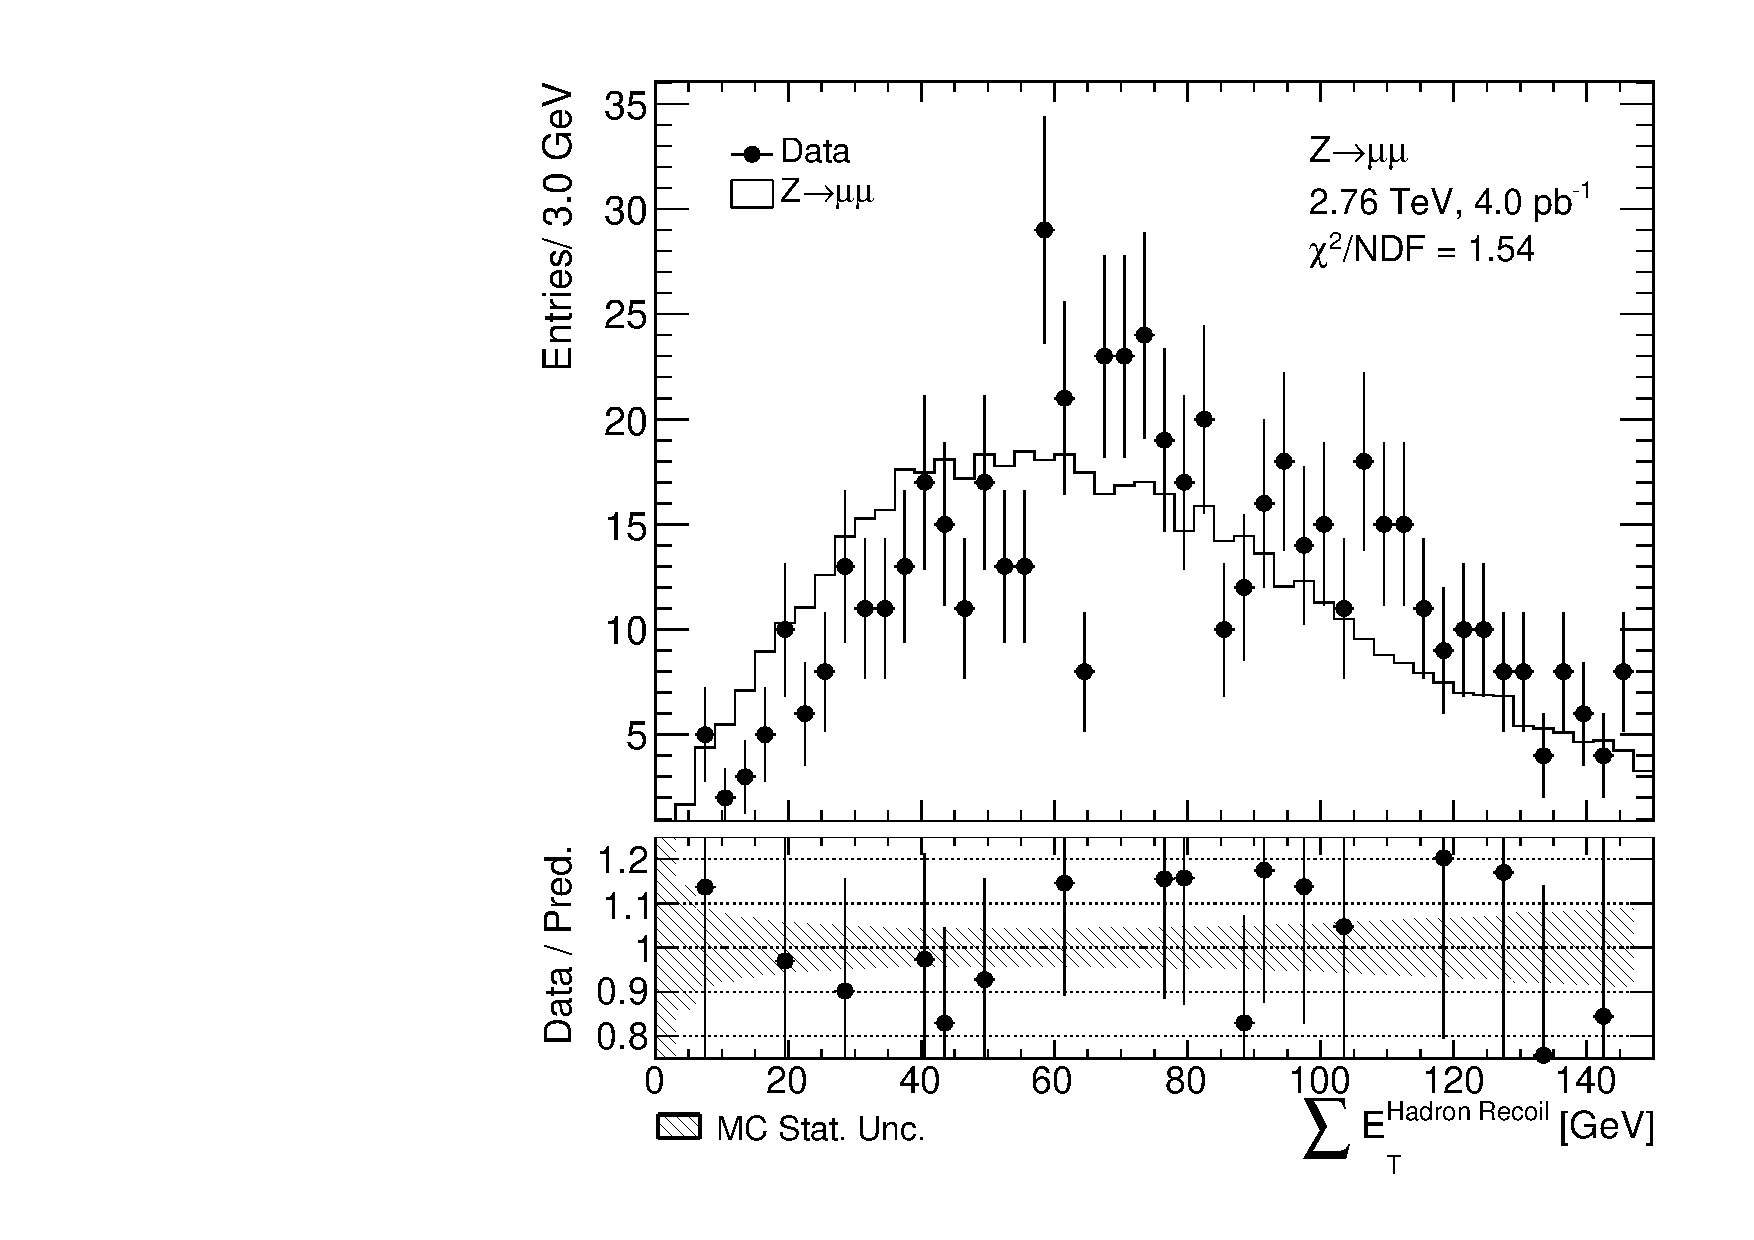
\includegraphics[width=1.\linewidth]{HadronRecoil/ZmumuSumet.pdf} \\ b)}
\end{minipage}
\caption{Event activity \sumet distribution from a) the $Z\to ee$ selection and b) the $Z\to \mu\mu$ selection. Size of the Z sample in 2.76 TeV data is insufficient indicate to the mismodelling of the event activity. }
\label{HadronRecoilSumetZ}
\end{figure}

\begin{figure}[!tbp]
\center{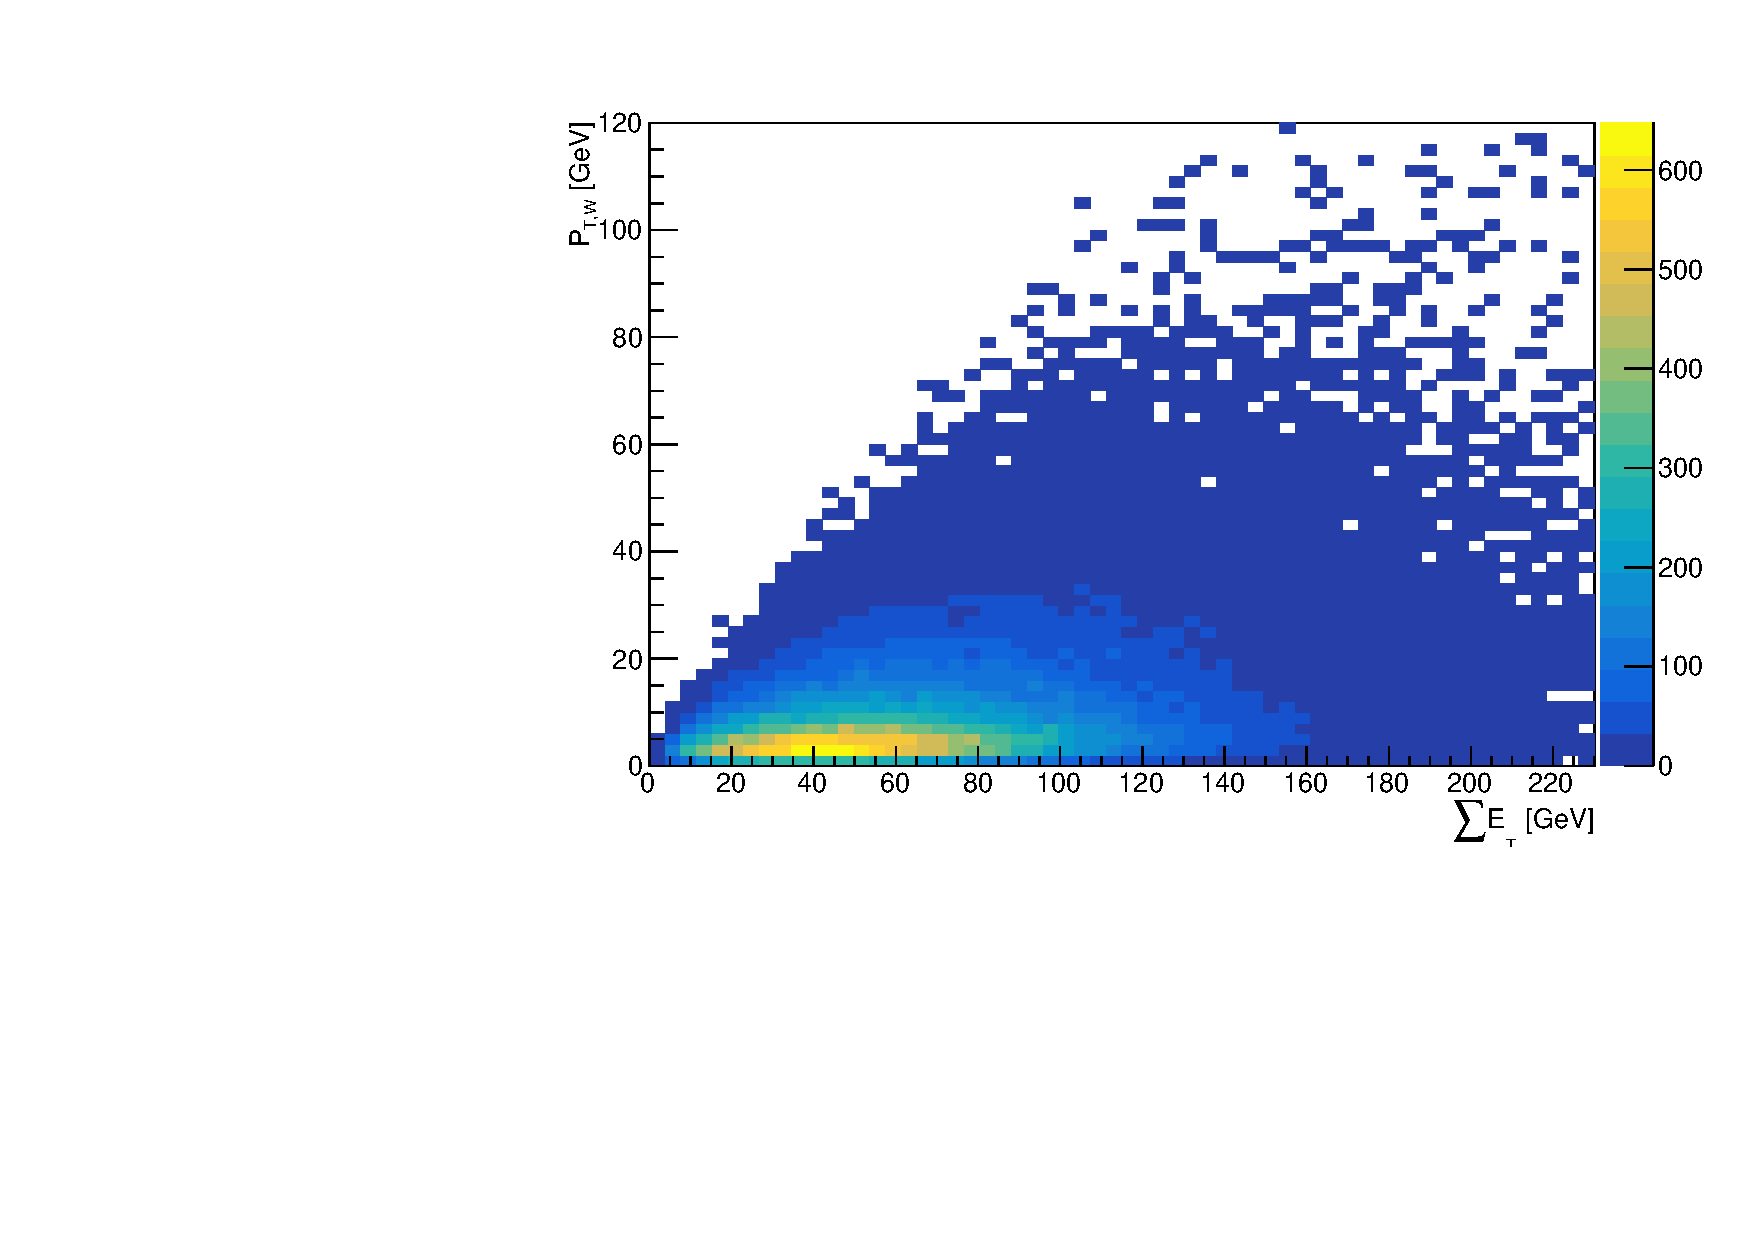
\includegraphics[width=1.\linewidth]{HadronRecoil/SumetPtTruth.pdf} }
\caption{Distribution of event activity \sumet vs truth transverse momentum of the W boson \ptw$^{truth}$ in the $W^{+} \to e\nu$ MC sample.  }
\label{HadrRecoil:SumetPt}
\end{figure}




The distributions of the event activity \sumet  are shown in a Fig. \ref{HadrRecoil:UncorrSumet}. There is a visible shift between data and MC distribution for both W boson channels. Standard procedure, used in \mtw measurment at 7 TeV uses a smirnov transformation of \sumet distributions in Z events. Unfortunatelly, size of the Z sample is not sufficient for this procedure (Fig. ~\ref{HadronRecoilSumetZ}). This motivates a choise of \sumet reweighting constants determination from the W boson sample. 

The event activity \sumet is correlated to the truth transverse momentum of the boson, as shown in Fig. \ref{HadrRecoil:SumetPt}, so in order to avoid possible bias from changing \ptw spectrum, reweighting constants are derived in bins of reconstructed boson momentum $P_T^{W, rec}$. Inside each $P_T^{W, rec}$ bin reweighting constants are calculated as:
\begin{equation}
SF^{channel}=\frac{\sum E_T^{data, \, selection} }{\sum E_T^{MC,\, no\, cuts} },
\end{equation}
where $\sum E_T^{data,\, selection} $ is a \sumet distribution inside a given $P_T^{W, rec}$ after the full event selection. In order to reduce systematic error from this value, a combination of \wenu and \wmunu events is used.  Second term $\sum E_T^{MC,\, no\, cuts}$ is  \sumet distribution in MC before any selection. Scale factors are determined separately for each signal MC for W boson decays, in order to leave the total number of events in MC after correction untouched. Transverse boson momentum binning is choosen so what there is an approximate equality in total number of events between bins. The total number of $P_T^{W, rec}$ bins is 6.
Example of correction factors for two different $P_T^{W, rec}$ bins are shown on a Fig.\ref{ris:SumEtCorPtW}. Resulting reweighting constants for \wenu and \wmunu MC samples are shown in Fig. \ref{ris:SumEtCorNoPol}. This method allows to leave the reconstructed transverse momentum of the boson untouched and introduces a small change in a truth boson spectrum, as shown on Fig. \ref{HadrRecoil:PtSpectrum}.

\begin{figure}[!tbp]
\begin{minipage}[h]{0.49\linewidth}
\center{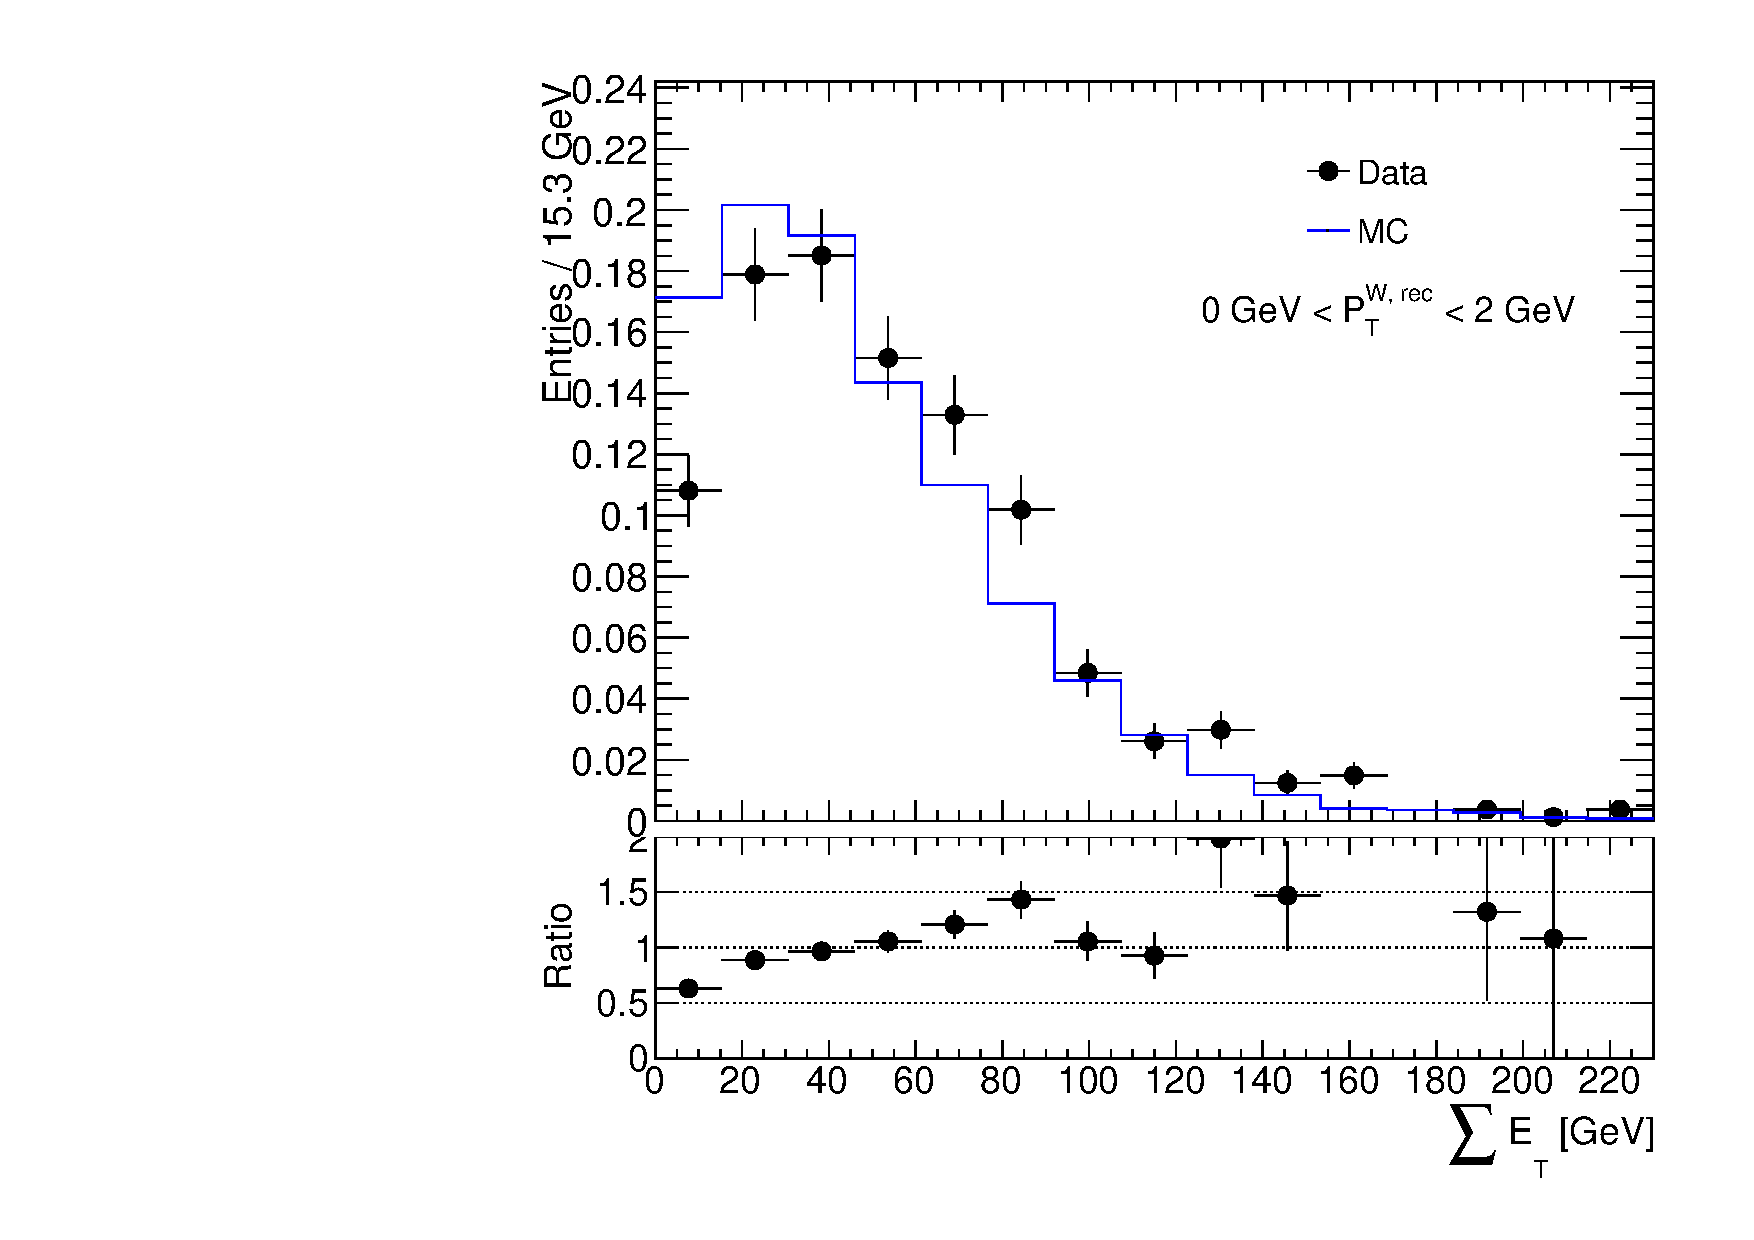
\includegraphics[width=1.\linewidth]{HadronRecoil/2.pdf} \\ a)}
\end{minipage}
\hfill
\begin{minipage}[h]{0.49\linewidth}
\center{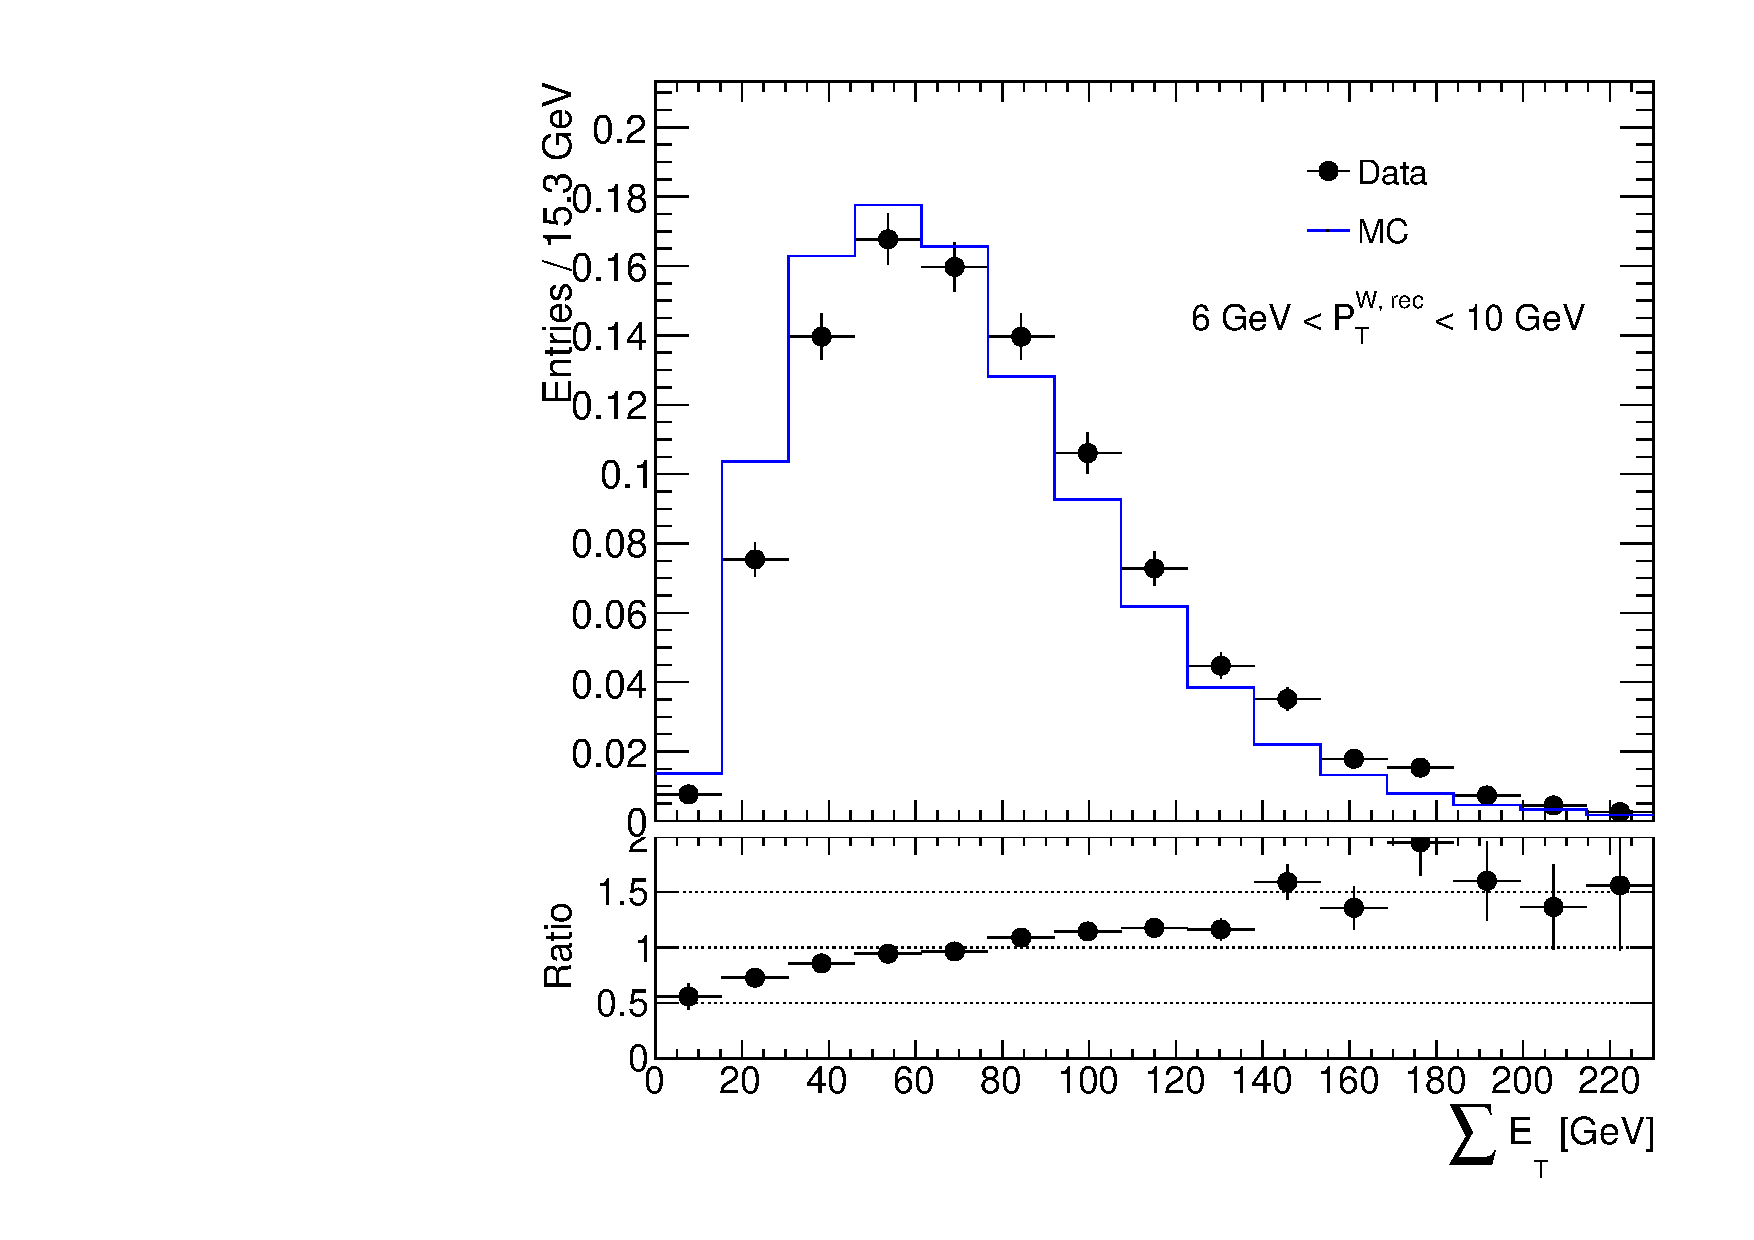
\includegraphics[width=1.\linewidth]{HadronRecoil/10.pdf} \\ b)}
\end{minipage}
\caption{Distribution of \sumet for the different $p_T^{W, rec}$ bins for $W^{+} \to e \nu$ MC sample}
\label{ris:SumEtCorPtW}
\end{figure}

\begin{figure}[!tbp]
\begin{minipage}[h]{0.49\linewidth}
\center{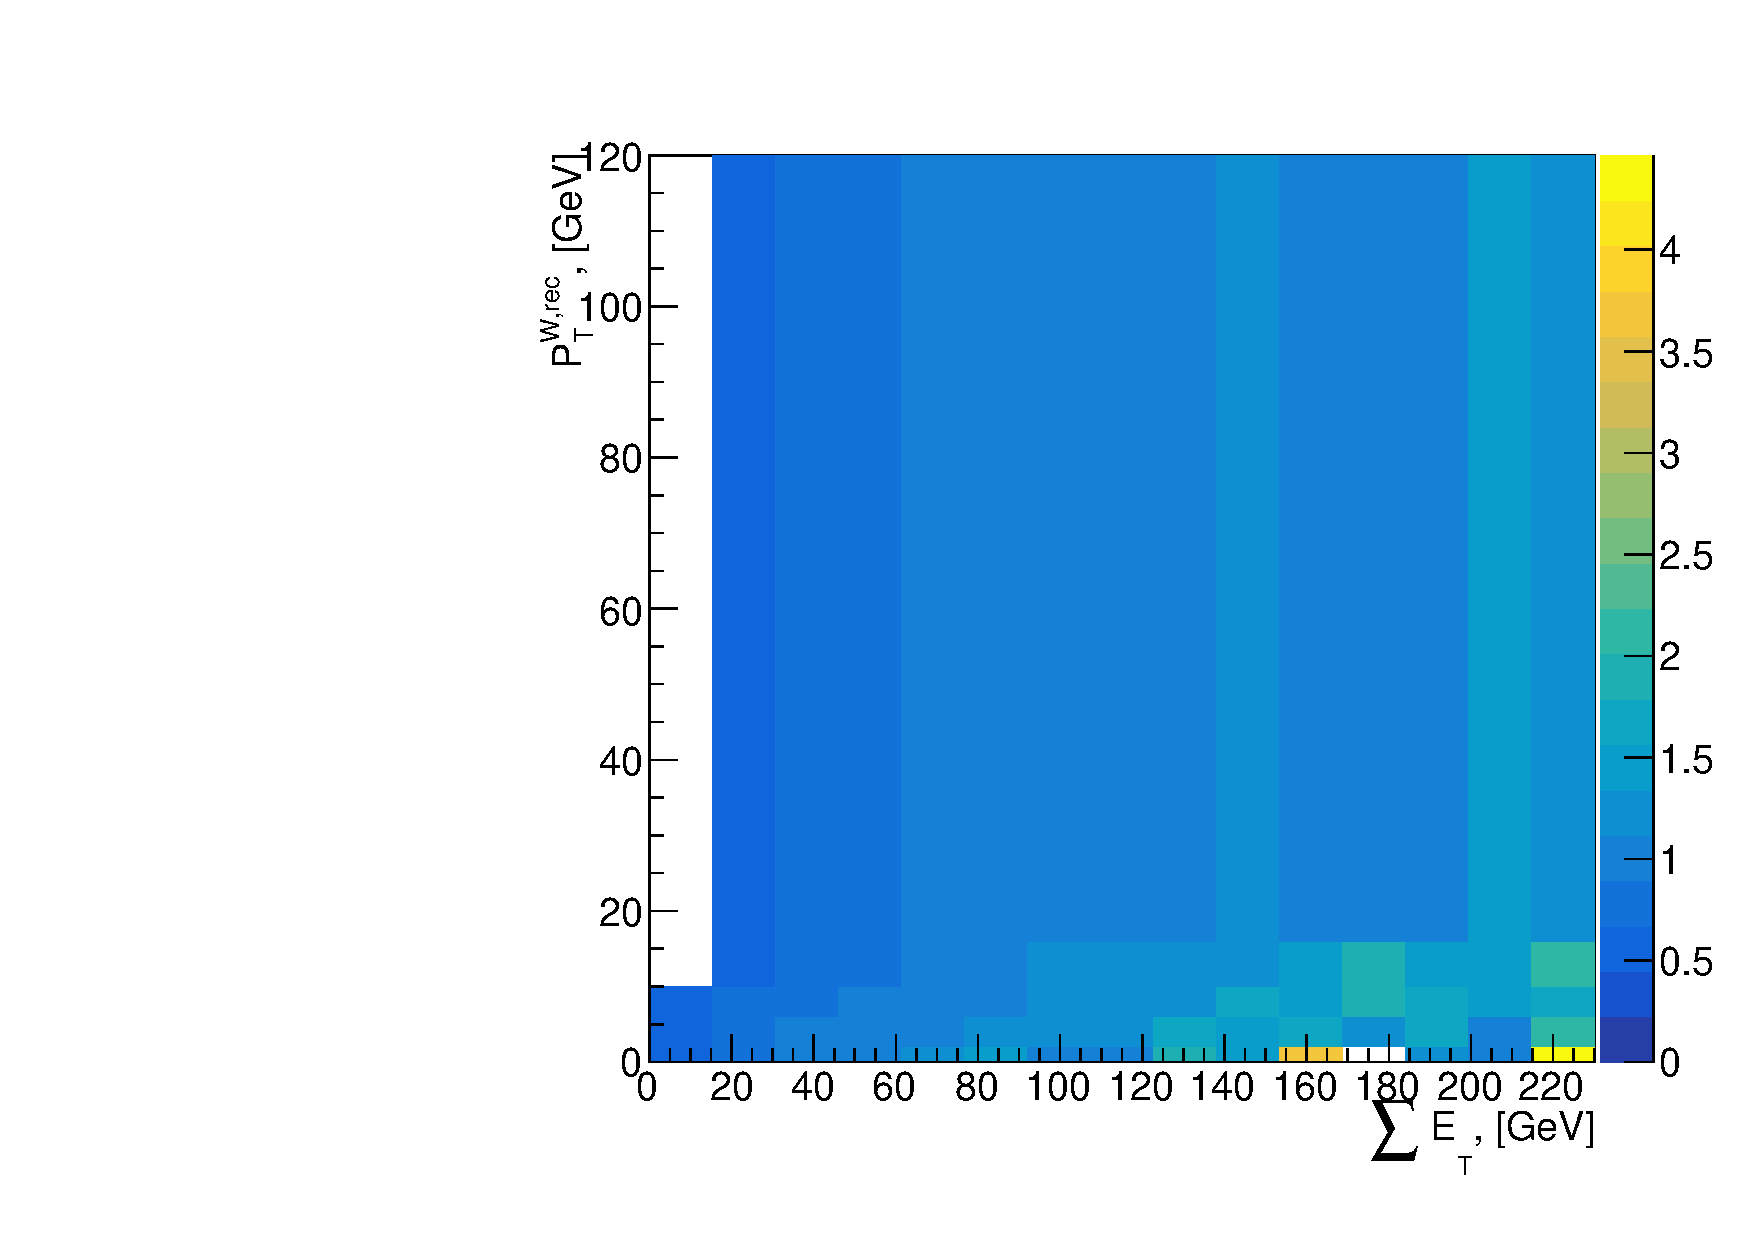
\includegraphics[width=1.\linewidth]{HadronRecoil/ReweightingNoPolEP.pdf} \\ a)}
\end{minipage}
\hfill
\begin{minipage}[h]{0.49\linewidth}
\center{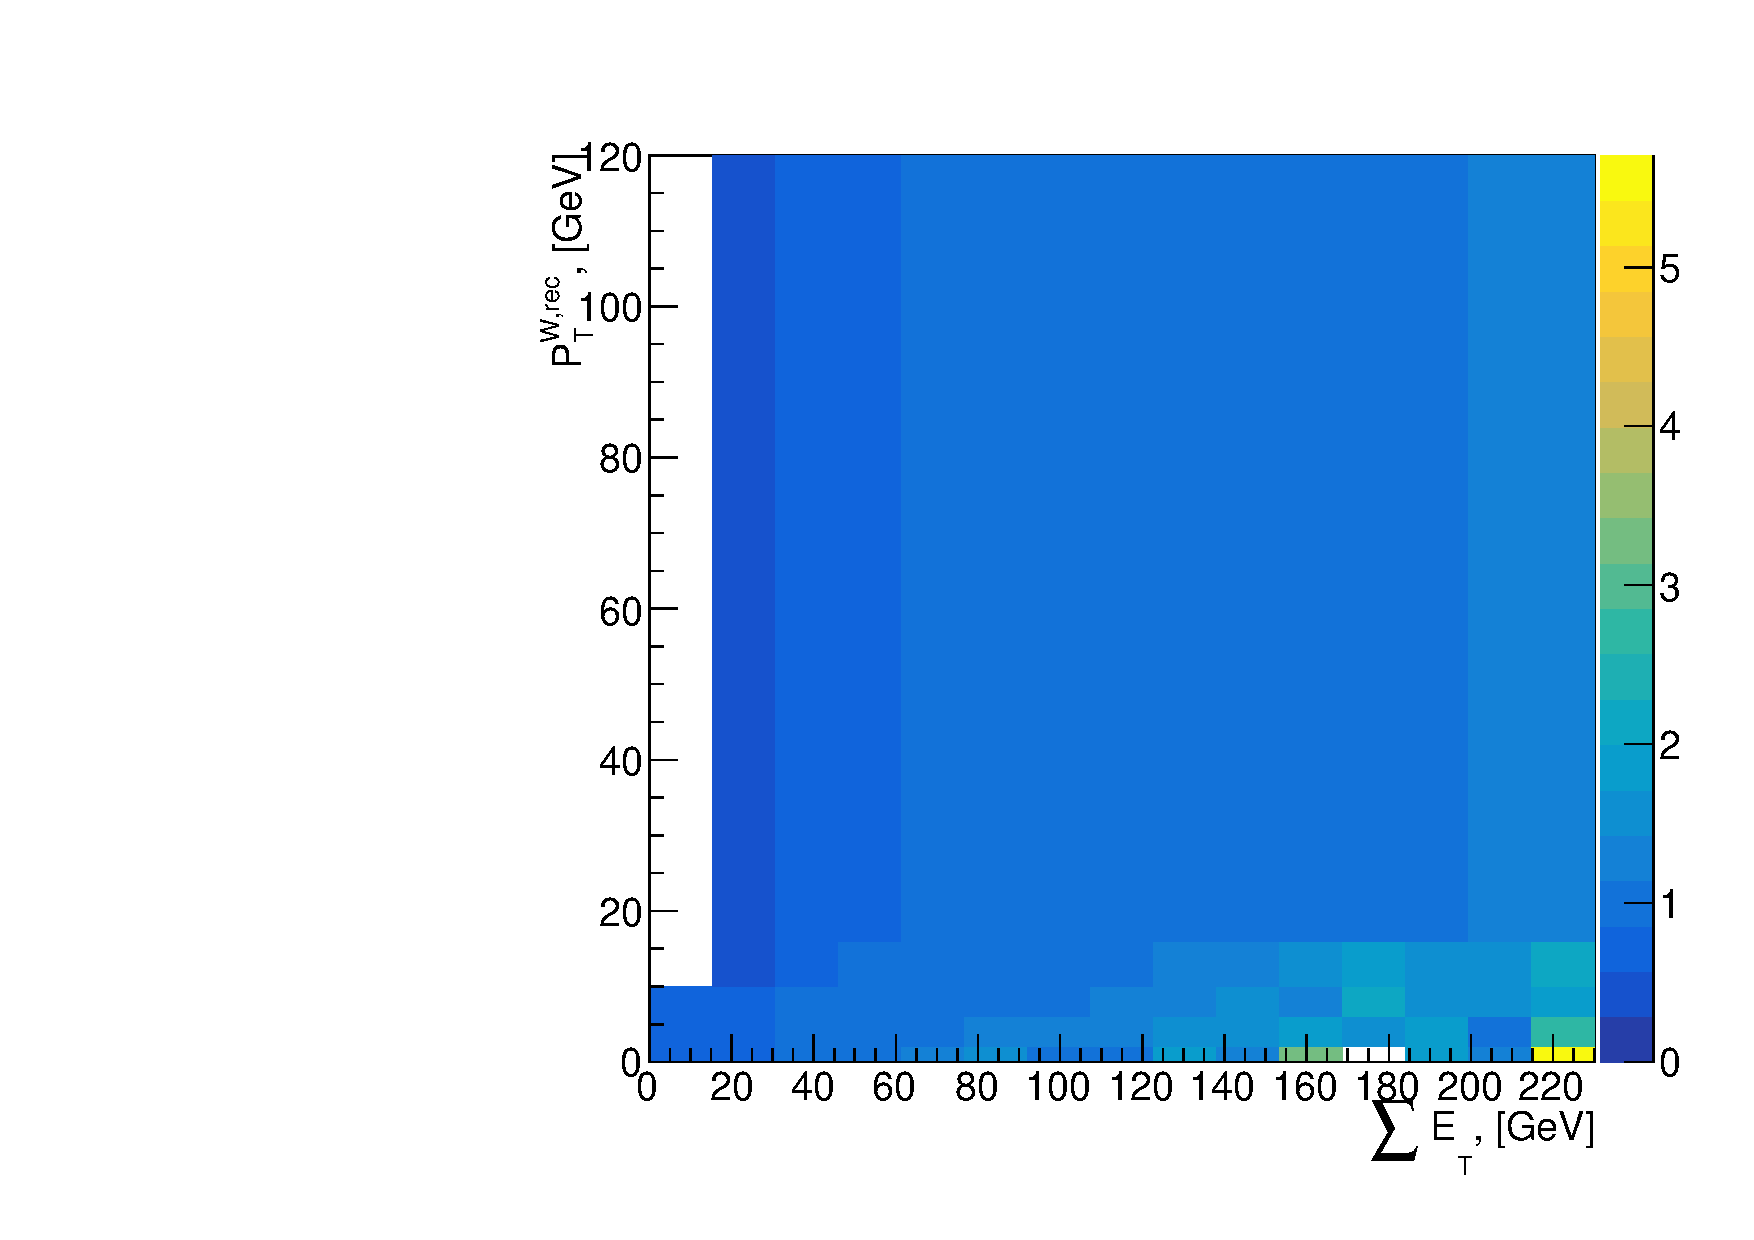
\includegraphics[width=1.\linewidth]{HadronRecoil/ReweightingNoPolMP.pdf} \\ b)}
\end{minipage}
\caption{Distribution of \sumet reweighting constants derived for a) $W^{+} \to e \nu$ and b) $W^{+} \to \mu \nu$ MC sample.}
\label{ris:SumEtCorNoPol}
\end{figure}

\begin{figure}[!tbp]
\begin{minipage}[h]{0.5\linewidth}
\center{\includegraphics[width=1.\linewidth]{HadronRecoil/CorrSumet/W_EtMiss_CorRecoilSumet.pdf} \\ a)}
\end{minipage}
\hfill
\begin{minipage}[h]{0.5\linewidth}
\center{\includegraphics[width=1.\linewidth]{HadronRecoil/CorrSumet/Wmu_EtMiss_CorRecoilSumet.pdf} \\ b)}
\end{minipage}
\caption{Event activity \sumet distribution from a) the \wenu selection and b) the \wmunu selection after \sumet correction. }
\label{HadrRecoil:CorrSumet}
\end{figure}

\begin{figure}[!tbp]
\begin{minipage}[h]{0.49\linewidth}
\center{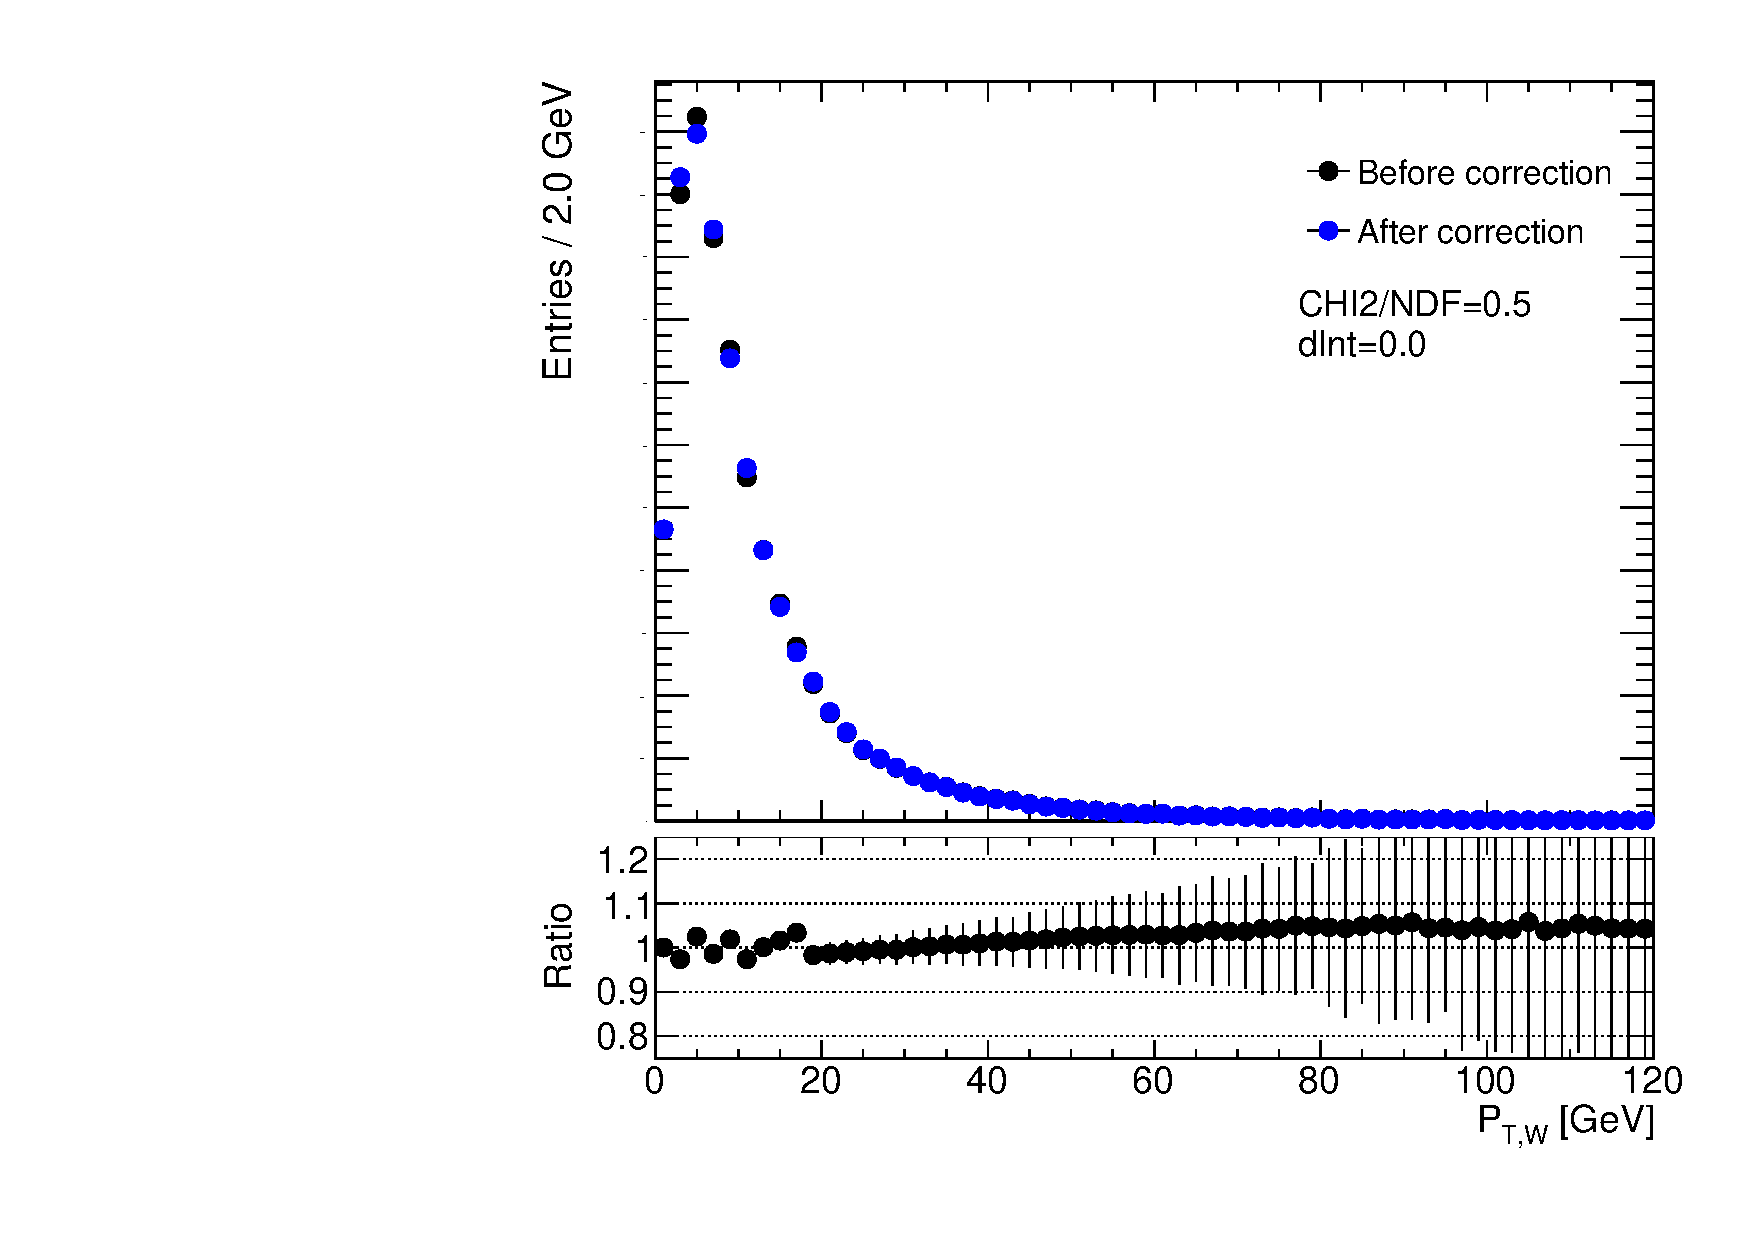
\includegraphics[width=1.\linewidth]{HadronRecoil/WplusenuRecoEffect.pdf} \\ a)}
\end{minipage}
\hfill
\begin{minipage}[h]{0.49\linewidth}
\center{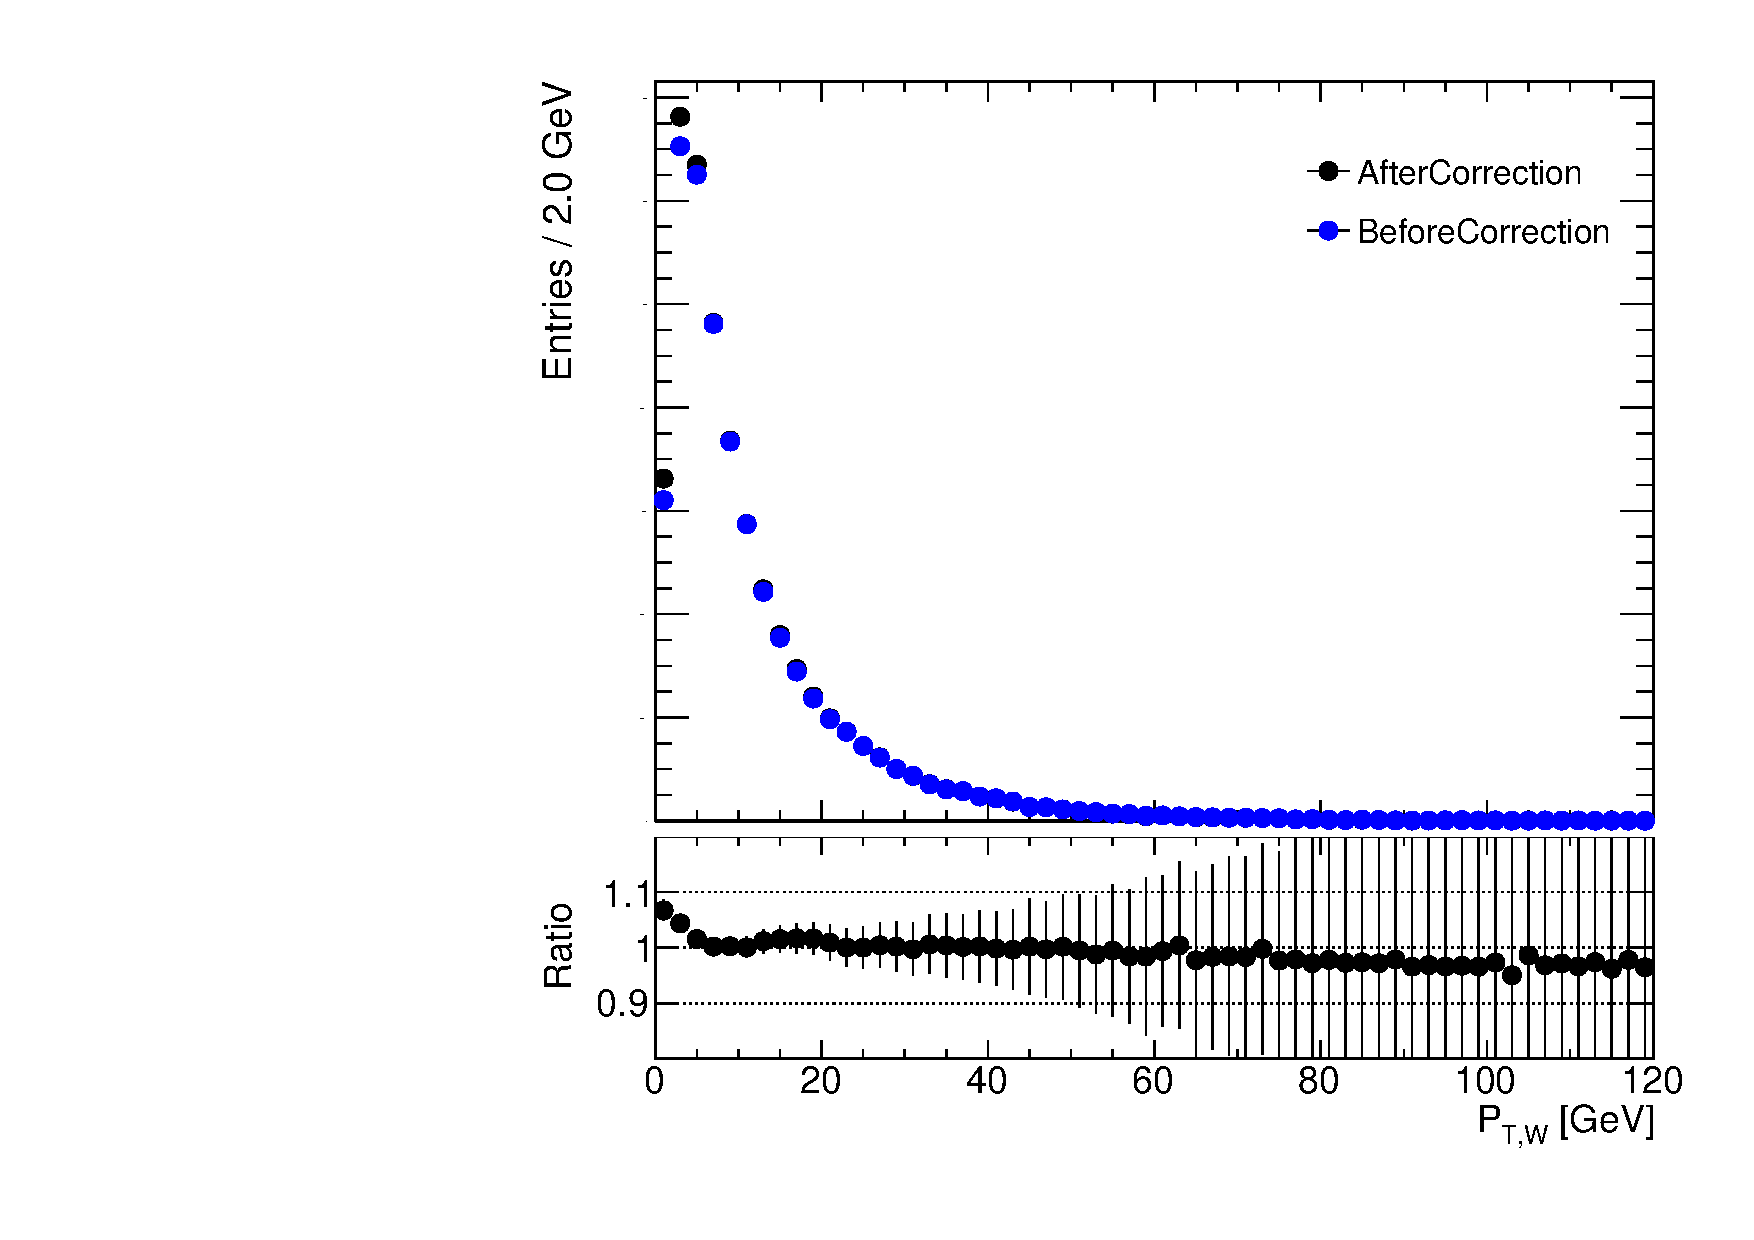
\includegraphics[width=1.\linewidth]{HadronRecoil/Wplusenu.pdf} \\ b)}
\end{minipage}
\caption{Effect of the \sumet reweighting on a) reconstructed transverse momentum of the boson and b) truth transverse momentum of the boson in $W^{+} \to e\nu$ MC sample.}
\label{HadrRecoil:PtSpectrum}
\end{figure}

\subsubsection{Systematic error estimation}

Systematic error on this reweighting can be estimated using the approximation of the ration inside each $P_T^{W, rec}$ bin by a polynomial degree 2 or 1. This method also allows to neglect effect of the data fluctuations, especially for high \sumet regions, that could be seen on a Fig. \ref{ris:SumEtCorNoPol}. Because of the low statistics for \sumet > 220 GeV ratio in the last bins have been set to 1 and this region haven't been included in the polynomial fit. Total reweigting constants obtained from this procedure are shown on a Fig. \ref{ris:SumEtCorPol}. 

\begin{figure}[!tbp]
\begin{minipage}[h]{0.49\linewidth}
\center{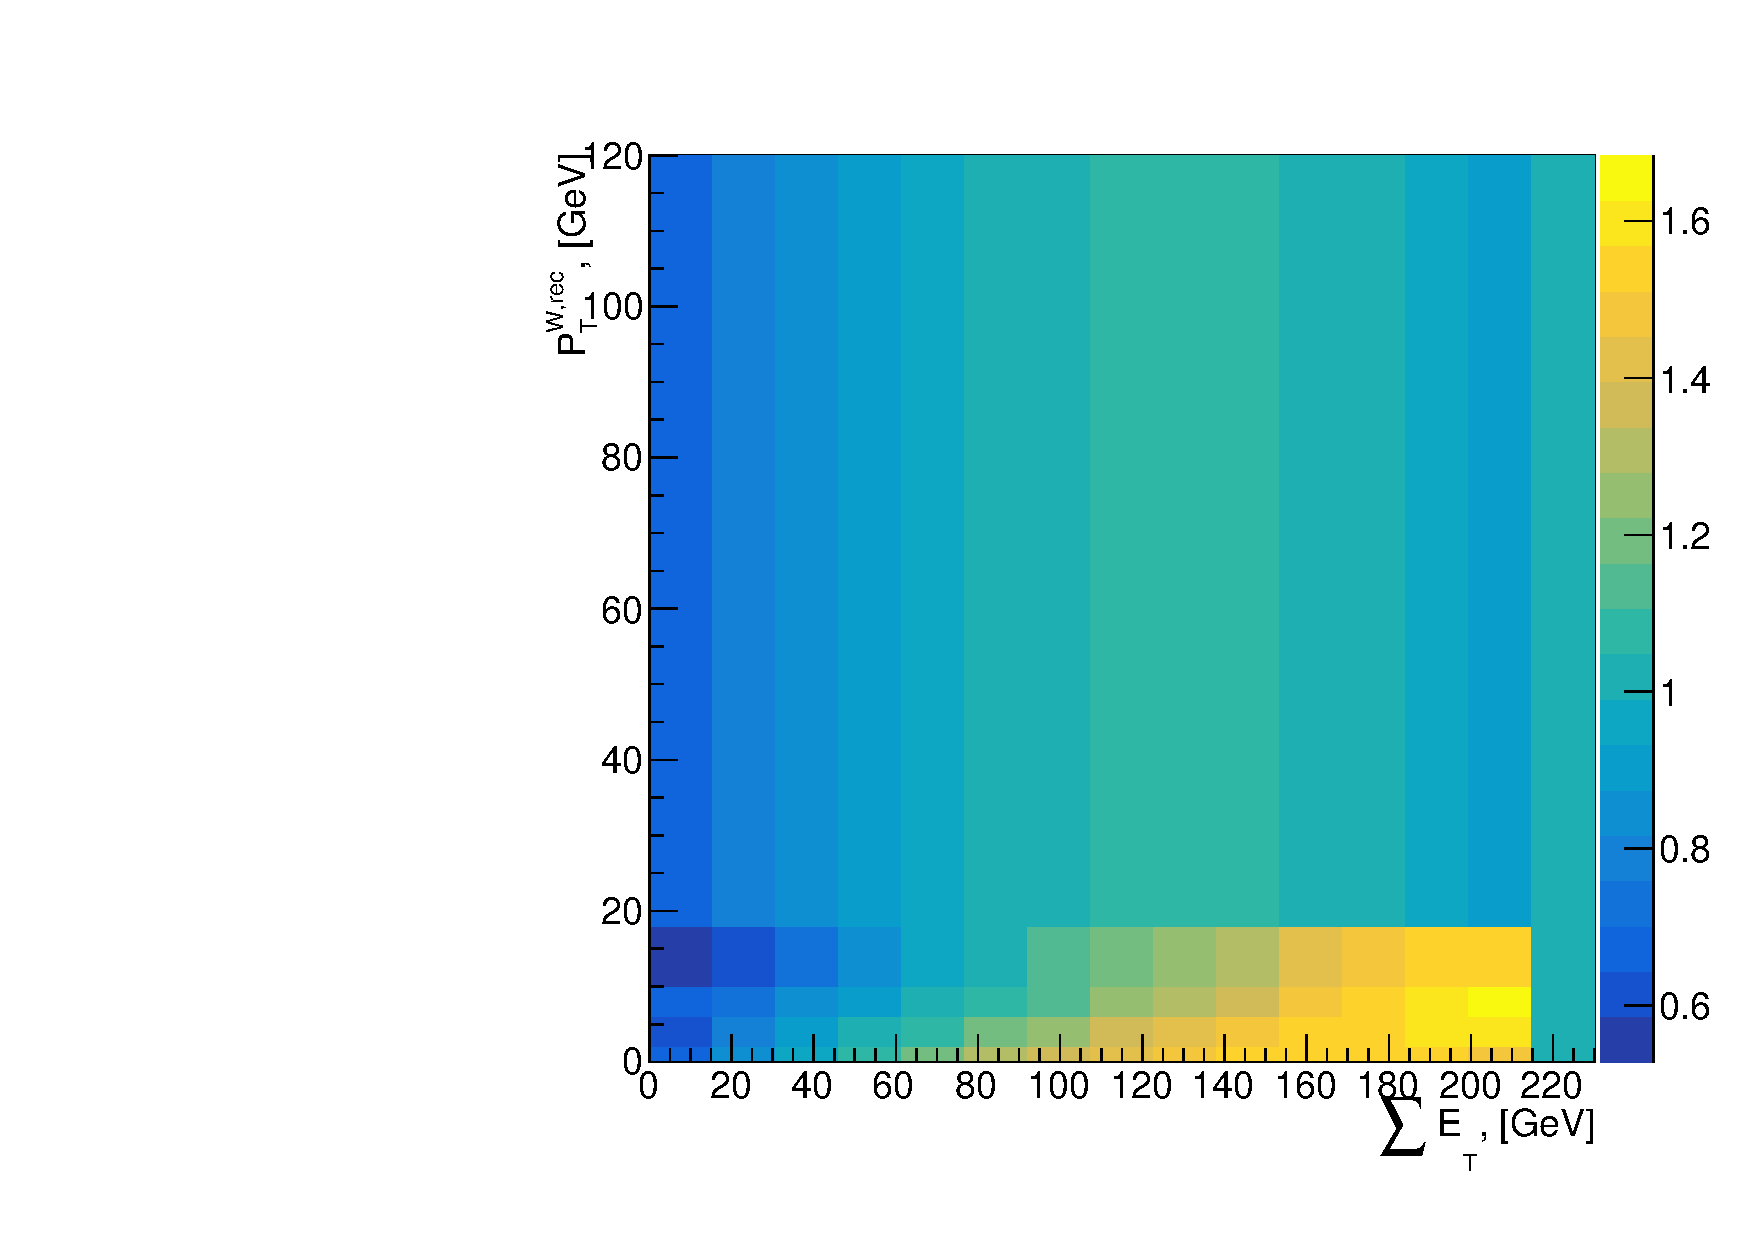
\includegraphics[width=1.\linewidth]{HadronRecoil/ReweightingPolEP.pdf} \\ a)}
\end{minipage}
\hfill
\begin{minipage}[h]{0.49\linewidth}
\center{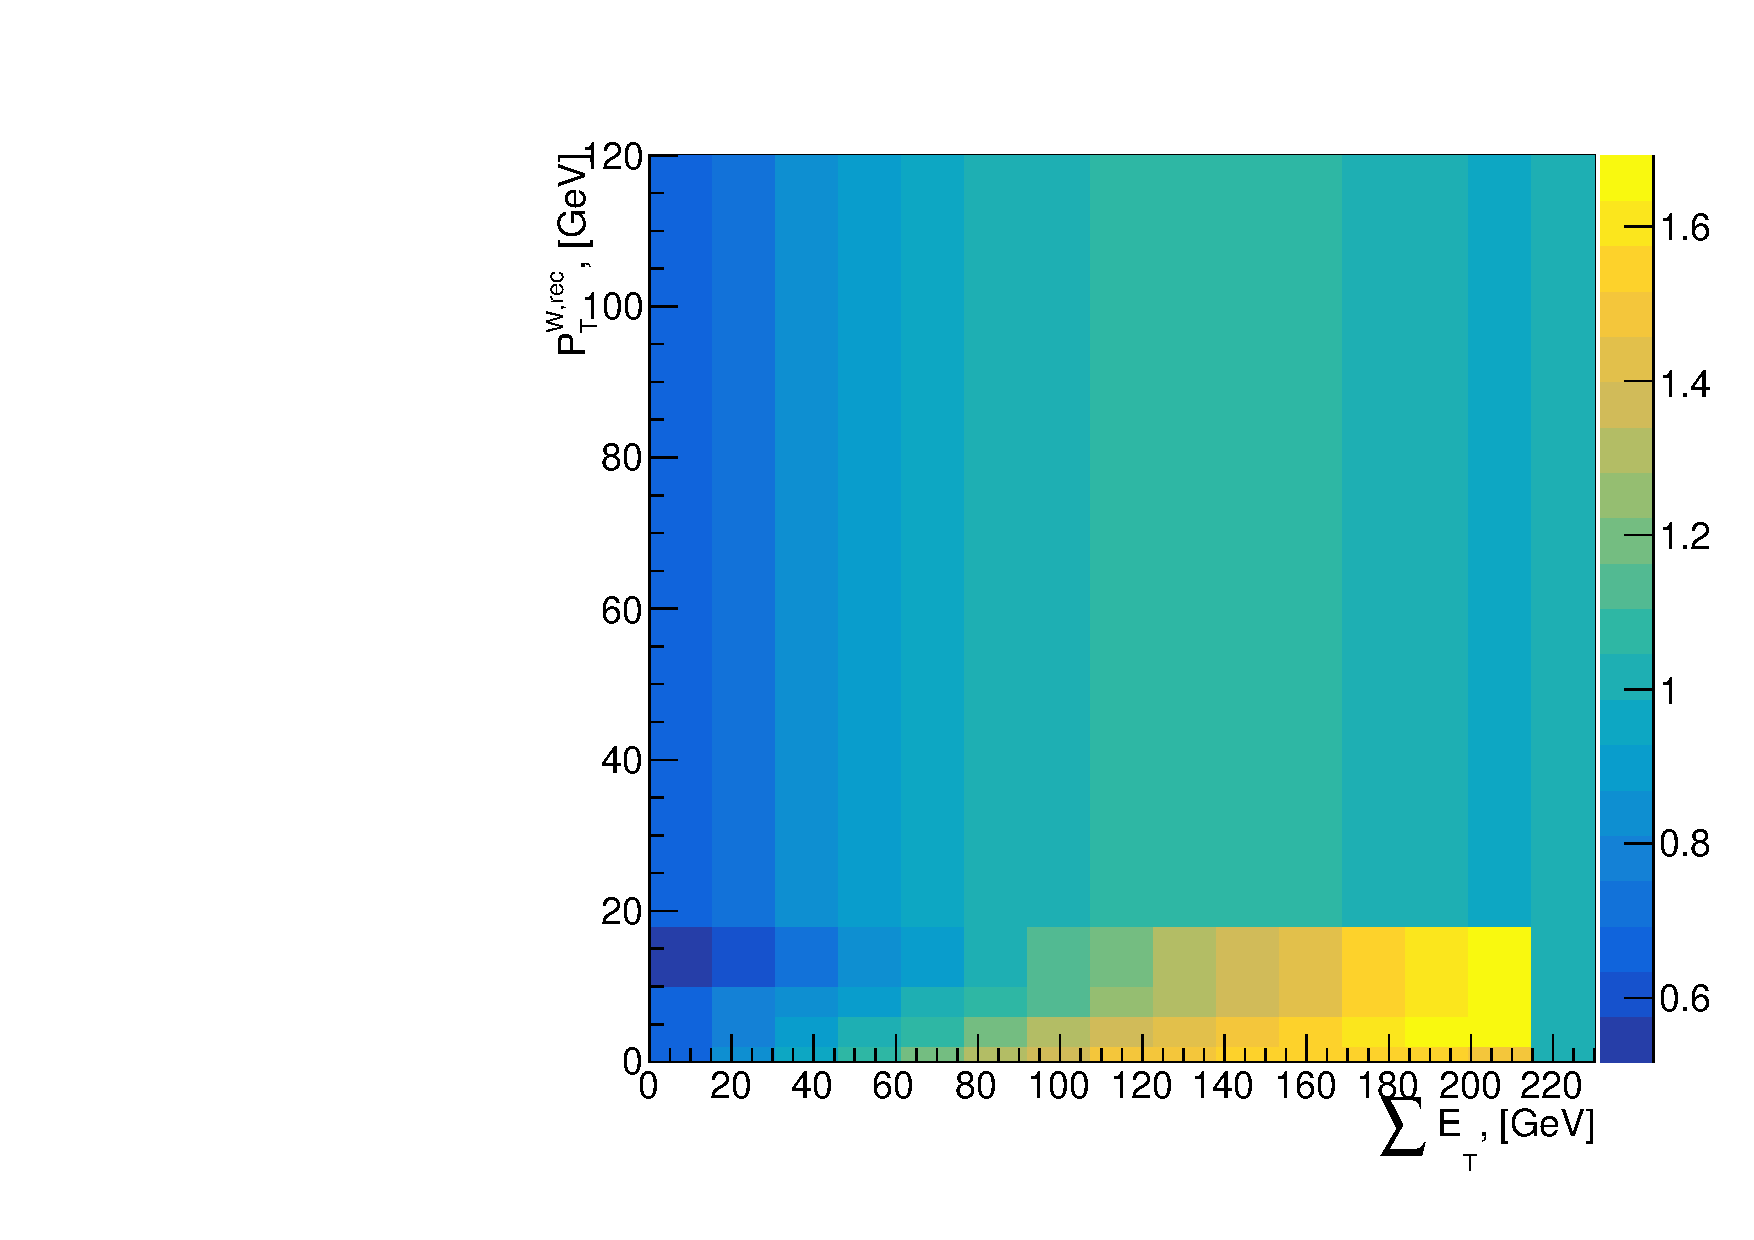
\includegraphics[width=1.\linewidth]{HadronRecoil/ReweightingPolMP.pdf} \\ b)}
\end{minipage}
\caption{Distribution of \sumet reweighting constants derived for a) $W^{+} \to e \nu$ and b) $W^{+} \to \mu \nu$ MC sample using polynomial order 2 approximation.}
\label{ris:SumEtCorPol}
\end{figure}

\subsubsection{Statistical error estimation}

Statistical error on the \sumet reweigting is estimated using Toy MC method, described in Chap.\ref{chap:Unc} from the polynomial order 2 approximation. The fitted parameters of the polynomials are varied inside each $p_T^{W, rec}$ bin within their fit uncertainties as in Eq. \ref{eq:ToyMethod}. Because of the possible correlations between fitted parameters, the multivariate Gaussian distribution have been used, that is calculated as:
\begin{equation}
p(x;\mu, \Sigma) =\frac{1}{(2\pi)^{n/2}|\Sigma|^{1/2}} exp\Big(-\frac{1}{2}(x-\mu)^{T}\Sigma^{-1}(x-\mu)\Big),
\end{equation}
where $\mu\in \boldsymbol{R}^{n}$ are the obtained from the fit paremeters and $\Sigma$ is $n \times n$ covariance matrix of these parameters. In case of the polynomial order two n=3. For statistic error determination total number of 25 toys have been used. Total error is calculated using Eq.\ref{eq:ToyError}.

\subsubsection{Effect of the \sumet correction on cross-section}

Overall effect of the \sumet correction for different methods is summarised in Tab. \ref{SumetCW}. Statistical error, estimated using Toy MC method is negligible.  Sign of the effect differs for different W channels, that cannot be explained by a systematic error coming from the method. This effect also cannot be explained from a physical point of view, so it was decided not to use this corrections in a final analysis.

 \begin{table}
 \caption{Effect of \sumet correction on a $C_{W}$ for a different channels and methods}
\label{SumetCW}
\begin{center}
\begin{tabular}{c | c | c |  c |  c   }
\hline
Channel & $\delta C_W$ & $\delta C_W$ & $\delta C_W$ & $\delta C_W$ \\
& no approximation & polynomial order 2 & polynomial order 1 & Toy MC \\
\hline
\hline
$W^{+} \to e^{+}\nu$ & &0.39\%  & 0.31\% & 0.03\% \\
$W^{-} \to e^{-}\nu$ & &0.33\%  & 0.22\% & 0.03\% \\
$W^{+} \to \mu^{+}\nu$ & &-0.20\%  & -0.28\% & 0.03\% \\
$W^{-} \to \mu^{-}\nu$ & &-0.21\%  & -0.27\% & 0.03\% \\
\hline
\end{tabular}
\end{center}

\end{table}


\subsection{Resolution corrections using Z events}\label{sec:ZperpSmear}
Another way to check resolution effects is to study \uperp and \upar  $ - p_T^{Z}$ distributions in events containing Z boson. This correction assumes, that any resolution mismodelling reflects discrepancies in the \sumet distribution, while the difference in the resolution at a given \sumet is subleading. There is a clear difference in an RMS of these distributions between data and MC, that cannot be accounted for a statistical uncertainties in the data (Fig. \ref{HadrRecoil:UparSmear} and Fig. \ref{HadrRecoil:UpeprSmear}). The difference in resolutions is consistent for \uperp and \upar $- p_T^{Z}$ distributions, but depends on an analysis channel and isolation + identification criteria.  

The resolution is corrected by smearing with a Gaussian distribution each component of a hadronic recoil:

\begin{equation}
\upar' = \upar+Gaus(0, d\sigma)
\end{equation}
\begin{equation}
\uperp' = \uperp + Gaus(0, d\sigma),
\end{equation}
where $d\sigma$ is a difference in a resoultions calculated as:
\begin{equation}
d\sigma=\sqrt{\sigma_{data}^2-\sigma_{MC}^2}
\end{equation}
Systematic error of this $d\sigma$ is taken as an statistical error for $\sigma_{data}$. Due to a random nature of this correction, effect is not stable for a small $d\sigma$. Systematic error have been estimated by repeating correction on the same sample 40 times. Overall sytematics effect is below 0.2\% for each channel (Tab. \ref{SmearCW}).
\begin{figure}[!tbp]
\begin{minipage}[h]{0.32\linewidth}
\center{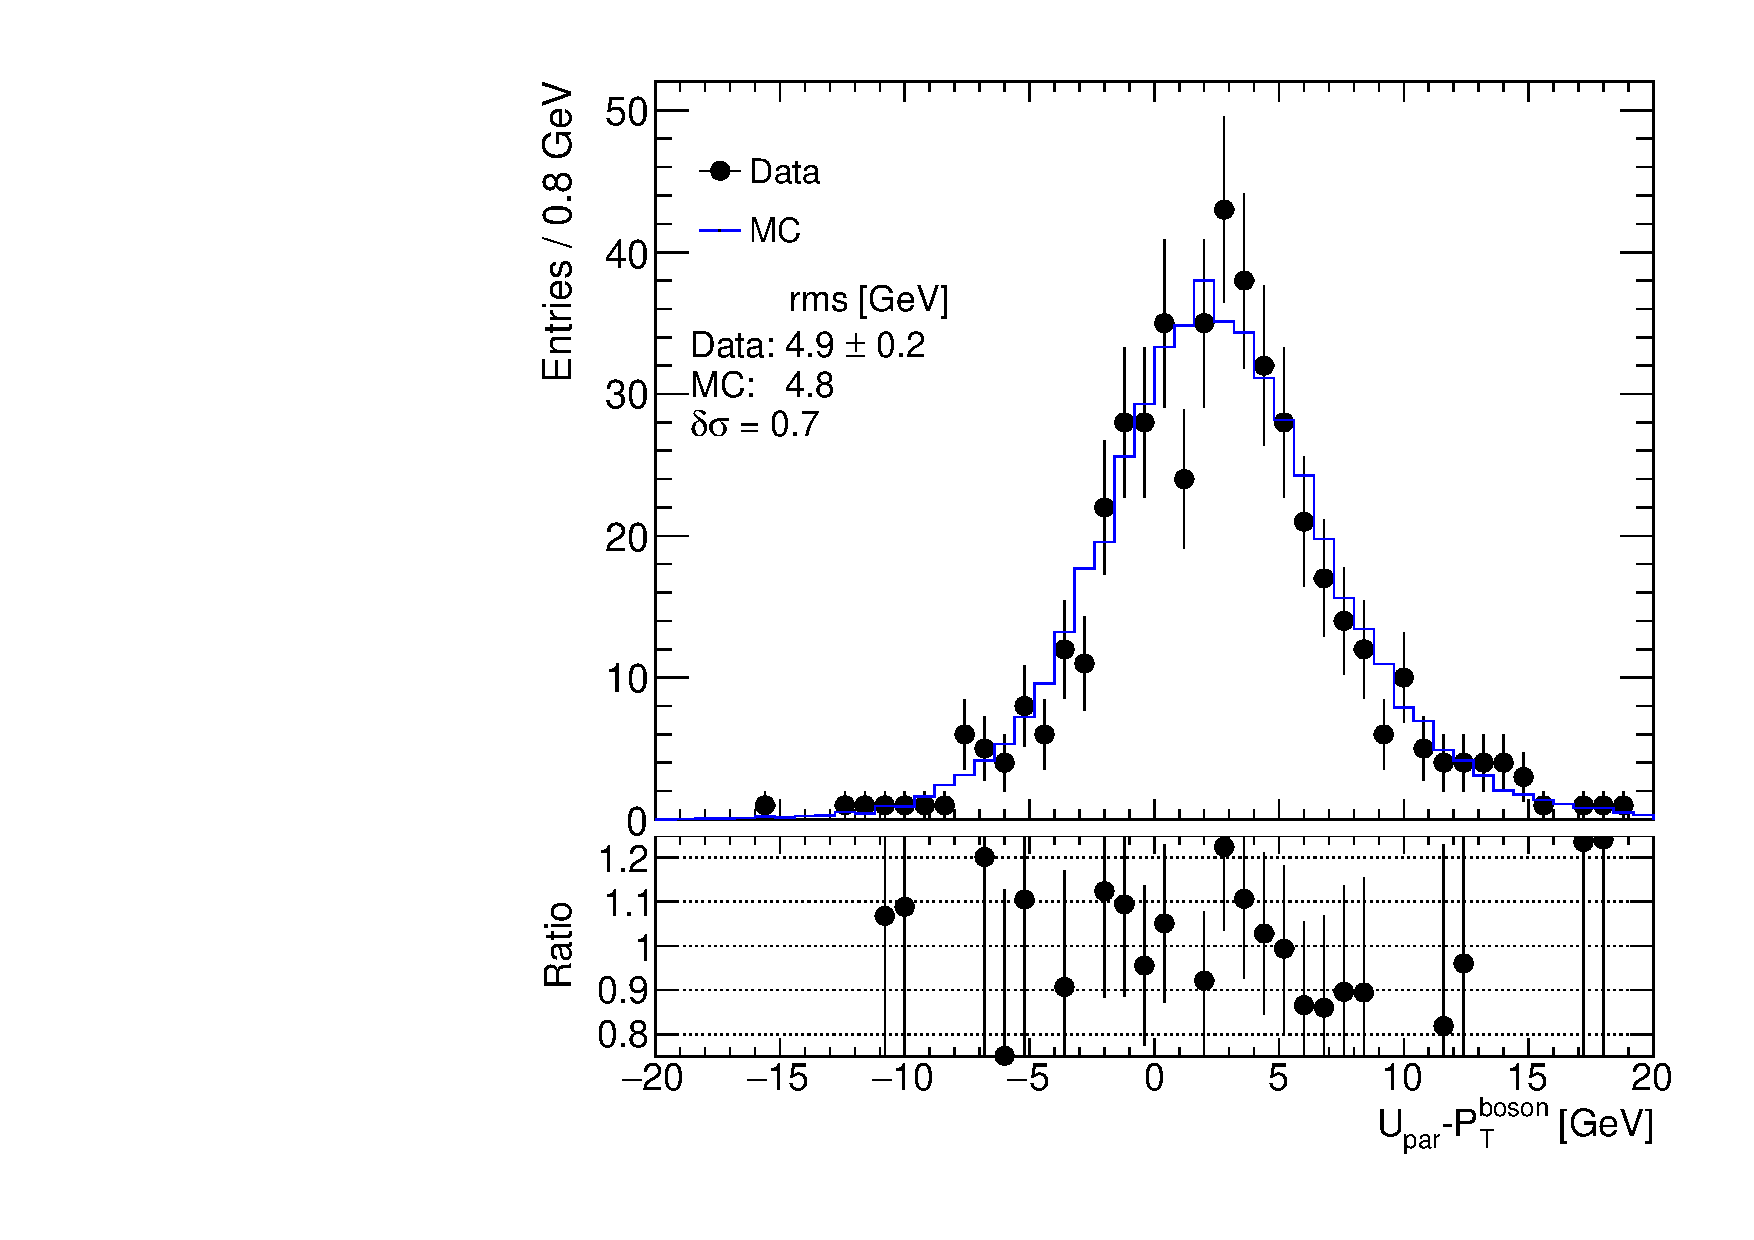
\includegraphics[width=1.\linewidth]{HadronRecoil/UParERMS.pdf} \\ a)}
\end{minipage}
\hfill
\begin{minipage}[h]{0.32\linewidth}
\center{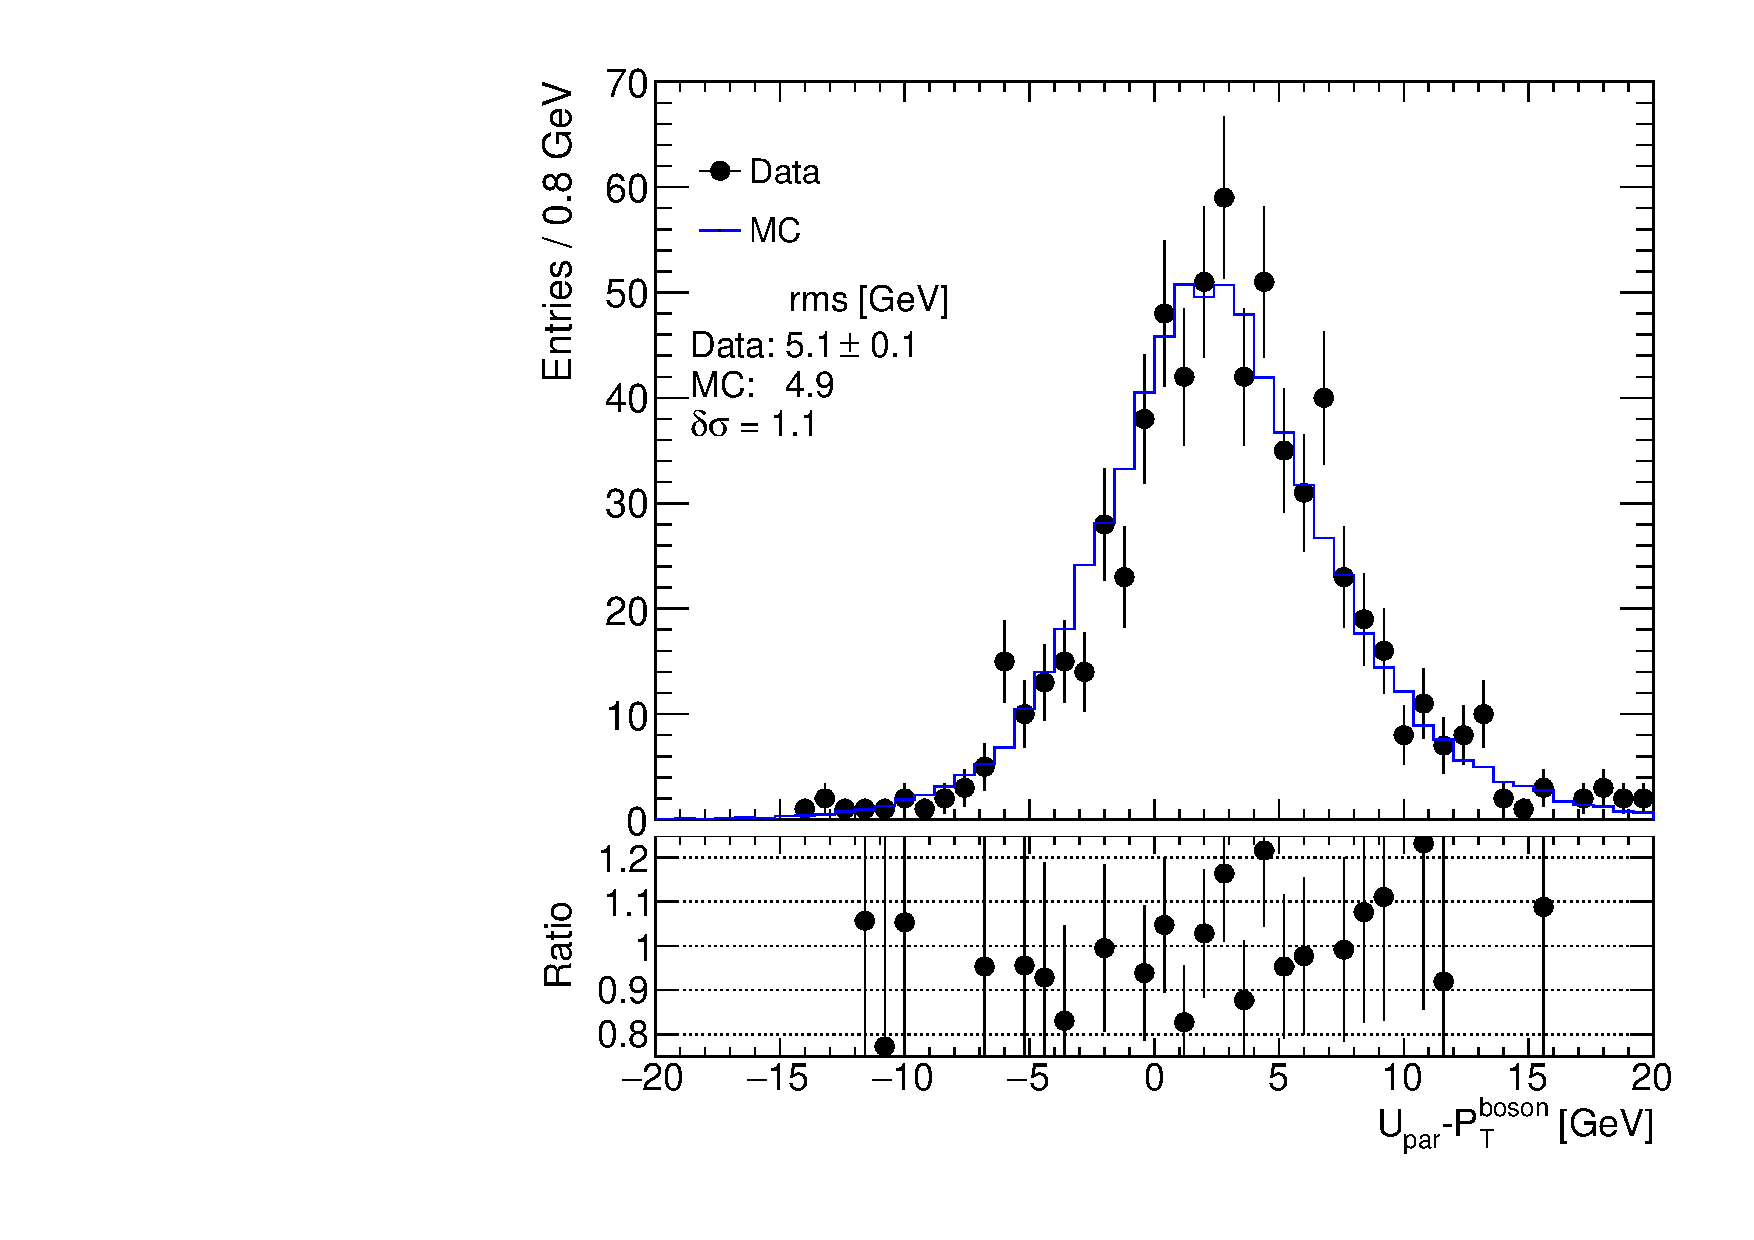
\includegraphics[width=1.\linewidth]{HadronRecoil/UParMRMS.pdf} \\ b)}
\end{minipage}
\hfill
\begin{minipage}[h]{0.32\linewidth}
\center{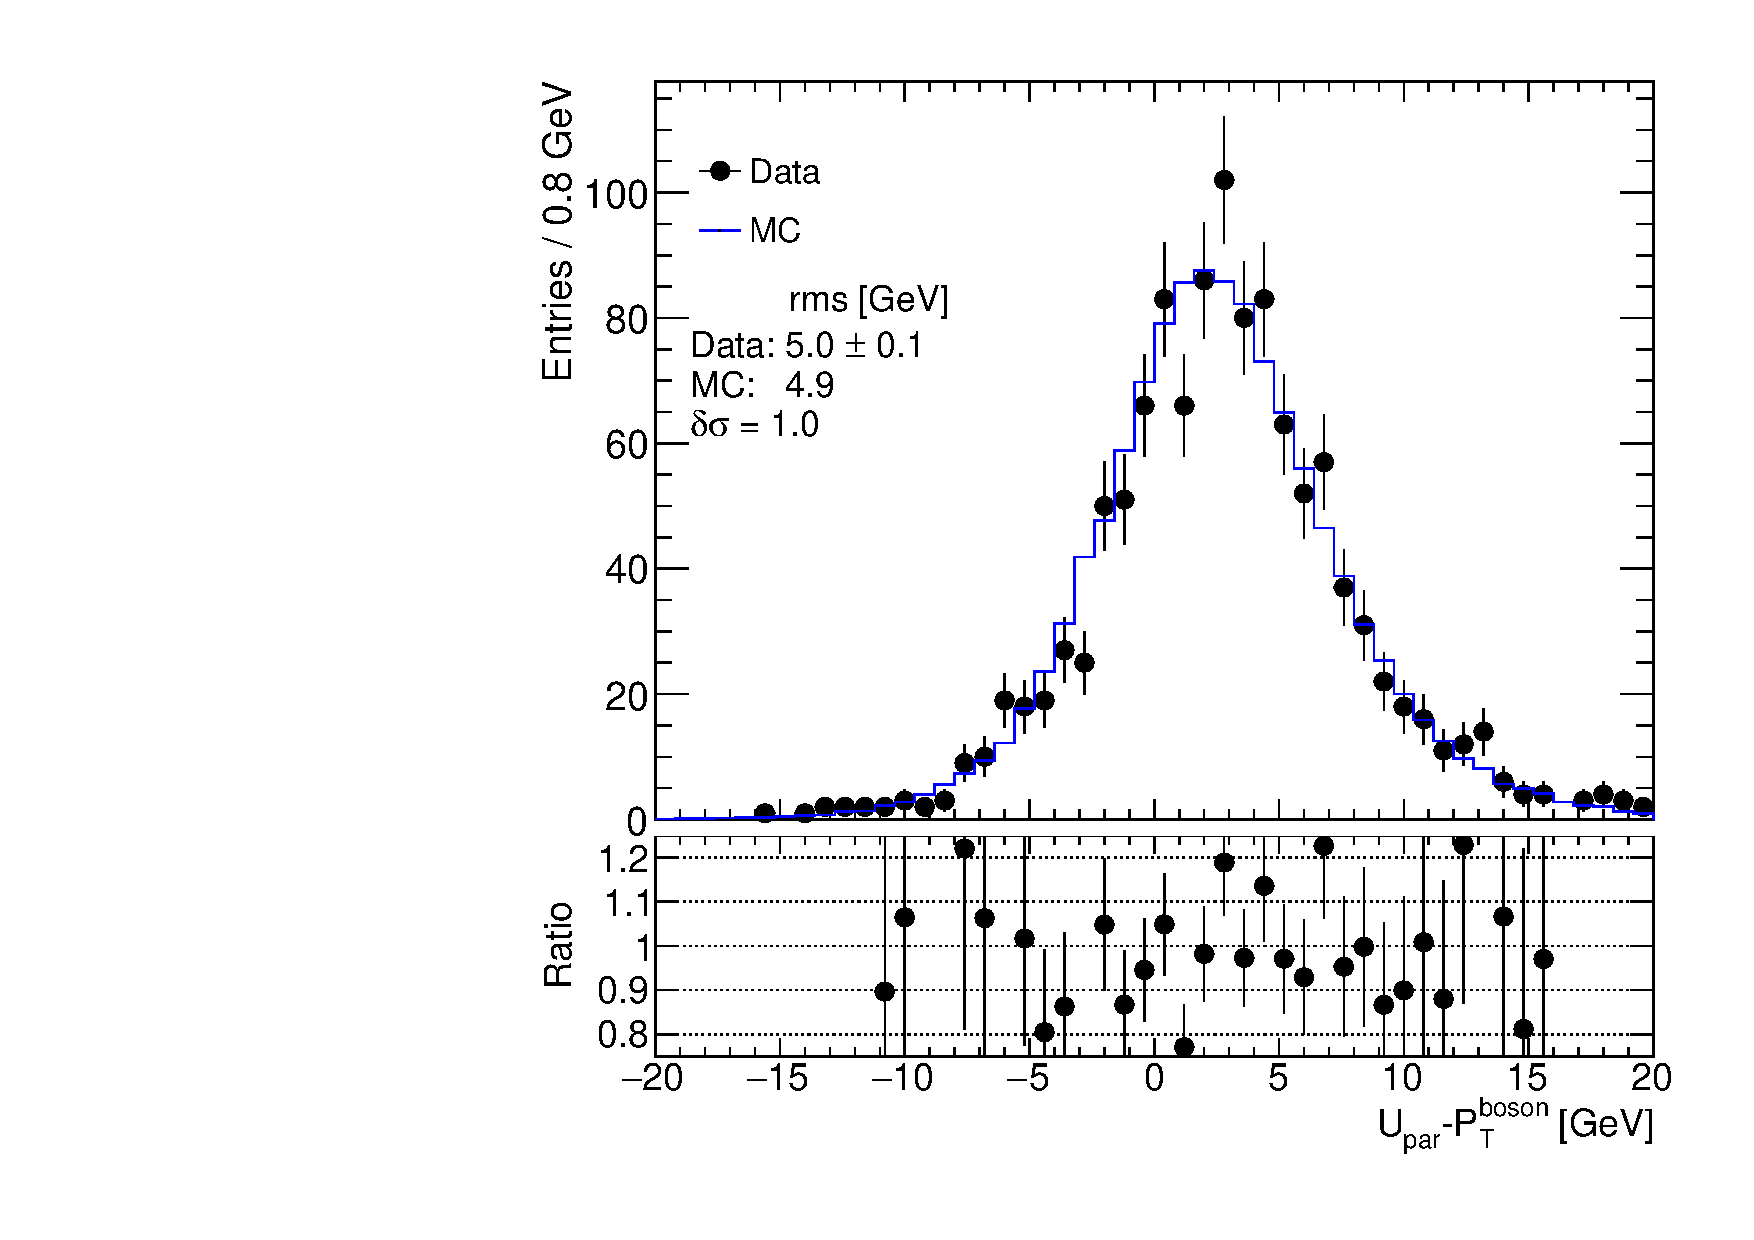
\includegraphics[width=1.\linewidth]{HadronRecoil/UParTotalRMS.pdf} \\ c)}
\end{minipage}
\caption{Parallel hadronic recoil component distribuiton from a) the $Z\to ee$ selection b) $Z\to\mu\mu$ selection and c) $Z\to ll$ selection. The expected contribution from signal is estimated with Monte Carlo simulation, other background sources are considered negligible.}
\label{HadrRecoil:UparSmear}
\end{figure}

\begin{figure}[!tbp]
\begin{minipage}[h]{0.32\linewidth}
\center{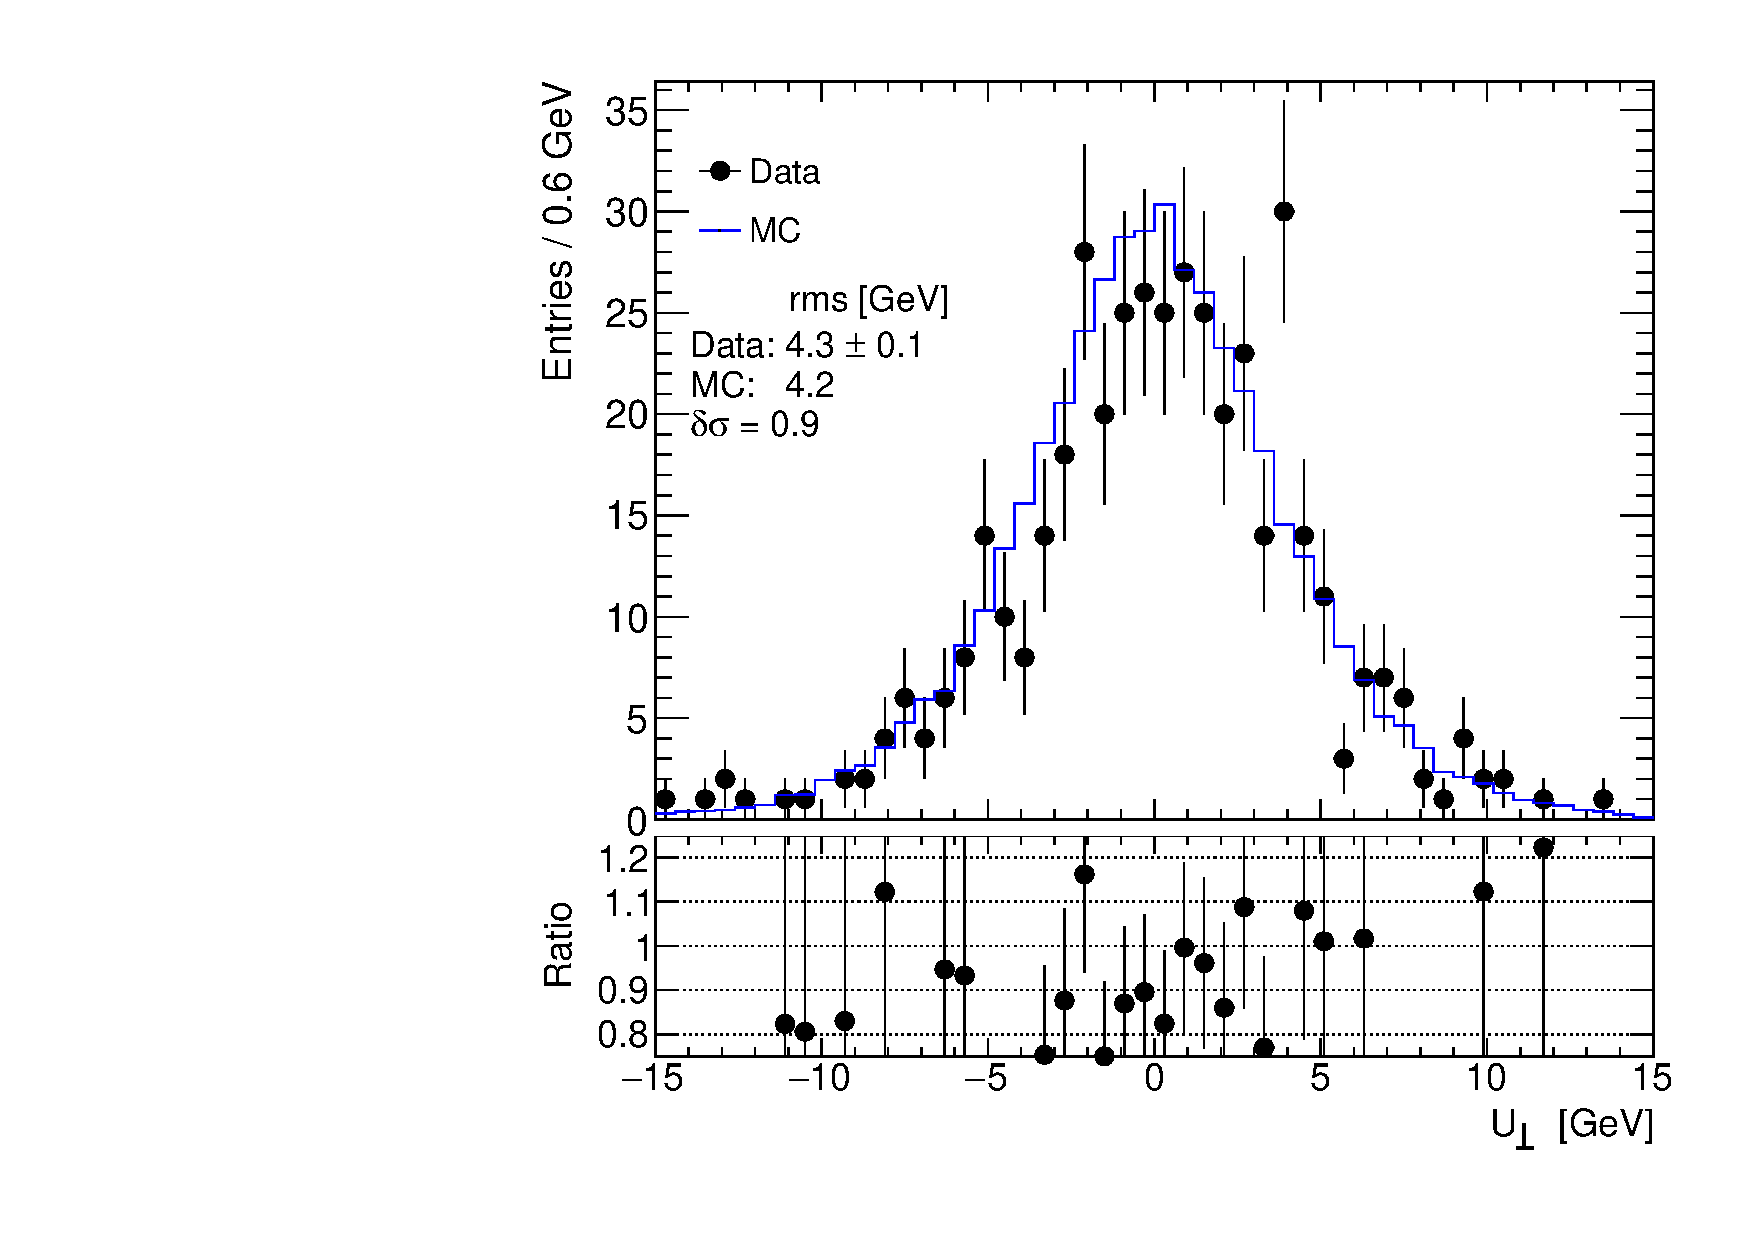
\includegraphics[width=1.\linewidth]{HadronRecoil/UPerpERMS.pdf} \\ a)}
\end{minipage}
\hfill
\begin{minipage}[h]{0.32\linewidth}
\center{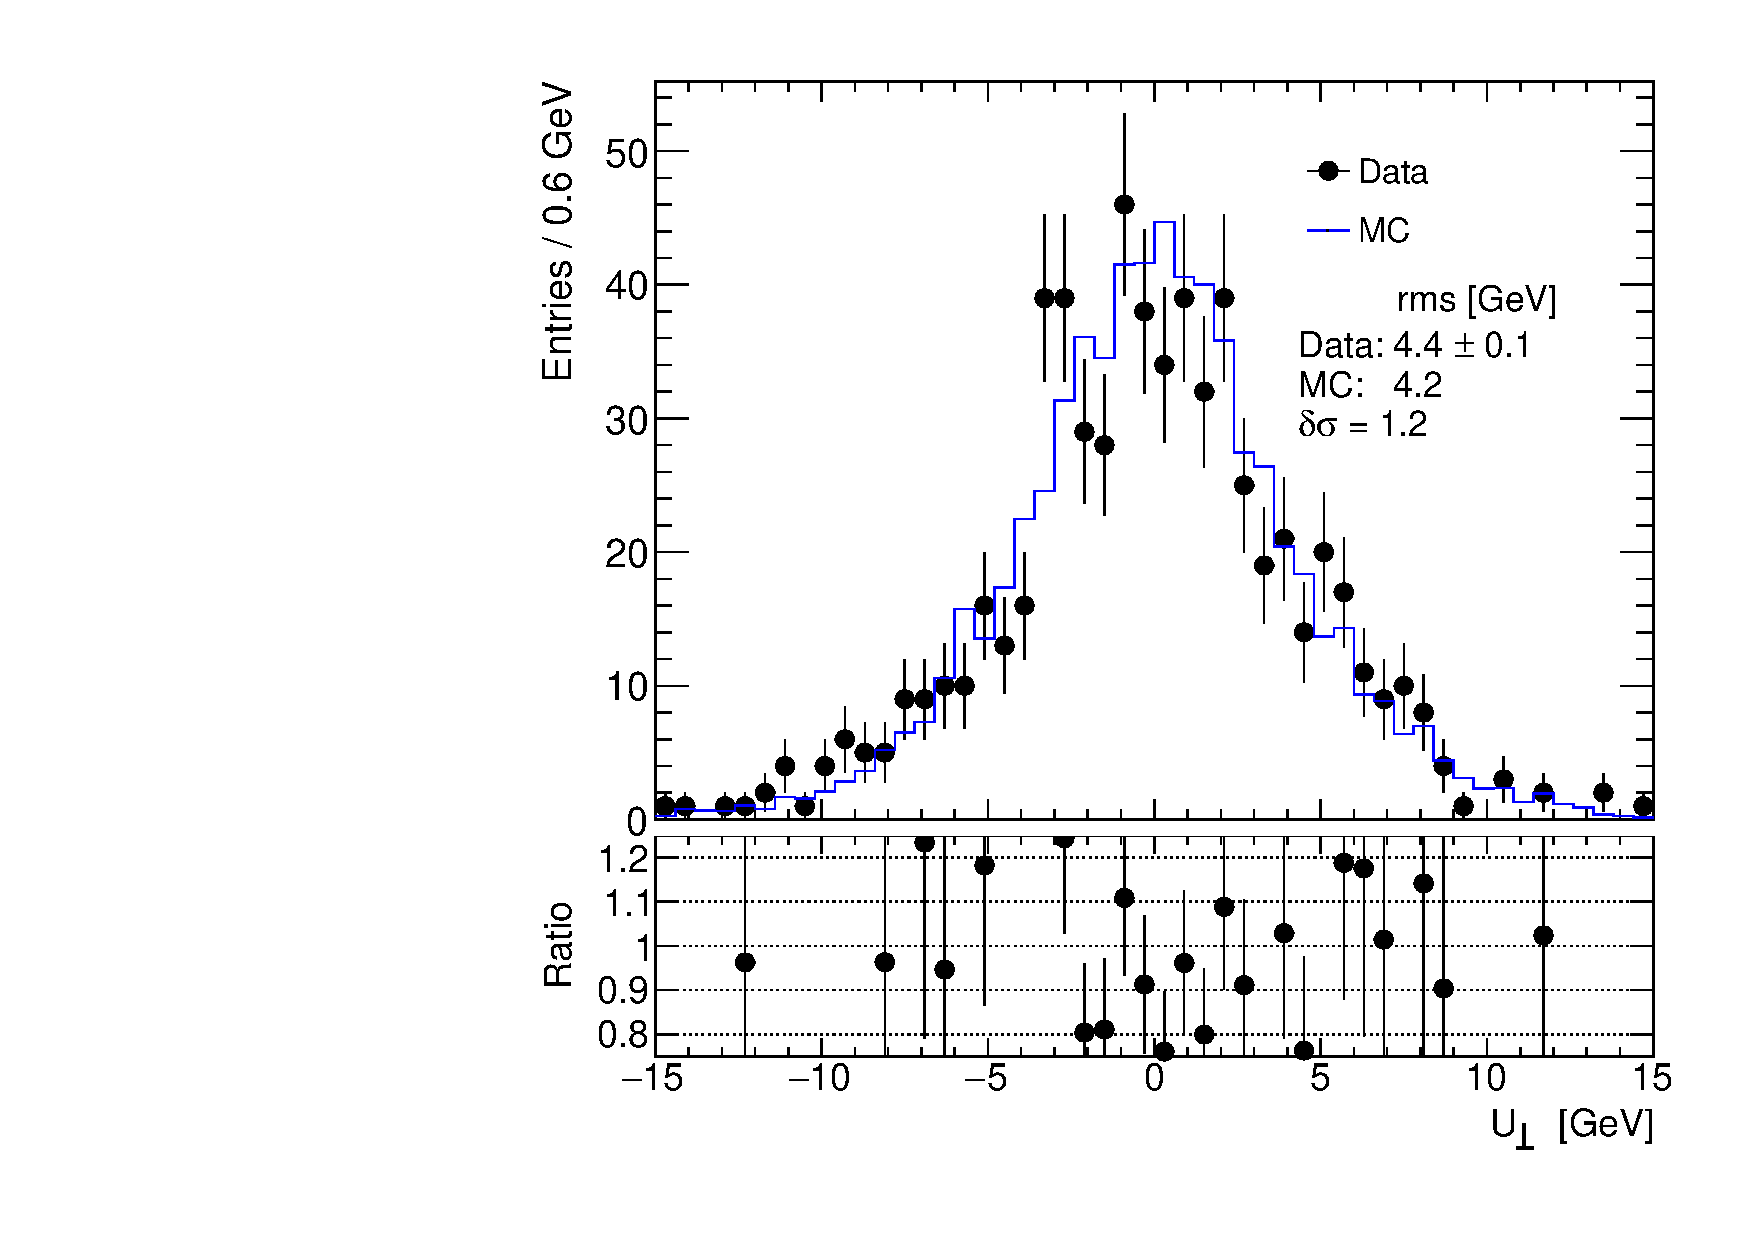
\includegraphics[width=1.\linewidth]{HadronRecoil/UPerpMRMS.pdf} \\ b)}
\end{minipage}
\hfill
\begin{minipage}[h]{0.32\linewidth}
\center{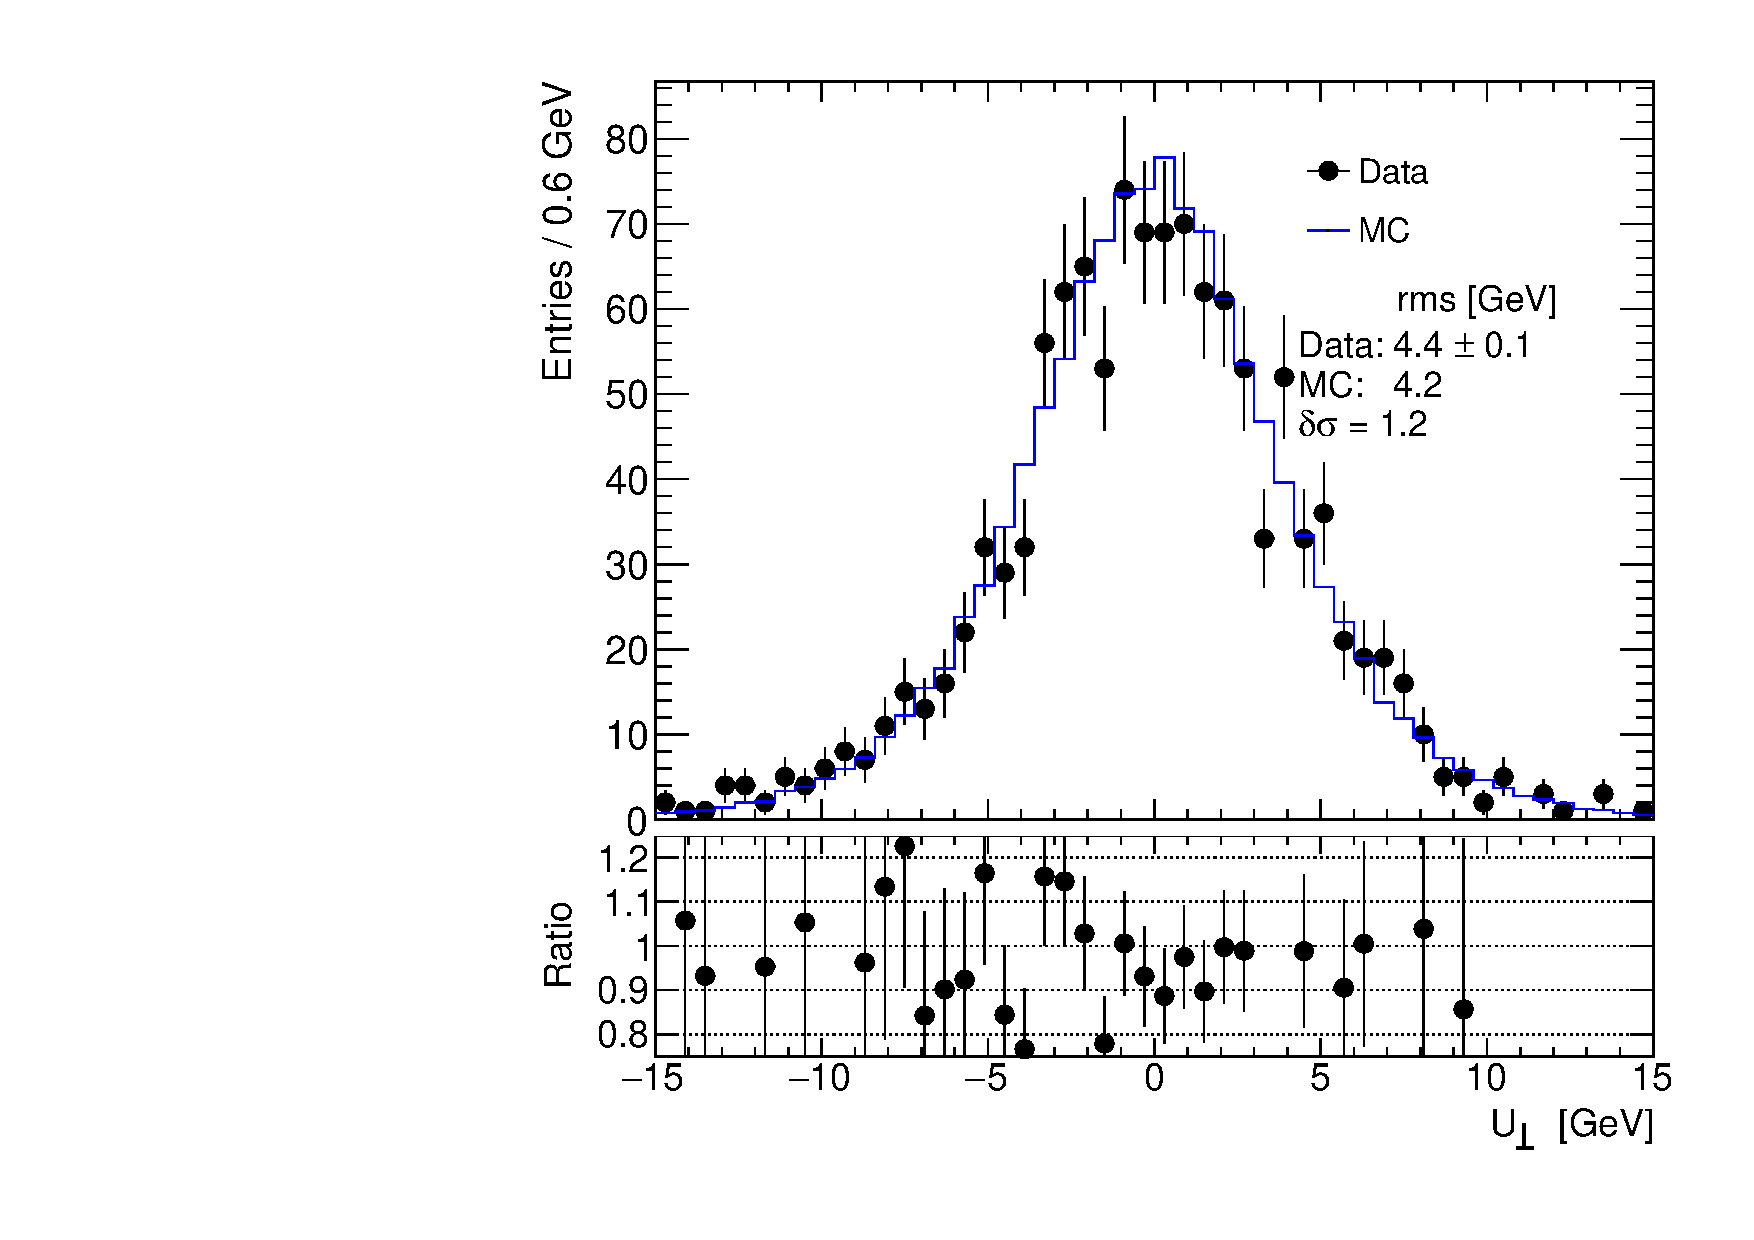
\includegraphics[width=1.\linewidth]{HadronRecoil/UPerpTotalRMS.pdf} \\ c)}
\end{minipage}
\caption{Perpendicular hadronic recoil component distribuiton from a) the $Z\to ee$ selection b) $Z\to\mu\mu$ selection and c) $Z\to ll$ selection. The expected contribution from signal is estimated with Monte Carlo simulation, other background sources are considered negligible.}
\label{HadrRecoil:UpeprSmear}
\end{figure}

 \begin{table}[!tbp]
 \caption{Effect of smearing correction on a $C_{W}$ for a different channels}
\label{SmearCW}
\begin{center}
\begin{tabular}{| l  | c | c | }
\hline
Channel & $\delta C_W$ & error \\
\hline
\hline
$W^{+} \to e^{+}\nu$ & -0.20\% & 0.04\% \\
$W^{-} \to e^{-}\nu$ & -0.11\% &  0.06\% \\
$W^{+} \to \mu^{+}\nu$ & -0.16\% & 0.04\% \\
$W^{-} \to \mu^{-}\nu$ & -0.12\% & 0.07\% \\
\hline
\end{tabular}
\end{center}

\end{table}

\section{Hadronic recoil bias correction}
As it was mentioned before, it is possible to use both Z and W boson samples for the hadronic recoil bias determination. Correction factor $HR_{SF}$ is applied as:
\begin{equation}
\upar^{MC,cor}=\upar^{MC} \cdot HR_{SF}
\end{equation}
and can be obtained by scanning the impact of the scaling factor on the data to MC agreement of the distributions that are dominated by the recoil scale uncertainties.  The best correction factor and it's error is obtained from the fit of \chiD distributions with the function:
\begin{equation}\label{eq:chiD}
\chi^2 = \frac{(HR_{SF}-sf_{best})^2}{\sigma_{sf}^2}+\chi^2_0,
\end{equation}
where $sf_{best}$ is the best scale factor,  $\sigma_{sf}$ is a statistical error of this parameter and $\chi^2_0$ is a value of \chiD in a minimum. 

This procedure can be used in both Z and W boson samples.
\subsection{Bias determination from \mtw distribution}
\begin{figure}[!tbp]
\minipage{0.32\textwidth}
  \center{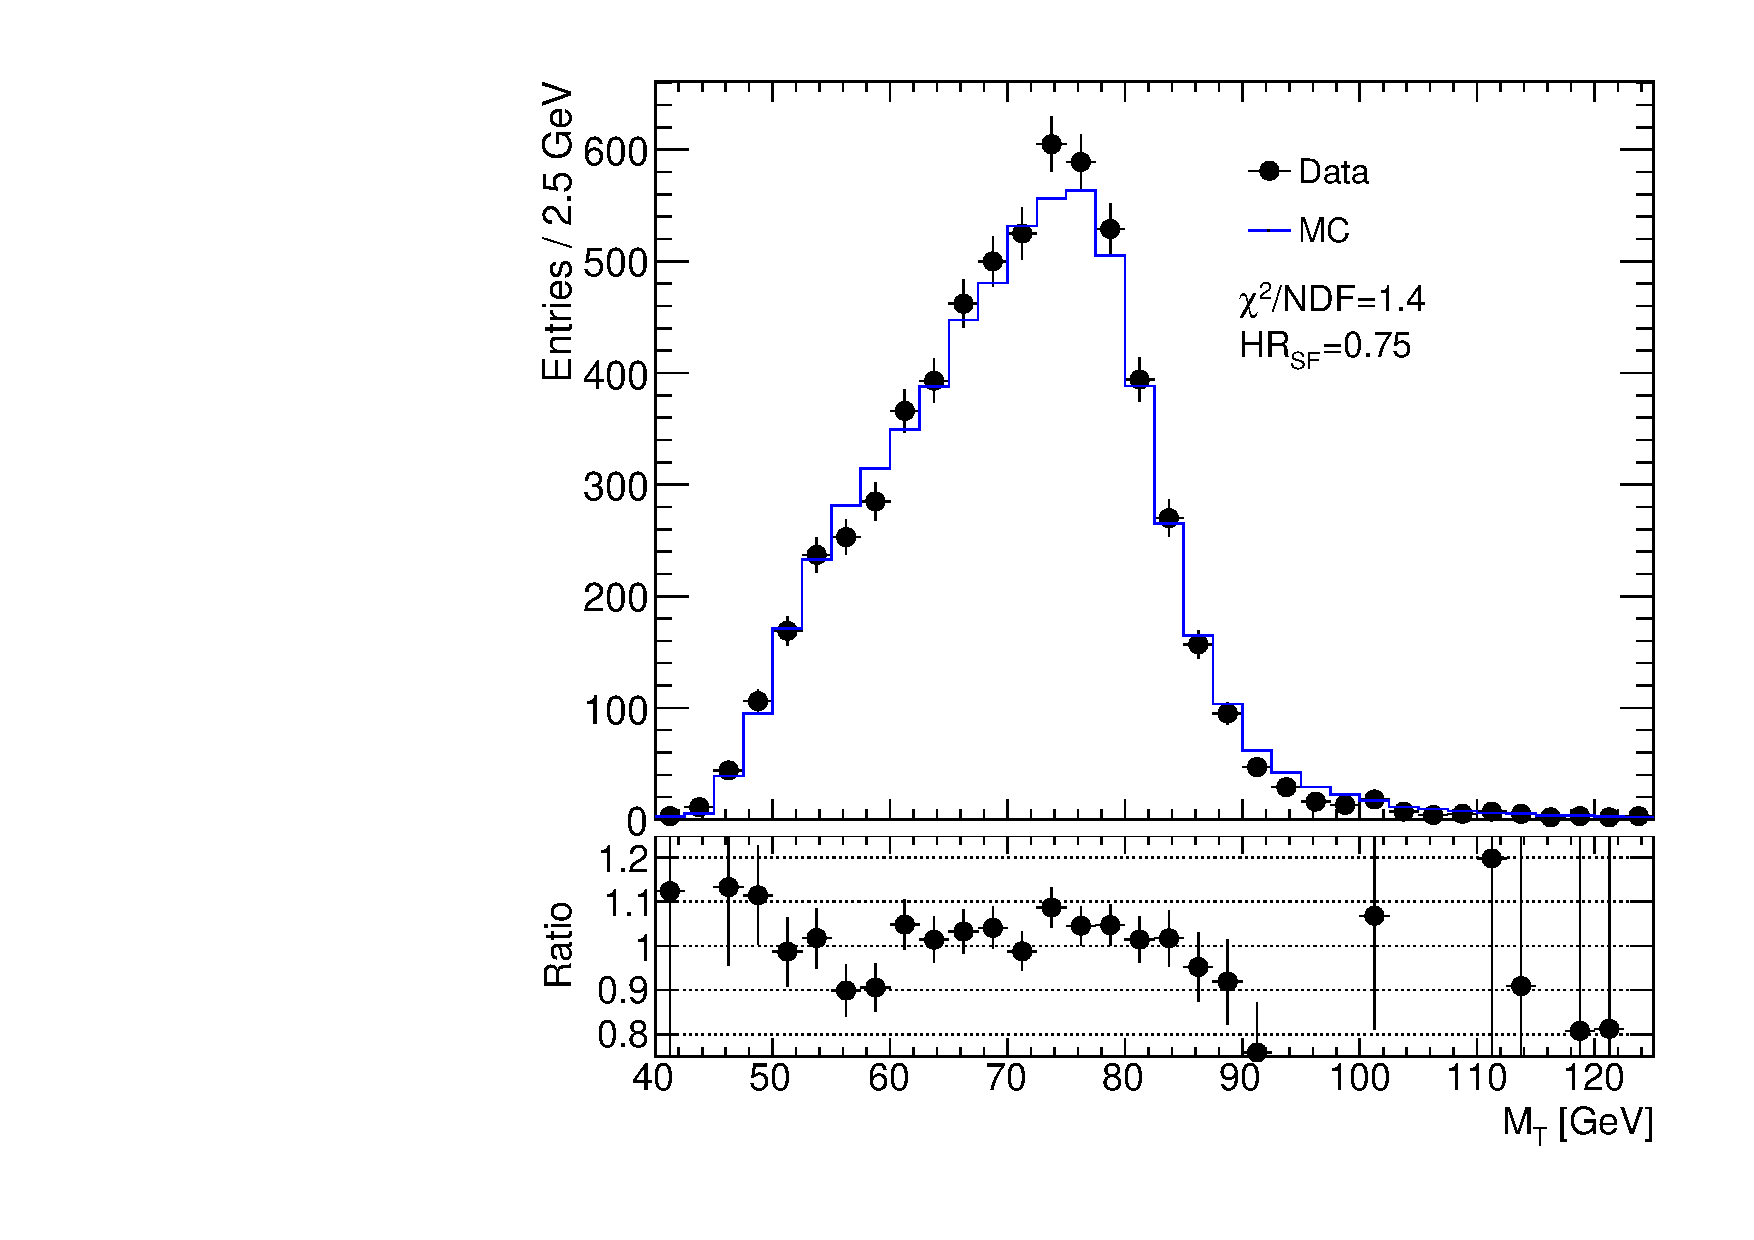
\includegraphics[width=\linewidth]{HadronRecoil/MtWEScale0.pdf} a)}
\endminipage\hfill
\minipage{0.32\textwidth}
   \center{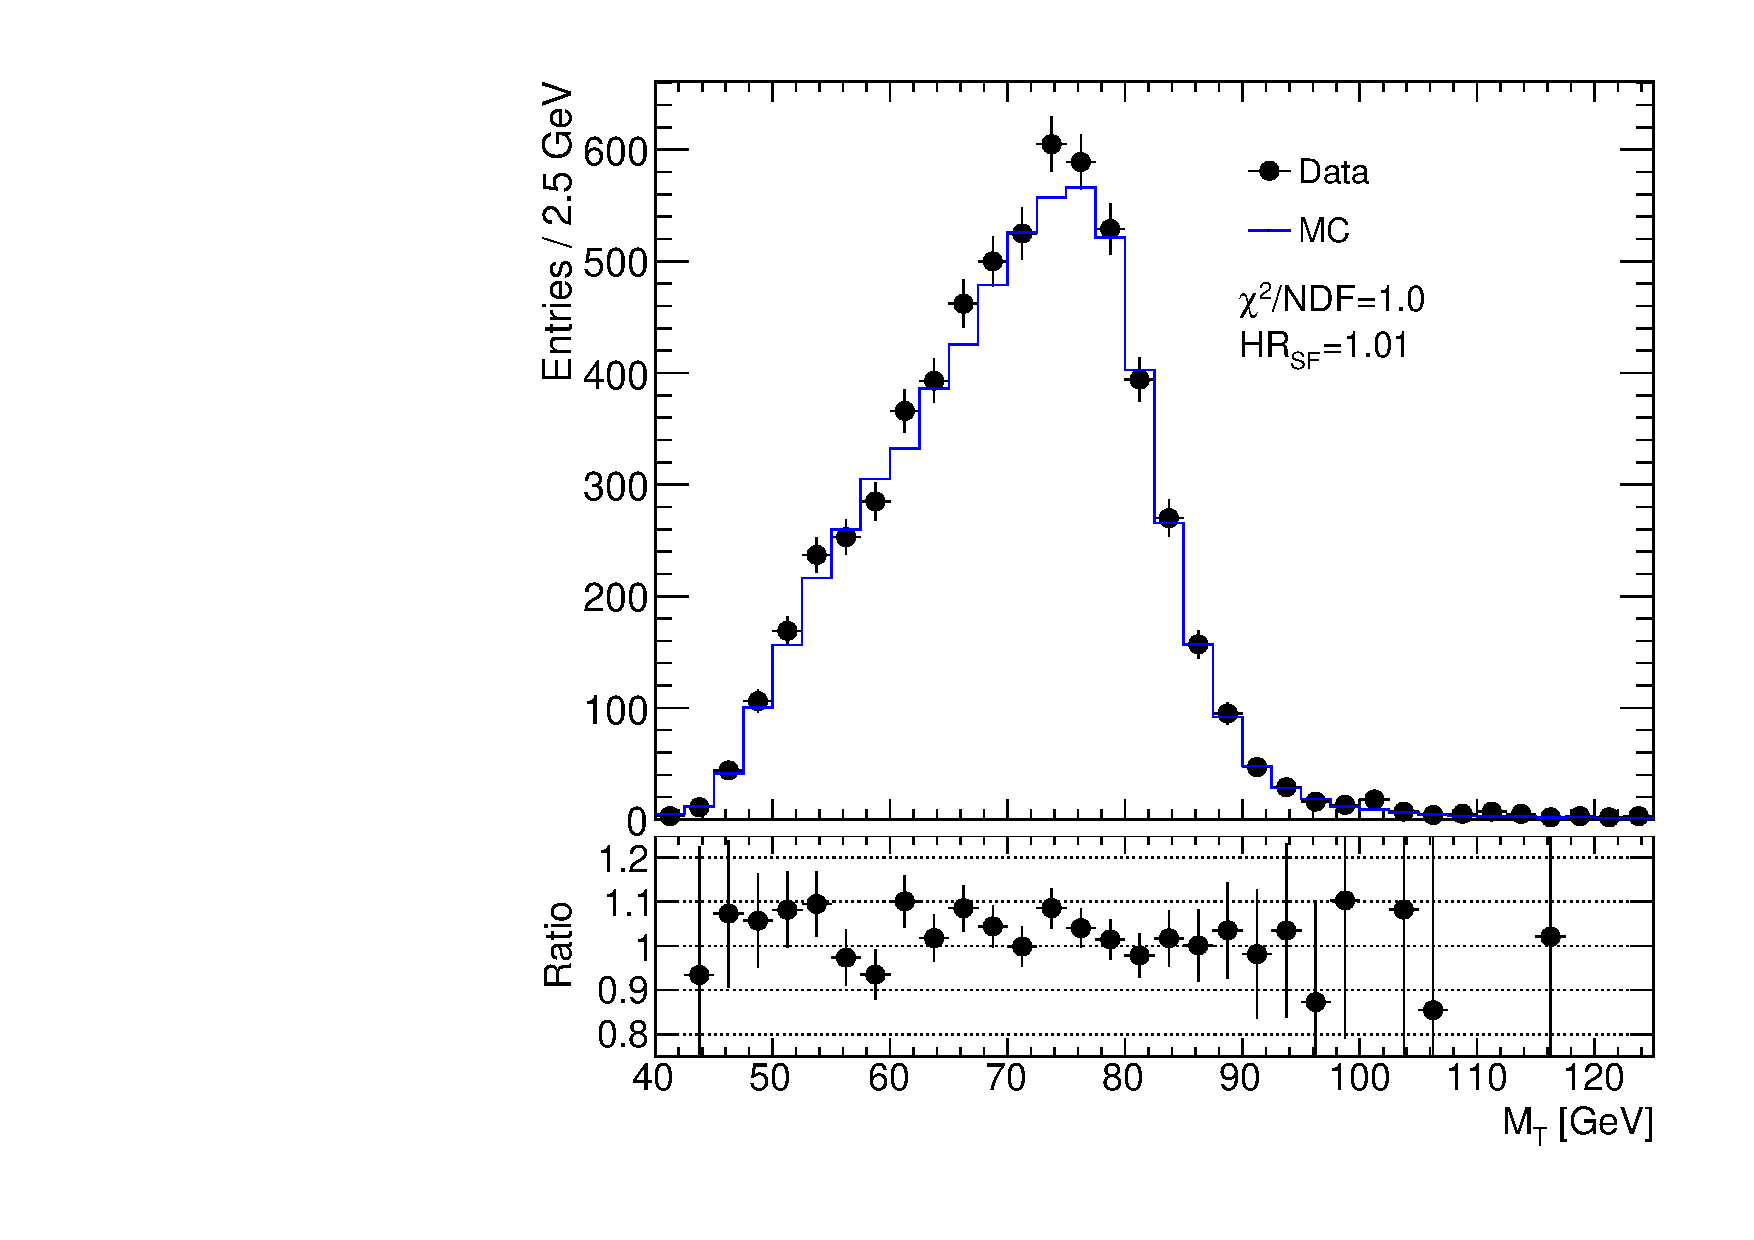
\includegraphics[width=\linewidth]{HadronRecoil/MtWEScale13.pdf} b)}
\endminipage\hfill
\minipage{0.32\textwidth}%
   \center{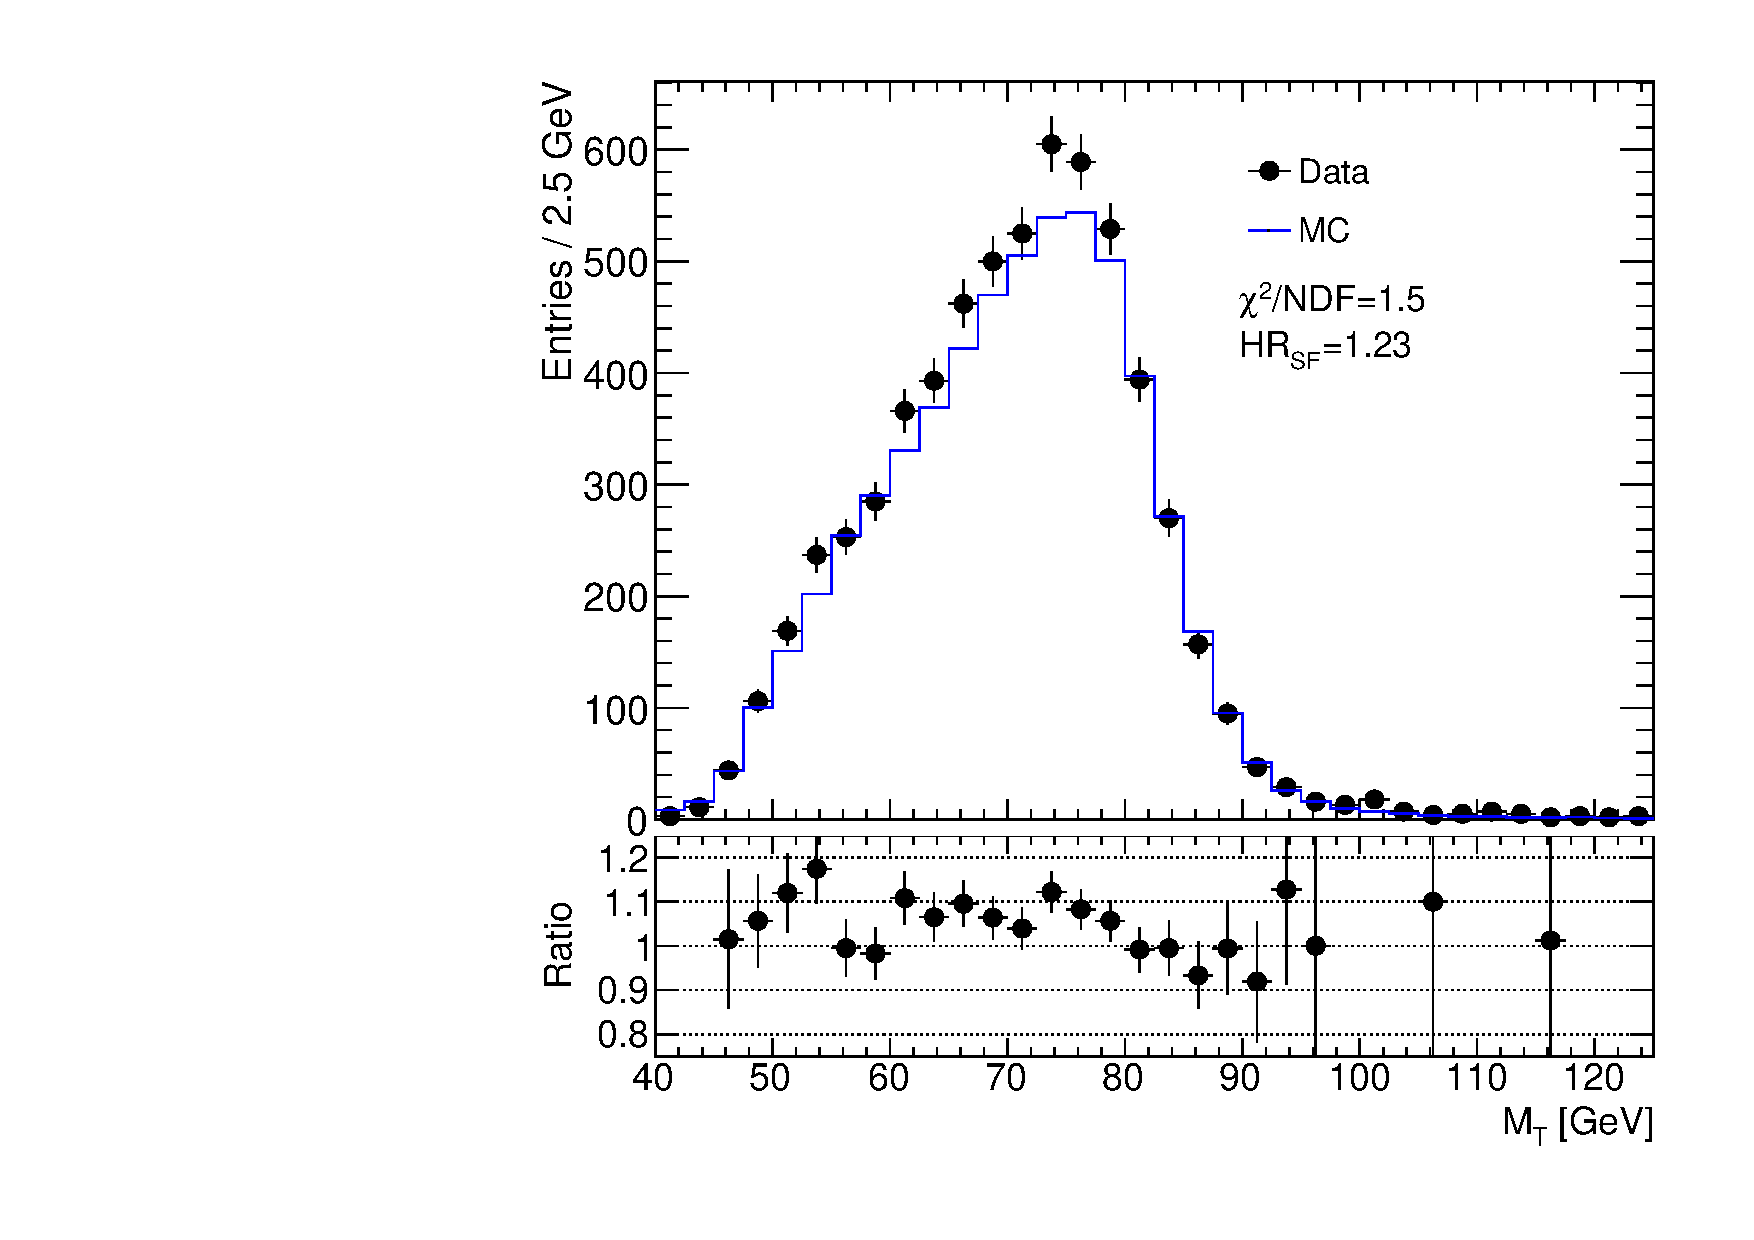
\includegraphics[width=\linewidth]{HadronRecoil/MtWEScale24.pdf} c)}
\endminipage
\caption{Mass transverse distribution from the \wenu selection for different hadronic recoil scales: a) $HR_{SF}$=0.75 b) $HR_{SF}$= 1.1 c) $HR_{SF}$=1.23. The expected contributions from signals and backgrounds are estimated with Monte Carlo simulation, except for a QCD background, that is not included.}
\label{HadronRecoilScaleMtW}
\end{figure}

Since the W boson transverse momentum cannot be measured in two different ways in order to provide the reference for a hadronic recoil scale, determination of the hadronic recoil bias should use the distributions, that  are not sensitive to the truth \ptw spectrum.  One of the optimal choises is the \mtw distribution. The transverse mass distribution for a different scale choises is shown on a Fig. \ref{HadronRecoilScaleMtW}.The expected contributions from signals and backgrounds are estimated with Monte Carlo simulation, except for a multijet background, because its shape and number of events depends on a hadronic recoil scale and thus needs to be recalculated for each value of $HR_{SF}$. 

\begin{figure}[!tbp]
\begin{minipage}[h]{0.49\linewidth}
\center{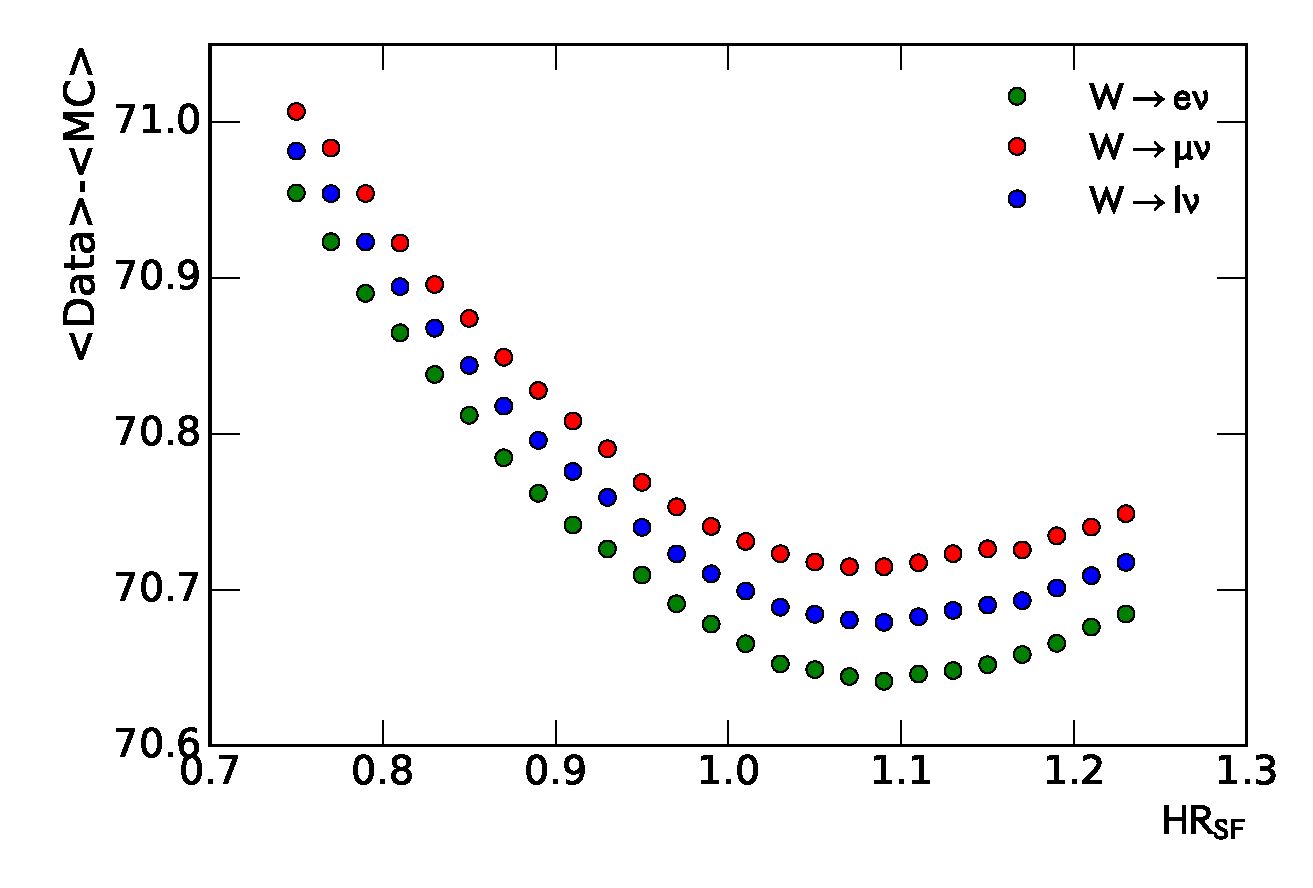
\includegraphics[width=1.\linewidth]{HadronRecoil/MeanAll.pdf} \\ a)}
\end{minipage}
\hfill
\begin{minipage}[h]{0.49\linewidth}
\center{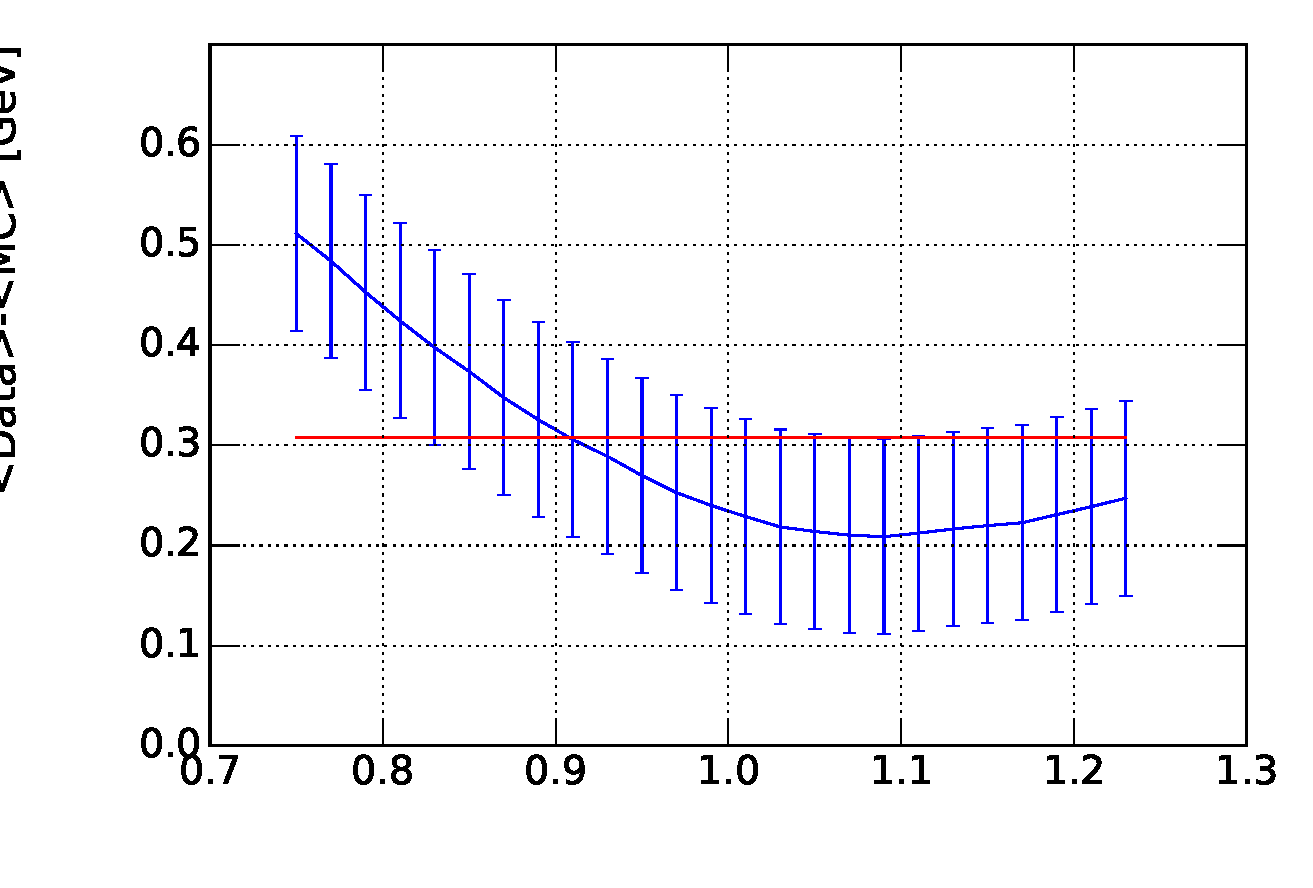
\includegraphics[width=1.\linewidth]{HadronRecoil/MeanCombined.pdf} \\ b)}
\end{minipage}
\caption{a) Distribution of difference in a mean transverse momentum $<\mtw>$ between data and MC as a function of hadronic recoil scale $HR_{SF}$ for different W boson channels. 
b) Distribution of difference in a mean transverse momentum $<\mtw>$ between data and MC as a function of hadronic recoil scale $HR_{SF}$ for combined $W \to l \nu$ selection. Errors for each point are calculated as a standard error of mean. Below red line are values of  $HR_{SF}$ within 1 $\sigma$ uncertainty. The expected contributions from signals and backgrounds are estimated with Monte Carlo simulation, except for a QCD background, that is not included.}
\label{fig:HRBiasMean}
\end{figure}

One of the possible ways to determine the correction factor is to use a difference in the mean of the transverse mass distributions in data and MC (Fig.~\ref{fig:HRBiasMean}). Statistical error on a correction factor is considered a dominating one and estimated as an standard error of mean $\sigma ( <\mtw> ) $, that is calculated as:
\begin{equation}
\sigma \Big( <\mtw> \Big) = \frac{\sigma( \mtw )}{\sqrt N},
\end{equation}
where $\sigma(\mtw)$ is a standard deviation of $\mtw$ distribution and N is a total number of events used. The minimum difference is obtained at $HR_{SF}=1.1\pm0.2$. The precision of this method is low, is it is mainly used as a cross-check of other methods. 

\begin{figure}[!tbp]
\begin{minipage}[h]{0.49\linewidth}
\center{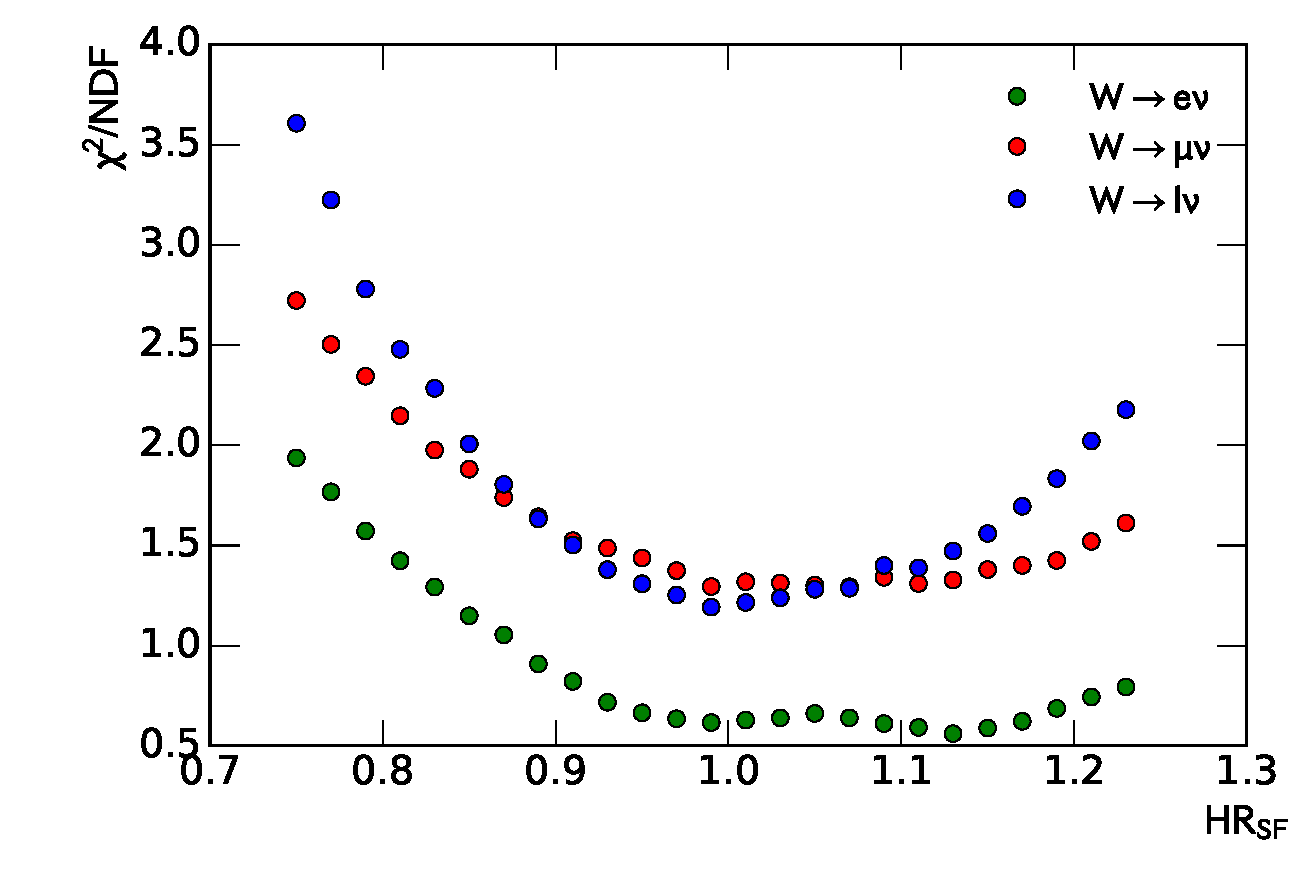
\includegraphics[width=1.\linewidth]{HadronRecoil/chi2AllChannelsMtw.pdf} \\ a)}
\end{minipage}
\hfill
\begin{minipage}[h]{0.49\linewidth}
\center{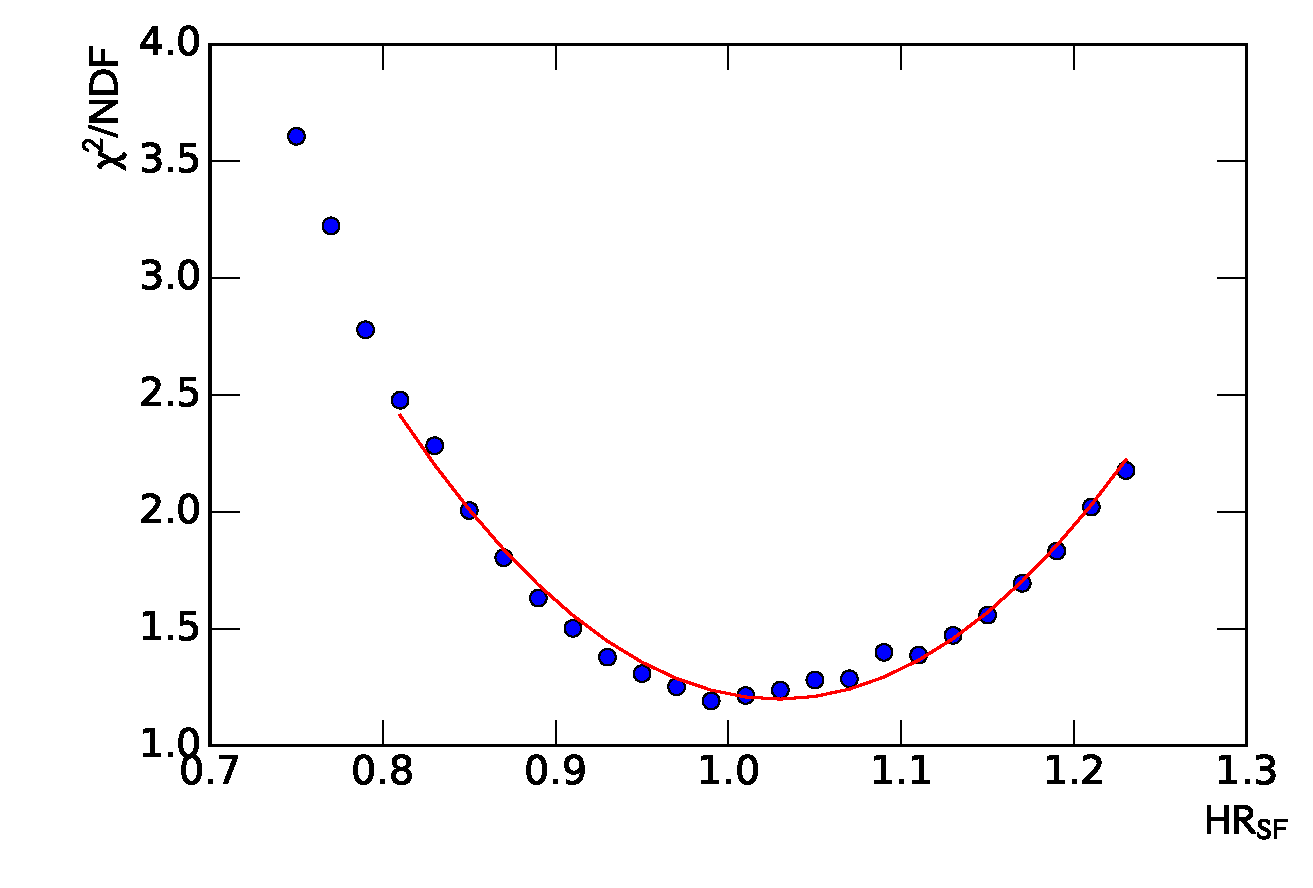
\includegraphics[width=1.\linewidth]{HadronRecoil/chi2TotalMtw.pdf} \\ b)}
\end{minipage}
\caption{a) Distribution of \chiD  between data and MC for transverse momentum $<\mtw>$ as a function of hadronic recoil scale $HR_{SF}$ for different W boson channels. 
b) Distribution of \chiD  between data and MC for transverse momentum $<\mtw>$ as a function of hadronic recoil scale $HR_{SF}$ for combined $W \to l \nu$ selection. Fit results are shown by a red line.The expected contributions from signals and backgrounds are estimated with Monte Carlo simulation, except for a QCD background, that is not included.}
\label{mtWChi2}
\end{figure}

\begin{figure}[!tbp]
\centering
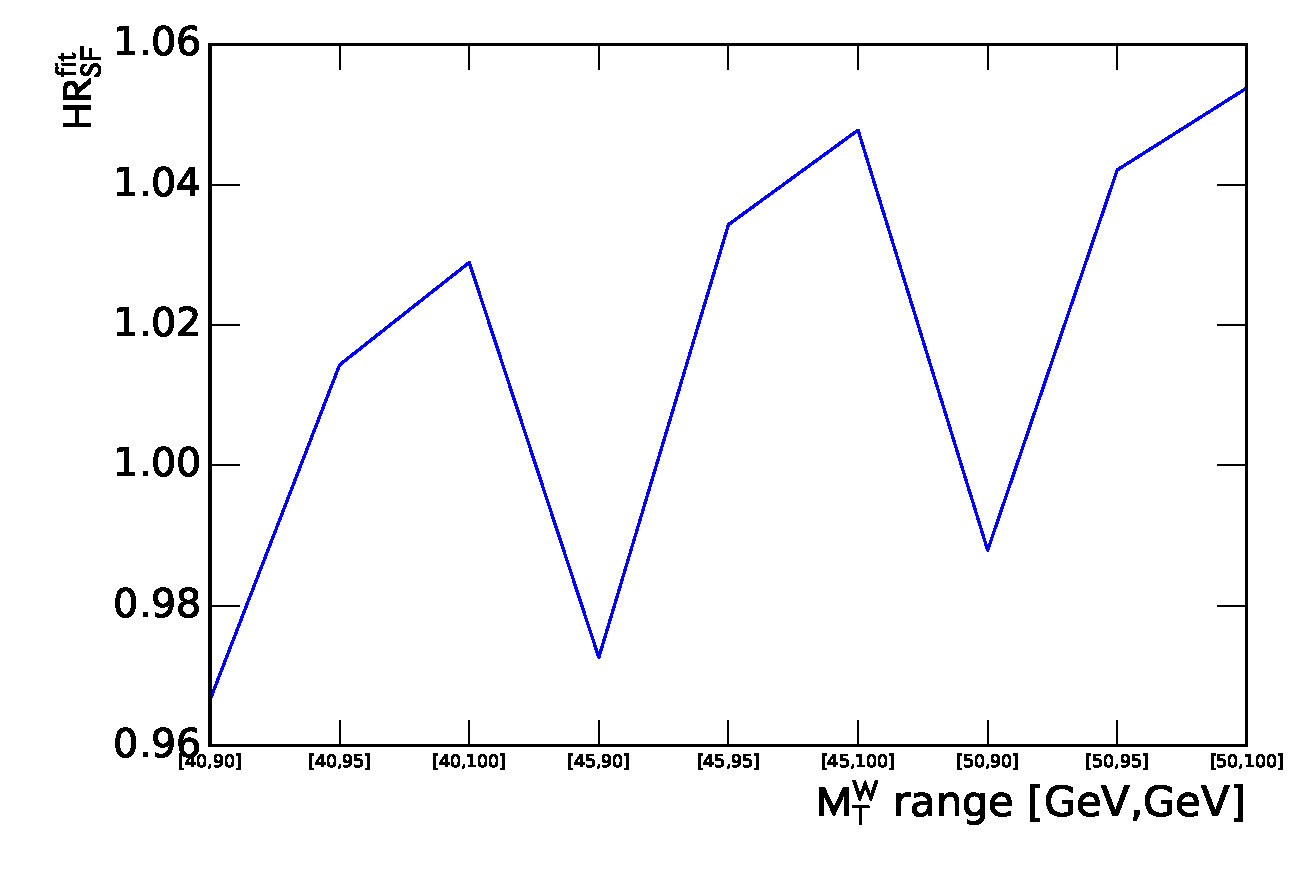
\includegraphics[width=0.7\textwidth]{HadronRecoil/RangeEffect.pdf}
\caption{Values of best hadron recoil biases obtained from the fit for events from combined $W \to l \nu$ selection as a function of fit range. The expected contributions from signals and backgrounds are estimated with Monte Carlo simulation, except for a QCD background, that is not included.}
\label{ScaleMtWRange}
\end{figure}

Distribution of \chiD for different W selections is shown in a Fig. \ref{mtWChi2} a). Because of the possible mismodelling of the tail \mtw distribution events with \mtw > 100 GeV are not included in a \chiD calculation. There is a visible peak in the \chiD distribution for events from \wenu selection, coming from the missing QCD background. Hadronic recoil bias parameters are determined through the fit of \chiD distribution in combined $W\to l\nu$ channel with the function from Eq.~\ref{eq:chiD}. The resulting bias is $HR_{SF}=1.02\pm0.06 (stat)$. 

Additionally, a cut on \mtw lower value may be used to reduce the multijet background contamination. The \mtw range introduces ansource of systematic uncertainty in hadronic recoil scale determination. It is estimated by repeating the fit for the different \mtw lower and upper values, as shown in a Fig.~\ref{ScaleMtWRange}. Fit range systematic error is 0.03, that is resulting in overall result for this method $HR_{SF}=1.02\pm0.07$. 


\subsection{Bias determination using \upar distribution}




\begin{figure}[!tbp]
\minipage{0.32\textwidth}
  \center{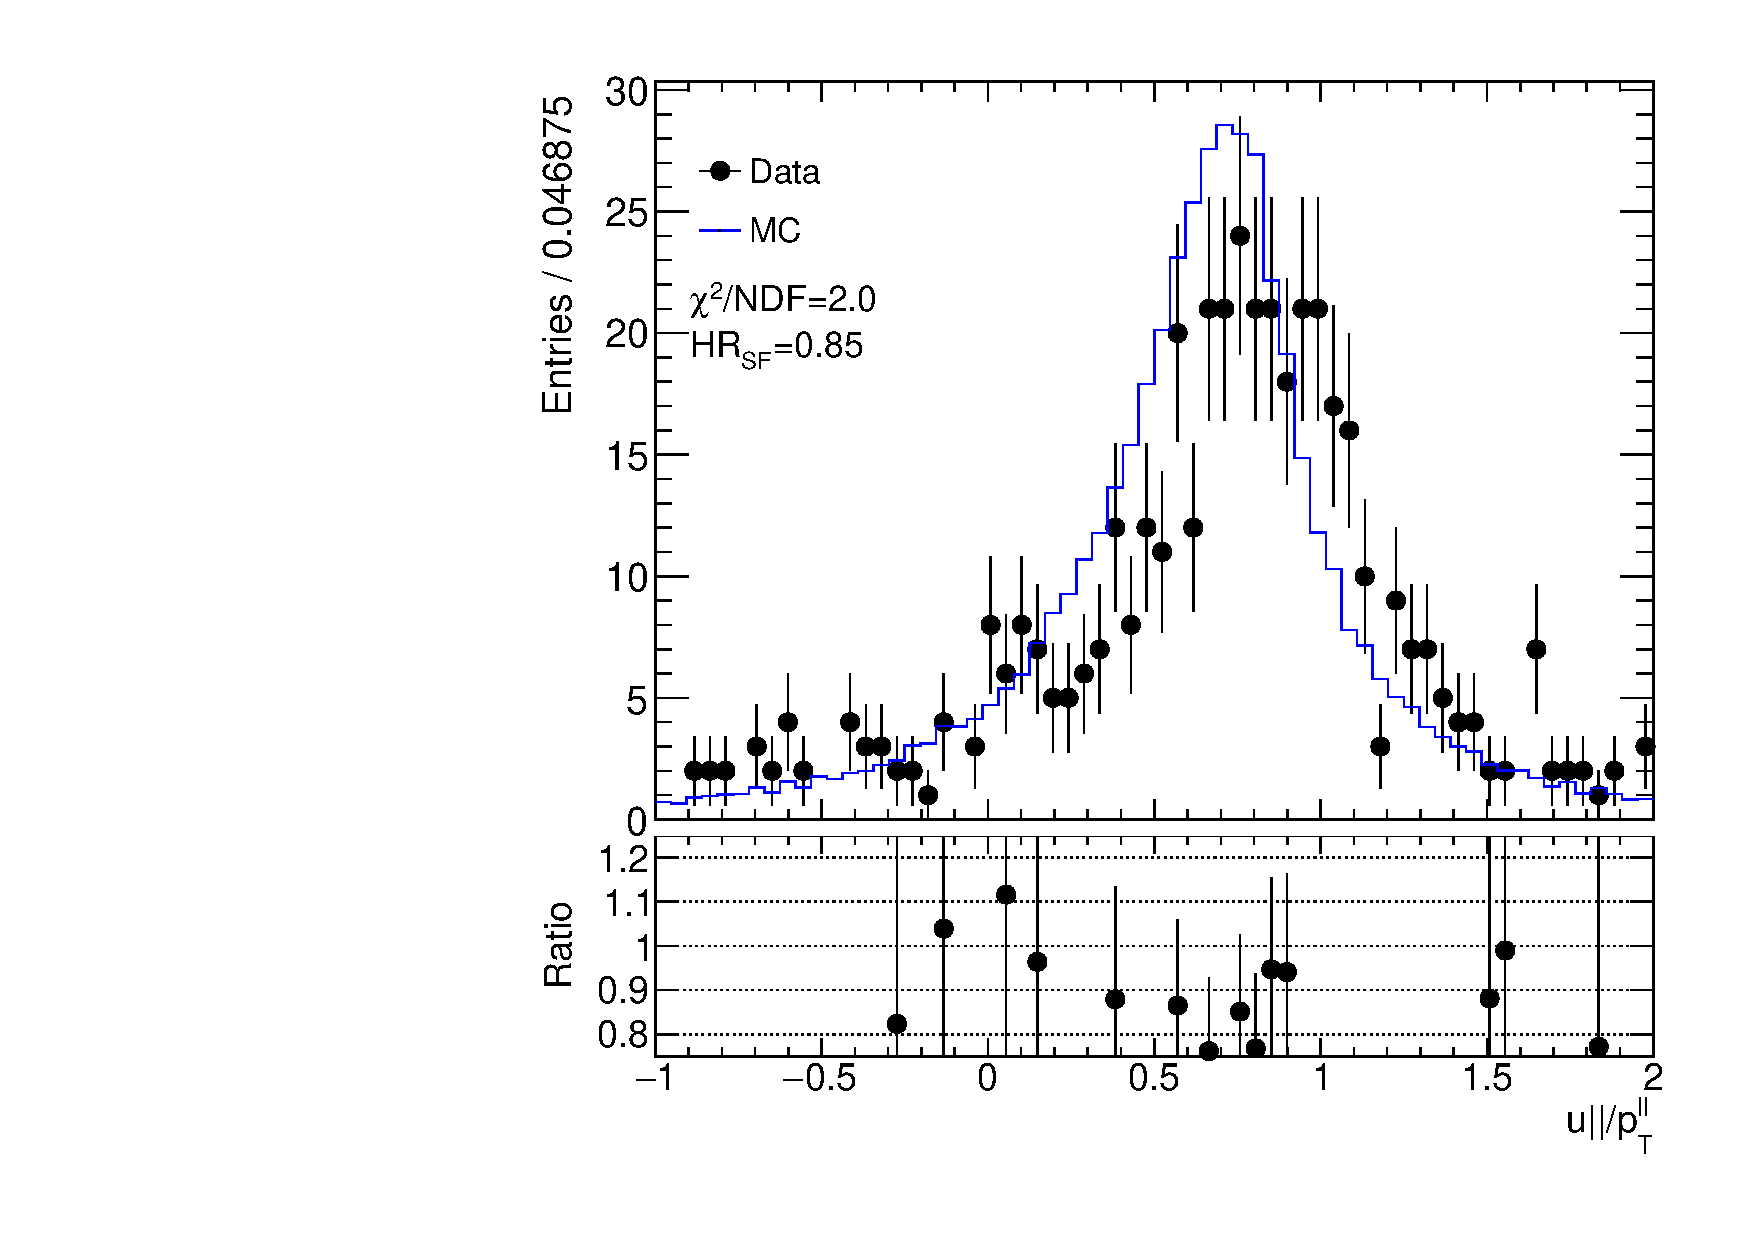
\includegraphics[width=\linewidth]{HadronRecoil/UParEScale5.pdf} a)}
\endminipage\hfill
\minipage{0.32\textwidth}
   \center{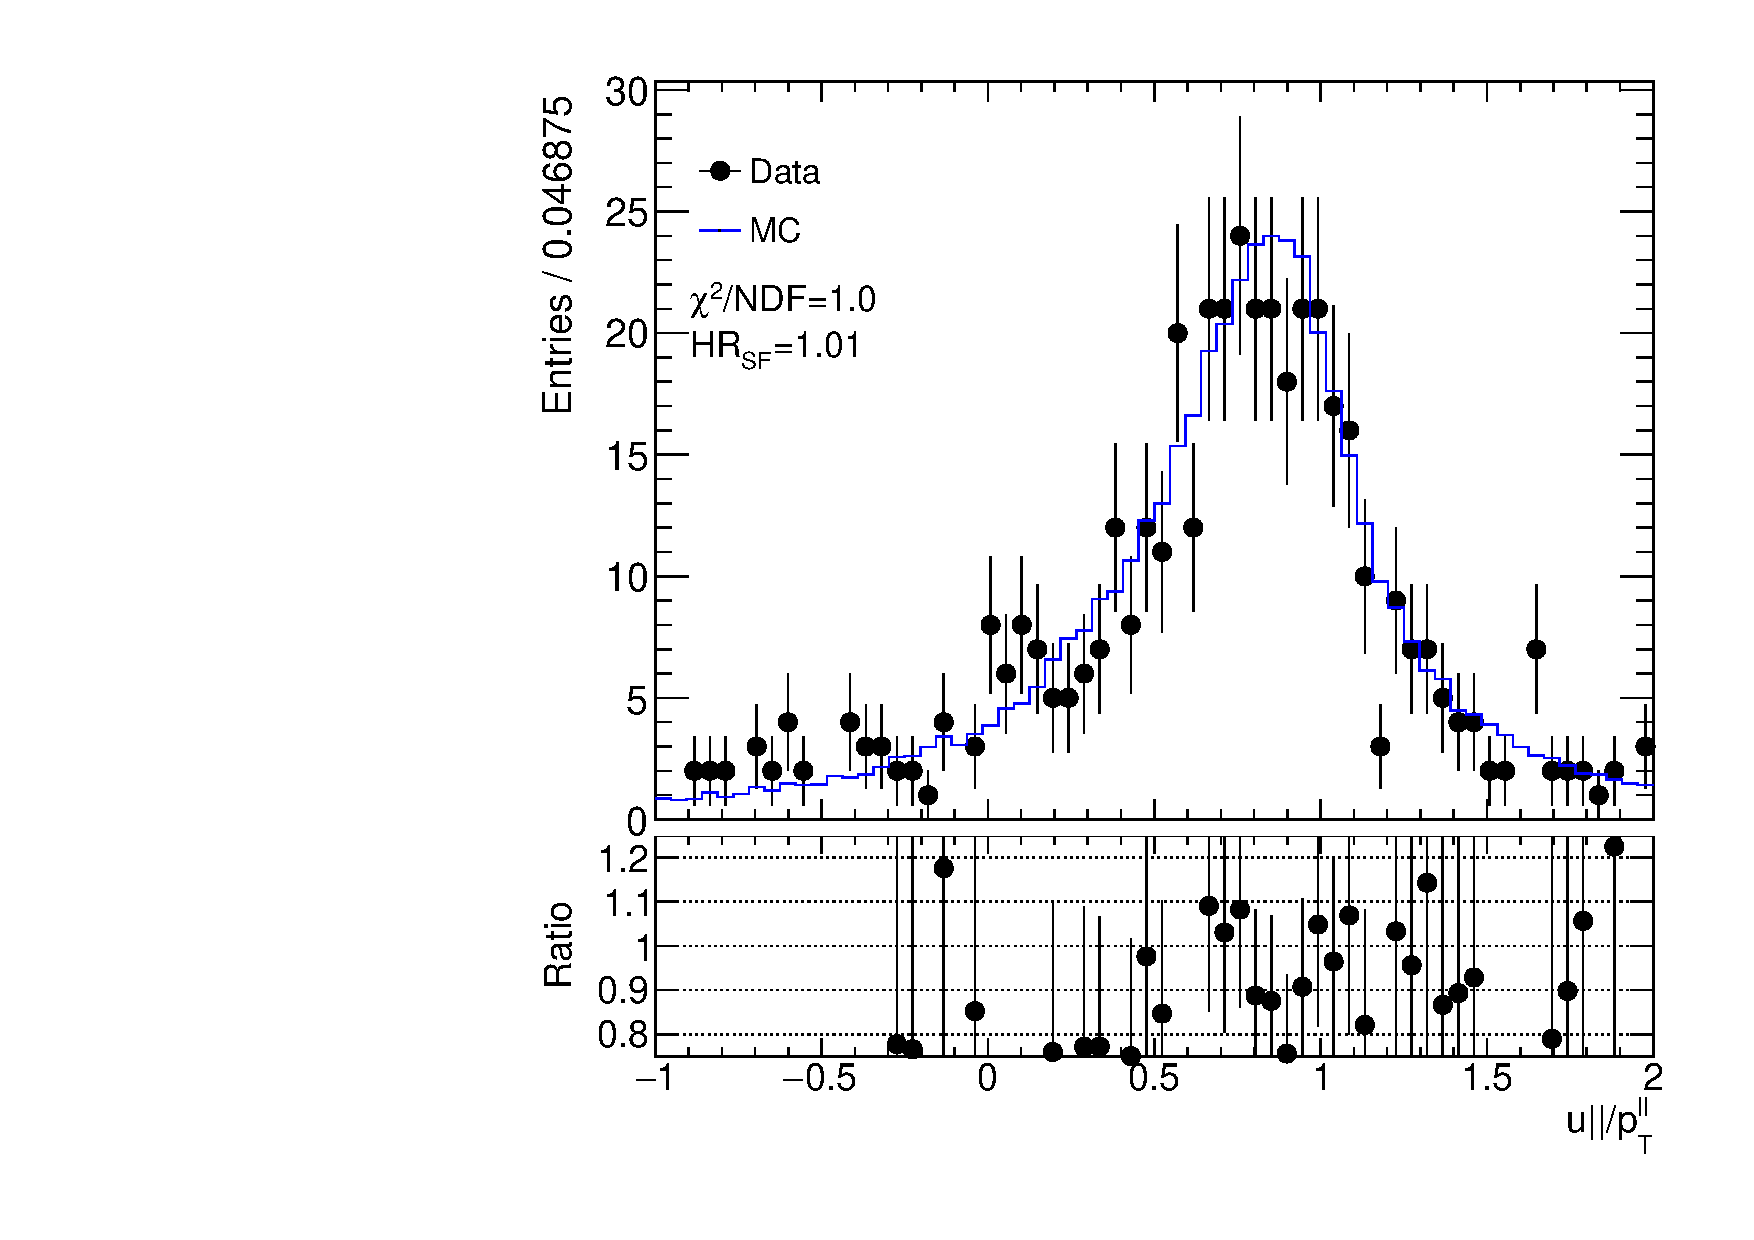
\includegraphics[width=\linewidth]{HadronRecoil/UParEScale13.pdf} b)}
\endminipage\hfill
\minipage{0.32\textwidth}%
   \center{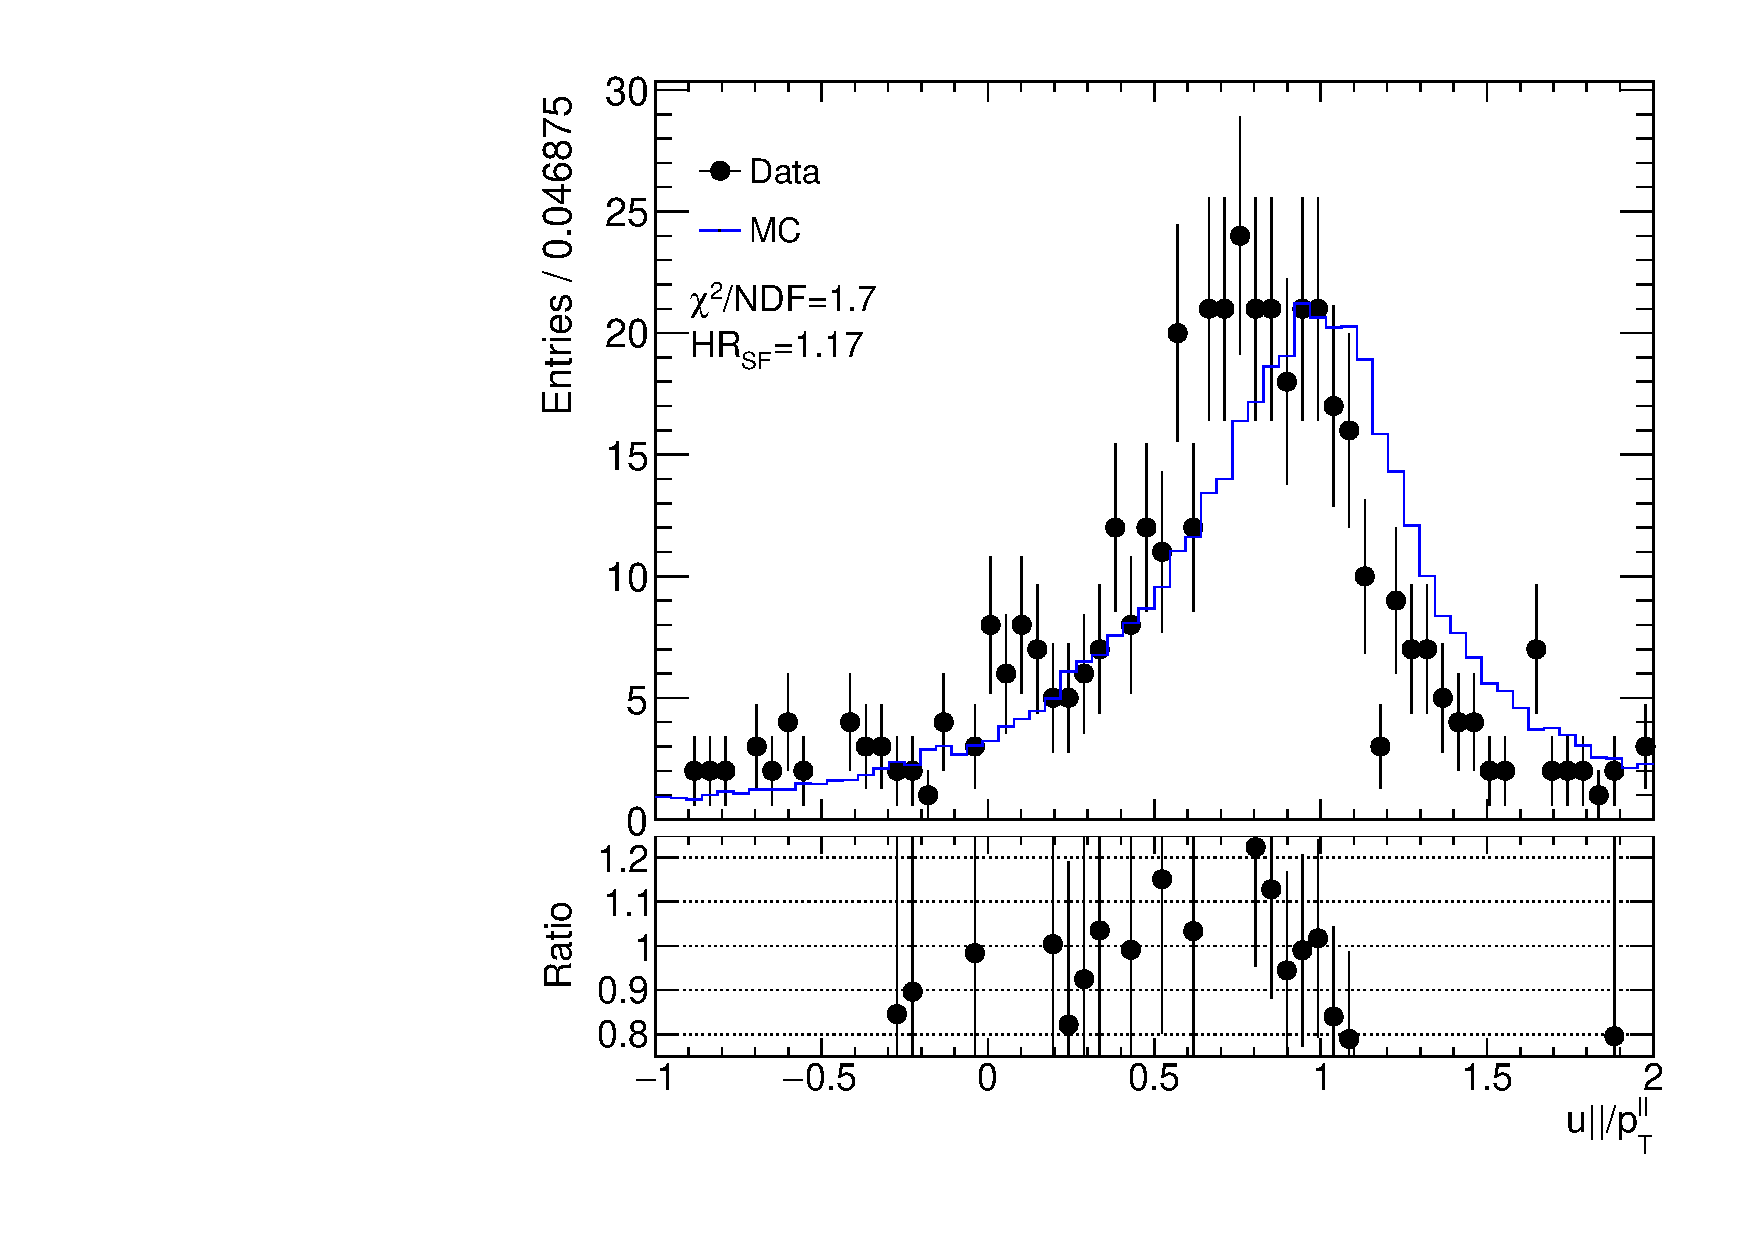
\includegraphics[width=\linewidth]{HadronRecoil/UParEScale21.pdf} c)}
\endminipage
\caption{Parallel hadronic recoil component \upar from the $Z\to ee$ selection for different hadronic recoil scales: a) $HR_{SF}$=0.75 b) $HR_{SF}$= 1.1 c) $HR_{SF}$=1.23. The expected contribution from signal is estimated with Monte Carlo simulation, other background sources are considered negligible.}
\label{HadrRecoil:ZScan}
\end{figure}
 
Similarly to the W channel, scale correction in the Z sample can be determined from the $HR_{SF}$ scan in the $\frac{\upar}{p_T^{ll}}$ distribution, as shown on a Fig. \ref{HadrRecoil:ZScan}. 
Since there is no choise of the range and dependency on $P_T^{bos}$ modeling, there is just one source of uncertainty.


\begin{figure}[!tbp]
\begin{minipage}[h]{0.49\linewidth}
\center{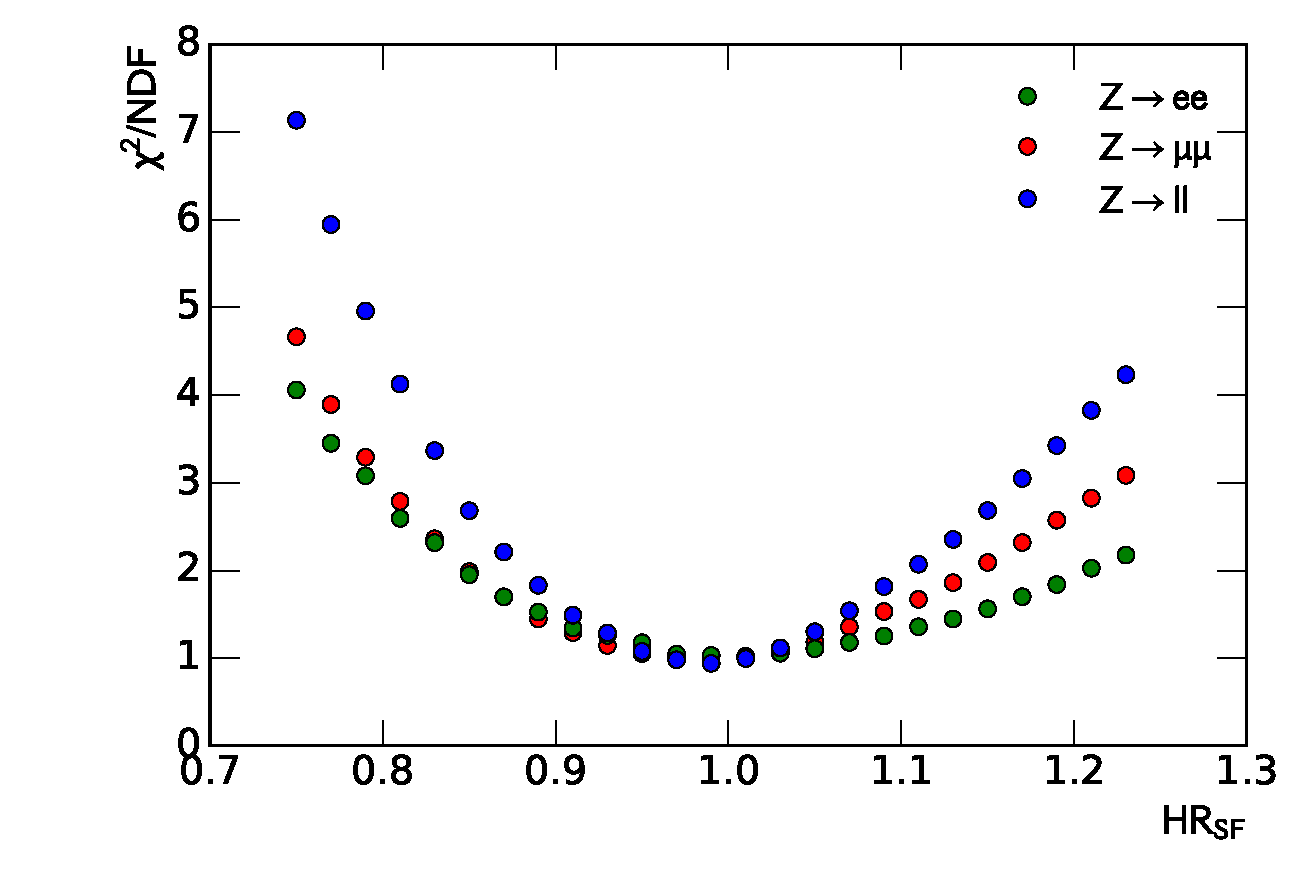
\includegraphics[width=1.\linewidth]{HadronRecoil/chi2Upar.pdf} \\ a)}
\end{minipage}
\hfill
\begin{minipage}[h]{0.49\linewidth}
\center{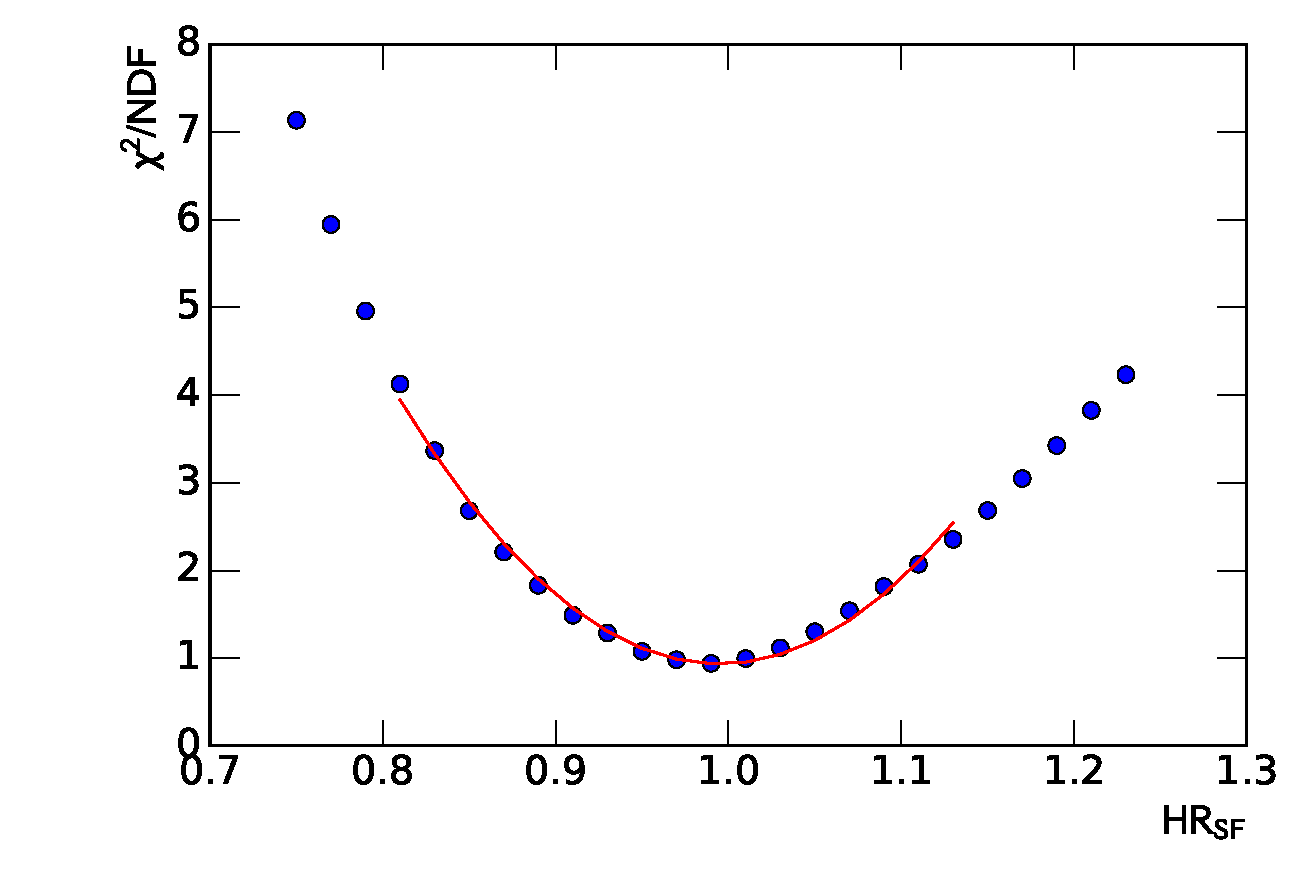
\includegraphics[width=1.\linewidth]{HadronRecoil/chi2UparTot.pdf} \\ b)}
\end{minipage}
\caption{a) Distribution of \chiD  between data and MC for transverse momentum $<\mtw>$ as a function of hadronic recoil scale $HR_{SF}$ for different W boson channels. 
b) Distribution of \chiD  between data and MC for transverse momentum $<\mtw>$ as a function of hadronic recoil scale $HR_{SF}$ for combined $W \to l \nu$ selection. Fit results are shown by a red line.The expected contribution from signal is estimated with Monte Carlo simulation, other background sources are considered negligible.}
\label{uPAr}
\end{figure}  
  
\subsection{Sytematic uncertainty estimation}

Results on a hadron scale factros and it's errors are shown in a Table \ref{tab:SFHadronRecoil}. The results are consistent within 1 sigma. 

\begin{figure}[!tbp]
\begin{minipage}[h]{0.49\linewidth}
\center{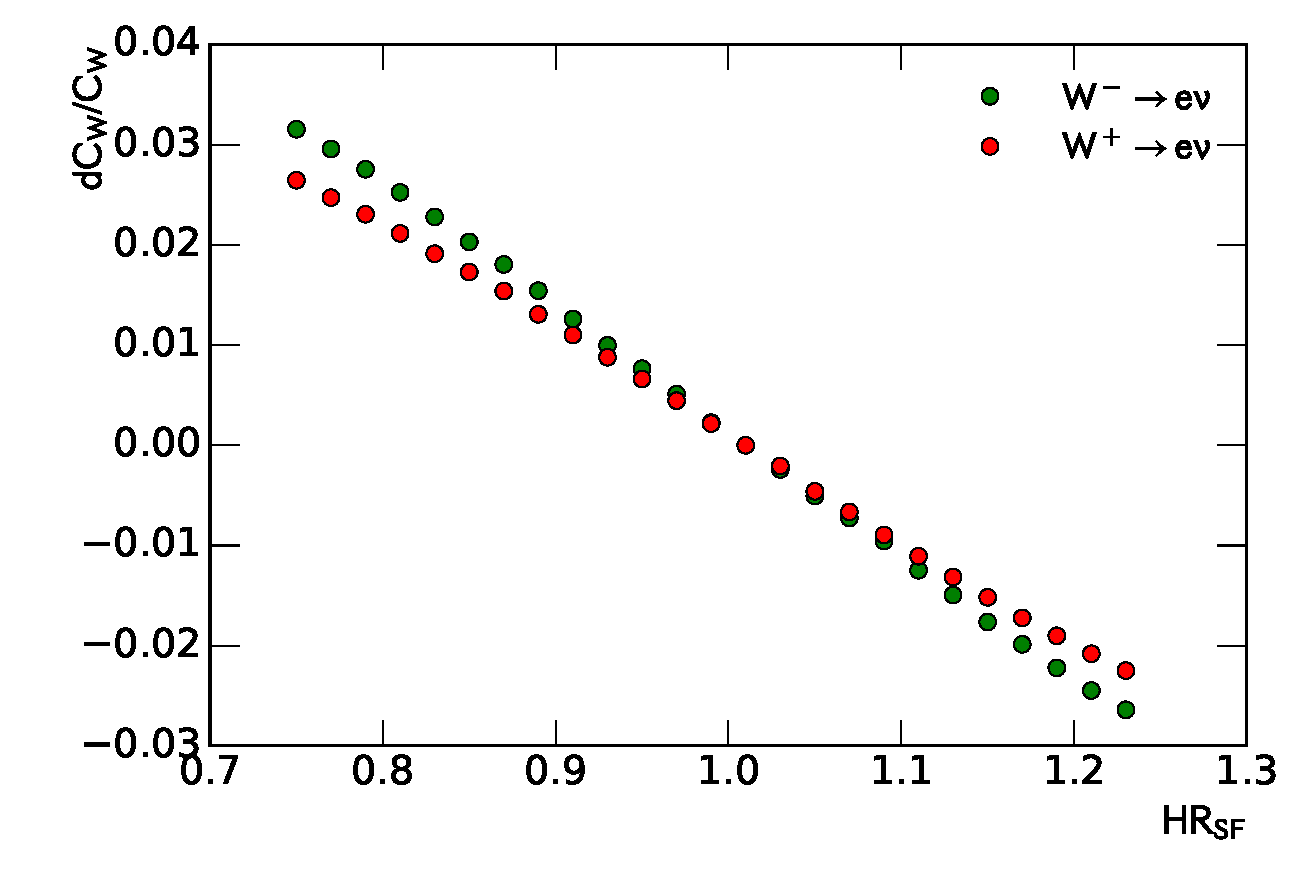
\includegraphics[width=1.\linewidth]{HadronRecoil/CWElectron.pdf} \\ a)}
\end{minipage}
\hfill
\begin{minipage}[h]{0.49\linewidth}
\center{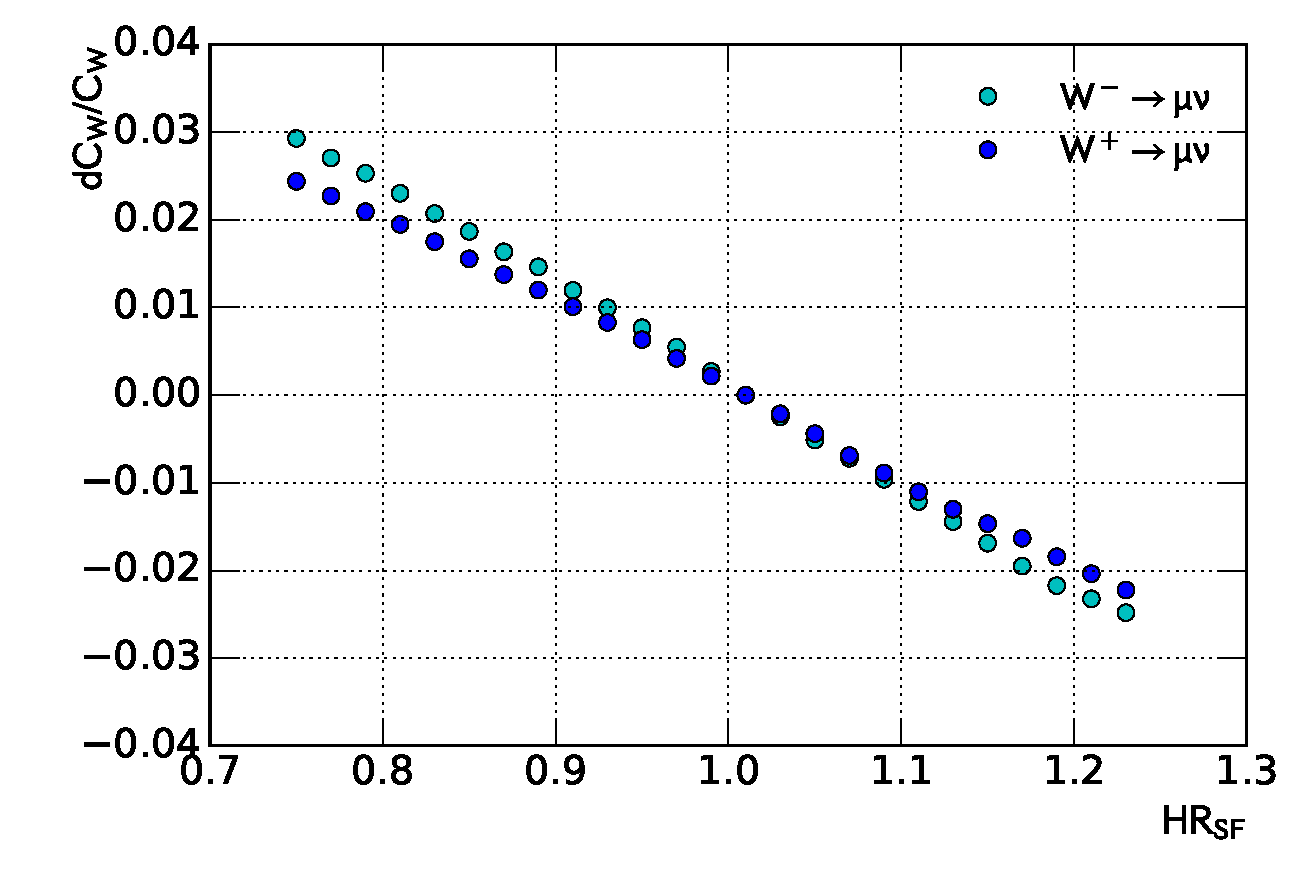
\includegraphics[width=1.\linewidth]{HadronRecoil/CWMuon.pdf} \\ b)}
\end{minipage}
\caption{Effect on a \cw for a different $d\sigma$ for a) \wenu b)\wmunu channel}
\label{ris:Cw}
\end{figure}

\begin{table}[!tbp]
\caption{Hadronic recoil bias determination results and errors for different methods.}
\label{tab:SFHadronRecoil}
\begin{center}
\begin{tabular}{| l | c | c |}
\hline
Method & SF & error \\
\hline
\hline
Mean $M_T^{W}$ & 1.10 & 0.2\\
$M_T^{W}$ \chiD & 1.01 & 0.07 \\
\upar \chiD & 1.00 & 0.014 \\
\hline
\end{tabular}
\end{center}
\end{table}
\section{Summary on hadronic recoil systematics}